\documentclass[12pt]{article}

\usepackage{graphicx}
\usepackage[margin=1in,footskip=0.2in]{geometry}%big footskip brings number down, small footskip brings number up
\usepackage{amsmath}
\usepackage{amssymb}
\usepackage[T1]{fontenc}
\usepackage{listings}
\usepackage{bm}
\usepackage{hyperref}
\usepackage{setspace}
\usepackage[usenames]{color}
\usepackage[utf8]{inputenc}
\usepackage{wrapfig}
\usepackage{relsize}
\usepackage{psfrag}
\usepackage{dsfont}



\hypersetup{colorlinks   = true, %Colors links instead of ugly boxes
            urlcolor     = black, %Color for external hyperlinks
	    citecolor    = blue,
	    linkcolor    = black
}


\renewcommand*\contentsname{Table of Contents}

\newcommand{\E}[1]{
        \mathbb{E}\left[~#1~\right]
}

\def \oner {
	\mathlarger{\mathds{1}}
}

\newcommand{\argmin}{\operatornamewithlimits{argmin}}
\newcommand{\argmax}{\operatornamewithlimits{argmax}}
%\DeclareMathOperator*{\argmax}{arg\,max}


\def \Eix {
	\mathbb{E}\left[~\text{I}(\bm{x})~\right]
}

\def \EIx {
	\mathbb{E}\left[~\text{I}(\underline{\bm{x}})~\right]
}

\def \Ix {
	\text{I}(\underline{\bm{x}})
}

\def \ix {
	\text{I}(\bm{x})
}

\begin{document}

%
%
% \input{coverPage.tex}
\pagenumbering{gobble}
\begin{figure}
\vspace{-4cm}
\hspace{-4cm}
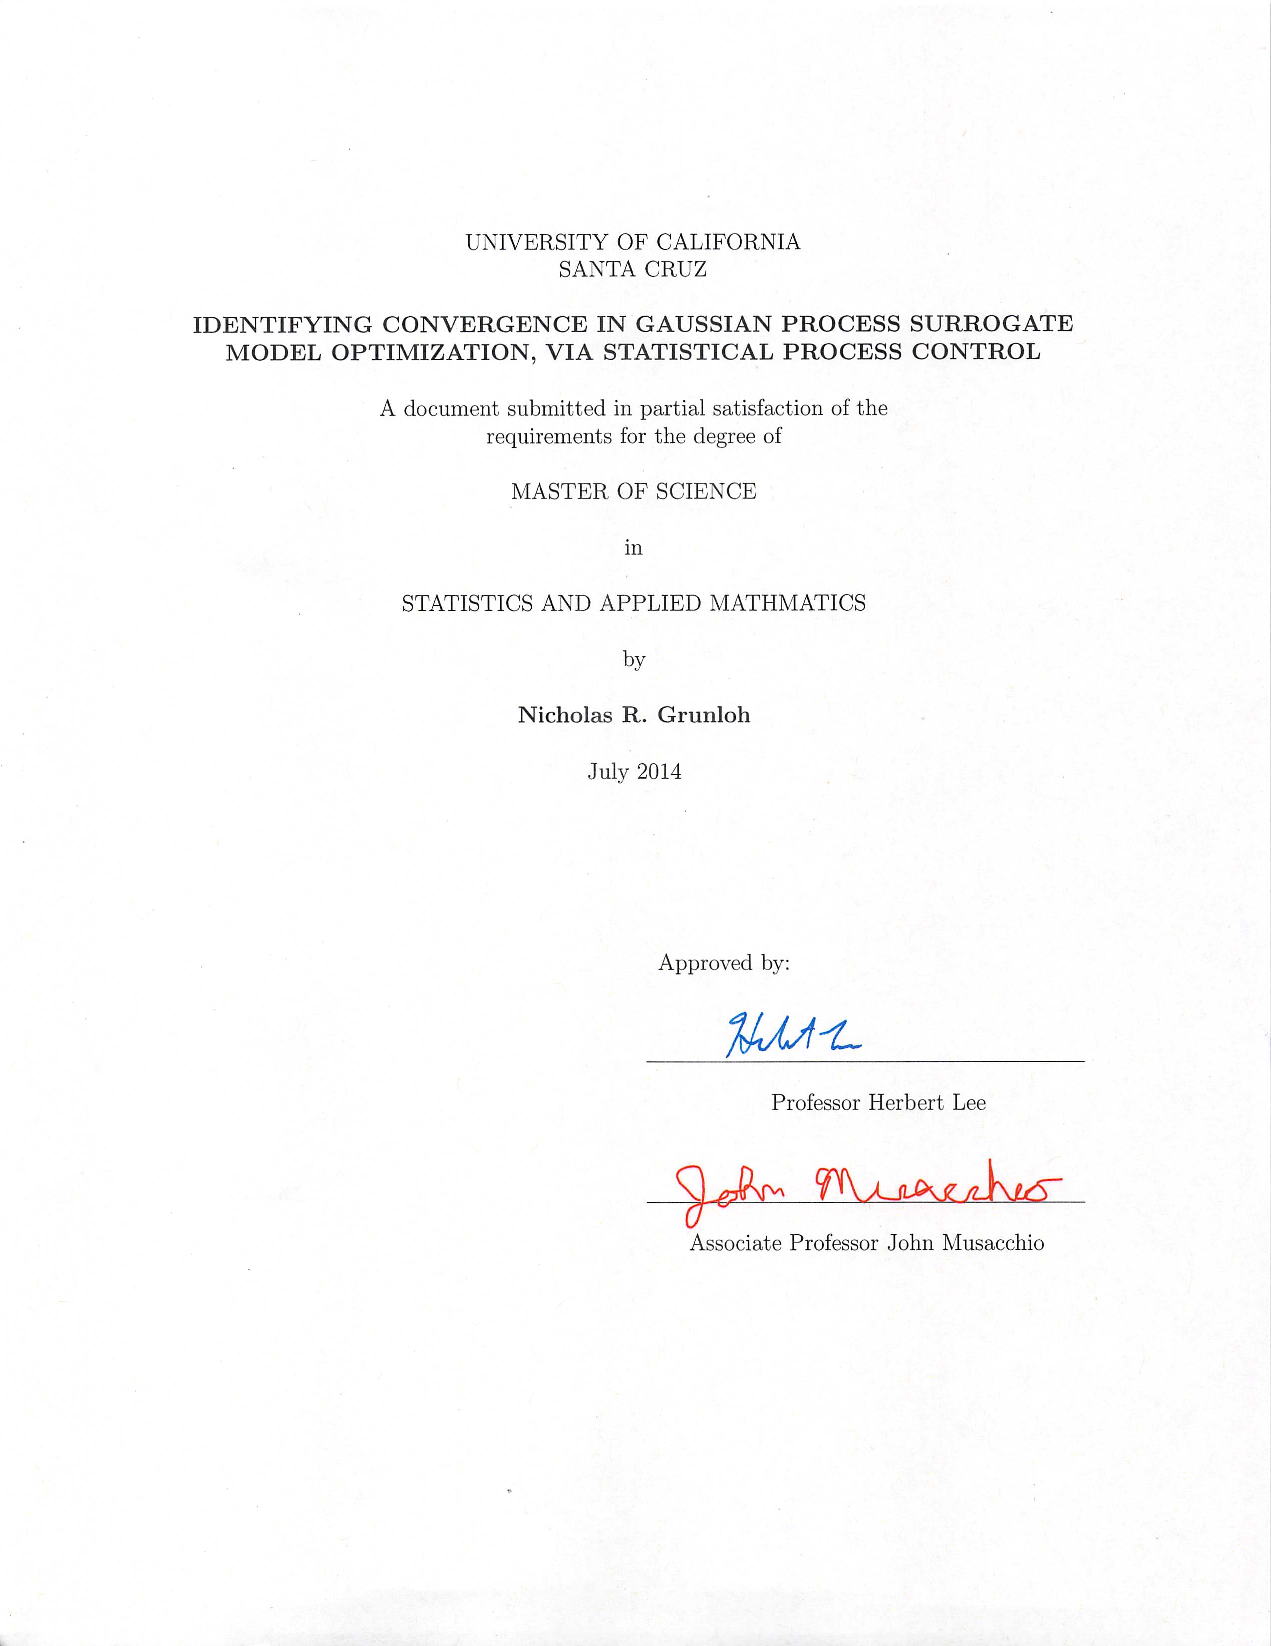
\includegraphics[width=1.5\textwidth]{./figures/titlePage.pdf}
\end{figure}
\clearpage
\tableofcontents
\pagenumbering{roman}
\clearpage
\pagenumbering{arabic}
%
%

\newgeometry{ margin=1in, top=0.70in, footskip=0.4in }
%
%
\begin{abstract}
%due to the subjective nature of convergence 
Identifying convergence in numerical optimization is an ever-present and difficultly subjective task. 
%, sequential design,
The statistical framework provided by Gaussian Process surrogate model optimization provides useful secondary measures for tracking optimization progress; however the identification of convergence via these criteria is often still subjective. % it these measures still subjective. % that can be used to identify convergence. 
%to track the expected improvement criterion to make
Ideas originally introduced in the field of Statistical Process Control (SPC) are thus used to define convergence in an objective way. 
% to remove this subjectivity from the identification of convergence.
The Exponentially Weighted Moving Average (EWMA) chart provides an ideal starting point for adaptation to track convergence via the EWMA convergence chart introduced here.
%the construction of a 


%here

%to follow the progress of optimization via  an adapted version of an Exponentially Weighted Moving Average control chart subjectivity can be removed from the decision of weather or not  

% methods used in statistical process control subjectivity can be removed from the search from convergence. 
%ideas  Through the use of SPC ideas the EWMA convergence chart attempts to give
% convergence a more objective definition.
% \begin{verbatim}
% 
% 
% 
% 
%                      _______________
%                     < Abstract here >
%                      ---------------
%                             \   ^__^
%                              \  (**)\_______
%                                 (__)\       )\/\
%                                  U  ||----w |
%                                     ||     ||
%                 
%                 
%                 
%                 
% \end{verbatim}
\end{abstract}
\doublespacing
%
%


%
\section{Introduction}
	%{\color{red}loaded}
	Convergence is a bit of a loaded word, that is used in many different quantitative contexts.
	%
	In many cases the notion of ``convergence'' can be a frustratingly soft idea, often with an oddly subjective definition and fuzzy interpretation.  
	%
	In each different context of the word, ``convergence'' may have a slightly different meaning, and with it, ``convergence'' may carry different implications about the problem at hand.
	%typical definition implications
	Within the setting of optimization, convergence usually just indicates that we can stop iterating our routines, but even within optimization, convergence can look drastically different from routine to routine.
	%
	In this paper I aim to give ``convergence'' a more concrete definition in the context of Gaussian process surrogate model optimization.
	
	%
	%
	
	% an equally stochastic nature. in this context is thus  stochastic in nature thus
	By the nature of the stochastic exploration procedures inherent to Gaussian process surrogate model optimization, convergence is also stochastic in nature. 
	%
	Unlike other methods, such as gradient descent or pattern search, convergence in Gaussian process surrogate model optimization is not as straightforward as monitoring a vanishing step-size.
	%
	In Gaussian process surrogate model optimization the step-size, between locations of function evaluations, is a largely varied random variable and thus it is not a particularly telling feature of the progress of the objective search.
	%
	Among many practical surrogate modeling applications the claim of convergence may simply depend on the available computation time and the adequacy of the current best solution.
	%Rather,
	However it is obviously preferred to have metrics which expressly indicate convergence.
	%have often been used in a case-by-case manner to ad hocly diagnose convergence .
	For this purpose, various secondary criteria \cite{gramacy2014}, derived from the surrogate model itself, have been monitored.
	%
	In particular it is common to monitor the maximum expected-improvement (EI) until it simply falls below a specified threshold \cite{windExample}.
	%
	This over simplifies the dynamics of convergence in this setting, as quite small EI values should be expected with some regularity based on the particular topology of the problem and the stochasticity of the criterion itself. 
	%
	For the purpose of formalizing a robust process for tracking this stochastic criterion, I turn to the charting methods of the statistical process control literature.
	%%an alize a concrete definition of convergence in this context.% give convergence a more objectively tangible definition.
	Here I borrow ideas from Shewhart's \cite{shewhartBook} classic notion of control, to chart the EI, and thus form a more accurate and objectively tangible definition of convergence.  

	%
	%
	
	%the topics of optimization and Statistical Process Control (SPC),
	My argument is structured in the following way: Section 1.1 gives a brief overview of context for the optimization used here, Section 1.2 covers the basics of Gaussian process surrogate models, and Section 1.3 explains how these models have been used as efficient derivative-free optimization routines.
	%In Section 1.4 I introduce the use of $\EIx$ as a convergence criteria, and in Section 1.5 I provide a more in-depth discussion of the specific SPC charts needed to track this metric so as to consistently identify convergence.
	%$\EIx$$\EIx$ (EI)expected-improvement
	In Section 1.4 I introduce the use of EI as a convergence criterion, and in Section 1.5 I provide a more in-depth discussion of the statistical process control (SPC) logic I use to consistently identify convergence, via the EI criterion.
	%I use for
	In Section 2 I tie all of these topics together to outline a charting procedure to identify convergence in a robust way.
	% on several classic optimization test functions as well as {\color{red}on the Lockwood data}.
	Finally, in Section 3 I provide some examples of identifying convergence via the methods outlined in Section 2. 
	
	%
	%
	\subsection{Overview}
	%\subsubsection{Optimization Overview}
	%\subsubsection{Optimization}
	%
	%
	
	%enormous best choice?{\color{red}enormously}
	Derivative-free optimization is an enormously practical and commensurately difficult task.
	%gradient descent is very eager, perhaps too eager to find optima
	Derivative information has the capacity to efficiently, and rather intuitively, lead the user to an optimal solution. %, as well as, the capability to signal that such an optimum has been found.
	%
	However, derivative information tends to be focused locally, around the starting location of the objective function search, and thus can easily get stuck at local optima.
	%
	Furthermore, derivative information is often not available in many practical problems.
	%
	%we are left quite literally no knowing which way is up :)
	When derivatives are not available we are left to find more creative ways of figuring out which way is up.
	%
	Examples of this creativity can be seen in the diversity of different techniques employed by some of the more popular methods for derivative-free optimization.
	
	%
	%
	
	%evolutionary/genetic; surrogate model
	Examples of effective, and greatly varying, derivative-free optimization strategies include: evolutionary algorithms (EA), simulated annealing (SA), pattern search (PS), trust region methods, as well as surrogate model approaches. 
	%
	Although widely varied, fundamentally these methods share three basic components \cite{noGradBook}.
	%new candidate points for evaluation of potentially optimal points.
	Firstly, there is some procedure for exploring the objective function space. 
	%
	Secondly, these methods use derivative-free information from exploratory function evaluations to update the exploratory procedure, and thus, explore more effectively.
	%
	Thirdly, a well rounded optimization routine is tasked with accurately identifying when it has found an optimal point.
	%
	By tweaking any one of these components, an optimization routine's behavior, with respect to scope, convergence, and accuracy, may differ dramatically.
	%
	Thus, an ideal optimization routine would explore a large space quickly, and it would tell you that it has converged to an accurate solution with minimal information required from the objective function.
	% optimization
	Of course, an optimization routine which embodies {\it all} of these characteristics does not exist, as of yet, but these are good characteristics to consider when choosing the best optimization routine for a particular problem.

	%
	%

	%of derivative-free optimization and identify convergence of
	In particular, I consider the convergence properties of Gaussian process surrogate model approaches.
	%
	The basic idea of surrogate model approaches is to create a statistical approximation (i.e. a model) of the objective function, and use this model to effectively search the objective landscape. 
	%
	Surrogate model-based approaches are primarily of interest due to their ability to deal with functions that are computationally expensive to evaluate because they take special care to minimize the number of objective function evaluations.
	%
	%The typical approach is to minimize the number of function evaluations needed, by using each function evaluation as data to construct a Gaussian process model of the objective function .
	The typical choice of model in the construction of a surrogate model-based optimization routine is a Gaussian process model \cite{gpSurrogate}.
% 	%
% 	Gaussian 
% 	The philosophy in the choosing a Gaussian process model comes from the parral spacial statistics 
	%
	The idea is to work out the next best point to explore by using the surrogate model instead of the objective function.
	%
	Working with the surrogate model saves objective function computation time, and further more, allows for a careful statistical search of the objective function. 
	%in Gaussian process surrogate model approaches; % surrogate model optimization schemes.
	I demonstrate how further analysis of Gaussian process surrogate models can be used to identify convergence in this setting.  

	%
	%
	\subsection{Gaussian Process Models}
	%
	%
	
	%
	Gaussian Process (GP) models often arise naturally in the context of spatial statistics. 
	%their use b
	In fact, GP models often go by the name kriging due to Danie G. Krige who pioneered the use of GPs in the context of Geo-spatial data related to mining \cite{kriging}.
	%  subject of GP models (i.e. $f$)%it can often be instructive to visualize the process spatial
	Thus, it can often be instructive to think about the objective function, $f$, in the context of a spatial application rather than as an abstract mathematical function, since often times $f$ can resemble, or even actually represent, the classical spatial problems. 
	%and stationary% rethe mapping provided by $f$ is a reasonably smooth and stationary process for relating points in the domain, $\bm{x}$. %, by their relative distances from each other.
	The choice of a GP as a surrogate model for $f$ hinges on the fundamental idea that $f$ provides a reasonably smooth mapping for relating points in the domain, \textbf{x}, to response values, $z$(\textbf{x}). 
	%spatial reference?
	That is to say, if we have any hope of finding optima of $f$, we impose the idea that points close together in the domain should have values in the response that are predictably, and similarly, close.
	%might expect if $f$ represent  similarly based  characteristics $f$ were to represent a bringing these inferential biases into the model of
	Regardless of the true interpretation of $f$, by modeling $f$ in this way we may expect $f$ to behave, at least in part, as a spatial quantity; for instance $f$ may just as well represent the elevation of a mountain in space. 
	%
	
	%
	%
	
	% from a particular GP
	A formal statistical perspective expresses a GP as an infinitely dimensional generalization of the multivariate normal distribution, such that every realization of a GP is a normal random variable and jointly all such realizations form a multivariate normal distribution. 
	%
	Typically the mean response is modeled using a linear combination of simple basis functions, $\bm{\beta}^\intercal \text{\textbf{f(x)}}$, with a zero mean random process error term, $\epsilon$(\textbf{x}), such as,
	%
	\begin{equation}
	z(\bm{x}) = \bm{\beta}^\intercal \text{\textbf{f}}(\bm{x}) + \epsilon(\bm{x}) + \eta(\bm{x}).
	\label{baseEq}
	\end{equation} 
	%Here the $\bm{\beta}$ are trend parameters and  
	Here $\eta(\bm{x})$ is Gaussian noise, and $\epsilon(\bm{x})$ is fundamentally governed by a correlation function, $ K(\bm{x}, \bm{x}')$, such that the covariance is $C(\bm{x}, \bm{x}')=\sigma^2K(\bm{x}, \bm{x}')$. 
	%the distance between \textbf{x} and \textbf{x}$'$
	By specifying a homogeneous correlation function, we thus model the relationship of $||\bm{x}-\bm{x}'||$ with the correlation structure that we expect to see when jointly considering two such realizations of the GP.
	%For example, tone such 
	The following exponential power family provides a common example of such a choice of $K(\bm{x}, \bm{x}')$,
	%
	\begin{equation}
	K(\bm{x}, \bm{x}') = \exp\left\{ -\frac{||\bm{x}-\bm{x}'||^p}{d} \right\}.
	\label{corrFunc}
	\end{equation}
	%
	Considering Eq. (\ref{corrFunc}) for every combination of \textbf{x} and \textbf{x}$'$ among a particular data set provides a correlation matrix \textbf{K}; thus multiplying by $\sigma^2$ creates the likelihood covariance matrix \textbf{C}.
	%
	For further discussion of choices of $K(\bm{x}, \bm{x}')$ see \cite{steinBook}.
	%% Thus we can express this model in  equations (\ref{baseEq}) and (\ref{covFunc}) together as a proper Bayesian model we get,
	Equations (\ref{baseEq}) and (\ref{corrFunc}) imply the following simple Bayesian model, which forms the basis for many other complex GP models  
	%
	\begin{equation}
	\begin{aligned}
	\text{\textbf{Z}} ~|~ \bm{\beta}, \sigma^2, \text{\textbf{K}} &~\sim~ N_n\Big(\text{\textbf{F}}\bm{\beta},~ \sigma^2\text{\textbf{K}}\Big)
	&~ \sigma^2 ~|~ a, b &~\sim~ IG(a, ~b)
	\\
	\bm{\beta} ~|~ \bm{\beta}_0, \text{\textbf{V}} &~\sim~ N_m\big(\bm{\beta}_0,~ \text{\textbf{V}}\big) &~
	\text{\textbf{V}} ~|~ \bm{\Psi}, \nu &~\sim~ IW\big(\bm{\Psi}, ~\nu\big).
	\label{gpModel}
	\end{aligned}
	\end{equation}
% 	%
	Here $a$, $b$, $\bm{\beta}_0$, $\bm{\Psi}$, and $\nu$ are fixed hyper-parameters of the model, and $N$, $IG$, and $IW$ represent the Multivariate Normal, Inverse-Gamma, and Inverse-Wishart distributions respectively.
	%
	Model (\ref{gpModel}) specifies a mostly conjugate, Gibbs sampling, inference setting with the exception of the covariance structure parameters, which require Metropolis-Hastings sampling \cite{gpJasa}.
	
	%
	%
	
	%
	Bayesian models of this type, not only provide effective inference on $f$, but they provide a framework for prediction that allows for further efficient exploration of $f$.
	%
	In the Bayesian perspective, the parameters of Model (\ref{gpModel}) are random variables.
	% of these parameters over the parameters. allow a in the data
	Thus doing inference on these parameters, via MCMC, results not only in point estimates, but entire distributions that completely, and flexibly, describe the present uncertainty. 
	%
	%It is thus desirable to compute accurate empirical intervals based on these samples, rather than rely on the classical asymptotic theory.
	%
	%As to be discussed in section 2, the assumptions of the classical asymptotic theory may be hard to satisfy, and thus credible intervals are preferred here. 
	%sample based used to do inference on models like Model (\ref{gpModel})
	%that not only allows for
	Furthermore Bayesian methods, such as Model (\ref{gpModel}), provide a complete predictive framework for estimating function behavior in unobserved candidate locations, as well as full distributional uncertainty characterization of these unseen locations.
	%can be used to construct the posterior predictive distribution for new candidate locations of $f$.
	%several of which candidate locations may provide good potential of these 
	By considering the uncertainty and expected behavior of the posterior predictive GP surface across candidate locations, it is thus possible to make informed decisions about where to search for new optima \cite{taddyOpt}.
	
	%
	%
	
	%
	In many cases the assumption of a smooth $f$ with a homogeneous uncertainty structure can provide an effective and parsimonious model.
	%
	However for the sake of providing a flexible surrogate model, it is desirable to have the ability to loosen these restrictions in cases when $f$ looks more like the Grand Canyon, as opposed to the Great Plains.     
	%objective landscape
	Gramacy and Lee \cite{gpJasa} introduce the idea of allowing this flexibility via a treed partitioning of the domain.
	%
	This allows separately stationary GP surfaces to fit separately stationary portions of $f$.
	%
	For further explanation of partitioned Gaussian process models as well as notes on implementing such models in R, see the R package \verb tgp  \cite{tgp}.
	
% 	\newgeometry{ margin=1in, footskip=0.4in }
% 	\doublespacing
	%
	%
	\subsection{Optimization}
	%
	%
	
	%
	In explaining the construction of optimization routines based on statistical models like model (\ref{gpModel}) as described by \cite{taddyOpt}, I view the typical surrogate optimization procedure in terms of the three basic components of optimization that I outline in Section 1.1.1. 
	%
	Firstly, I identify the type of information that has been used in Gaussian process models to effectively explore $f$.
	%
	Secondly, I outline the exploration procedure, and how a Gaussian process updates its exploration of $f$ using this information.
	%\\\\
	For the sake of making a concrete argument, I focus
	on optimization in the context of minimization, but all of these ideas can easily be applied to finding maxima by simply minimizing $-f$.

% 	\restoregeometry
% 	\doublespacing
	%
	%
	\subsubsection{Expected Improvement}
	%
	%

	%$\Eix$ \cite{eiOpt},
	In finding minima via Gaussian process models, the expected-improvement (EI) criterion has been used \cite{tgp2}, \cite{taddyOpt} to identify candidate points that have the strongest {\it possibility of encountering new minima}.
	%when applied to a single candidate point has
	The EI criterion is fundamentally based on the improvement criterion for each candidate location of the following form,
	\begin{equation}
	\ix~=~ \max \Big\{ \big(f_{min} - f(\bm{x})\big), ~0 \Big\}
	\label{ix}
	\end{equation}
	%
	In expectation, the $\Eix$ criterion rewards candidate points not only for a low predictive mean, but also rewards the high uncertainty associated with poorly explored regions.
	%
	Considering Bayesian models like Model (\ref{gpModel}), we can most efficiently use information in our model by considering $\Eix$ with respect to the posterior predictive distribution.
	
	%
	%
	
	%
	%{\color{red}
	By the nature of the Bayesian construction of models like Model (\ref{gpModel}), criteria such as the improvement criterion, $\ix$, are random variables, and as such, we can learn their distributions via Markov Chain Monte Carlo (MCMC) methods.
	% each candidate location has a $\ix$ is a random variable, at each candidate location, who's distribution is easily accessible via the MCMC sample-based implementation of the model, as described in \cite{tgp}.
	%}Thus f; predictive For each candidate location t%, and using these samples to derive the .
	The distribution of $\ix$, a posteriori, can be obtained by considering samples from the posterior predictive distribution at each candidate location and computing the necessary statistics to form $\max \Big\{ \big(f_{min} - z(\tilde{\bm{x}})\big), ~0 \Big\}$ as an approximation of Eq. (\ref{ix}).  
	%\EIX is not quite right it should just be the single location formula
	Furthermore, the mean of these posterior predictive $\ix$ samples provide an empirical solution for finding an EI for each candidate location \cite{tgp2}.
	%same issue here EI criteria described in Eq. (\ref{EIx}), with $g=1$.
	Thus, truncating these $\ix$ samples at 0 and finding the candidate location with the maximum $\Eix$, identifies the EI criterion described.

% 	\clearpage
        %
        %
        \subsubsection{Exploration Procedure}
        %
        %
        
	%
	%
	\begin{wrapfigure}{r}{0.5\textwidth}
	\vspace{-1.6cm}
% 	\vspace{-2.5cm}
	\singlespacing
	\caption{Optimization Procedure}
	\begin{itemize}
	\item[1)] Collect an initial set, $\bm{X}$.
	\item[2)] Compute $f(\bm{X})$.
	\item[3)] Fit GP model based on evaluations of $f$.
	\item[4)] Collect a candidate set, $\tilde{\bm{X}}$.
	%\item[5)] Compute $\Eix$ among $\tilde{\bm{X}}$.$\E{\text{I}(\tilde{\bm{x}_i}})$
	\item[5)] Compute EI among $\tilde{\bm{X}}$
	%\item[6)] Add $\tilde{\bm{x}_i}$ yielding largest $\Eix$ to $\bm{X}$.
	\item[6)] Add $\argmax_{\tilde{\bm{x}_i}} \E{\text{I}(\tilde{\bm{x}_i})}$ to $\bm{X}$.
	\item[7)] Check convergence.
	\item[8)] If converged exit. Otherwise go to 2).
	\end{itemize}
	\doublespacing
	%\vspace{-0.85cm}
	\label{procedure}
	\end{wrapfigure}
	%
	%
	
	% us with a
	The idea for optimization, in this context, is to only evaluate the objective function at locations that have a good chance of providing a new minimum. 
	%I need a handle
	An optimization scheme based on models like Model (\ref{gpModel}) starts by initially collecting a set, $\bm{X}$, of locations to evaluate the true function, $f$, to gather a basic impression of $f$.
	% (\ref{gpModel})
	A GP model is then fitted with $f(\bm{X})$ as observations of the true function.
	%EI
	Using this model, a set of candidate points, $\tilde{\bm{X}}$, are randomly selected from the domain and the EI criterion is calculated among these points.
	%
	The candidate point that has the highest EI is then chosen as the best candidate for a new minimum and thus, it is added to $\bm{X}$.
	% (\ref{gpModel})
	The objective function is evaluated at this new location and the GP model is refit based on the updated $f(\bm{X})$.
	%
	The optimization procedure carries on in this way until convergence.

	
	%
	%
	\subsection{A Convergence Criterion}
	%
	%
	
	
	%
	Iterating the above mentioned optimization procedure and tracking the value of EI at each iteration gives the user a sense for what the algorithm thinks is left to learn about finding a minimum of $f$.
	%
	For instance, recall that EI is giving us information about the {\it possibility of encountering a new optimum}.
	%
	For determining convergence, you can imagine exploring $f$ with respect to EI, in the following way.
% 	%
	Initially, as we enter the objective landscape of $f$, we do not really know what to expect.
	%
	However we set-out to explore this space, and as we explore, we develop expectations about the topography of $f$.
	%
	Each exploratory sample of $f$ provides some potential for a new optimum, although as we learn more about this function, the expectation that we will see something new begins to diminish.
	%
	If we continue to explore\\ this landscape, we will come to understand the environment so well that we will virtually never expect to see something new.
	%
	In fact, continued exploration of the space may become boring.
	%that continued search of the objective function would be has become uninte
	Thus the key to efficiently identifying convergence is to quickly realize that the expectation of finding a new, and substantial, optimum is sufficiently low.
	%%would become uninteresting.
	That is to say, convergence occurs, in this context, when the expectation of finding new minima is low enough, so that continued search of the objective function is expected to be unproductive.

% 	\clearpage
	%
	%
	\begin{wrapfigure}{l}{0.5\textwidth}
	\vspace{-1.1cm}
	\begin{center}
	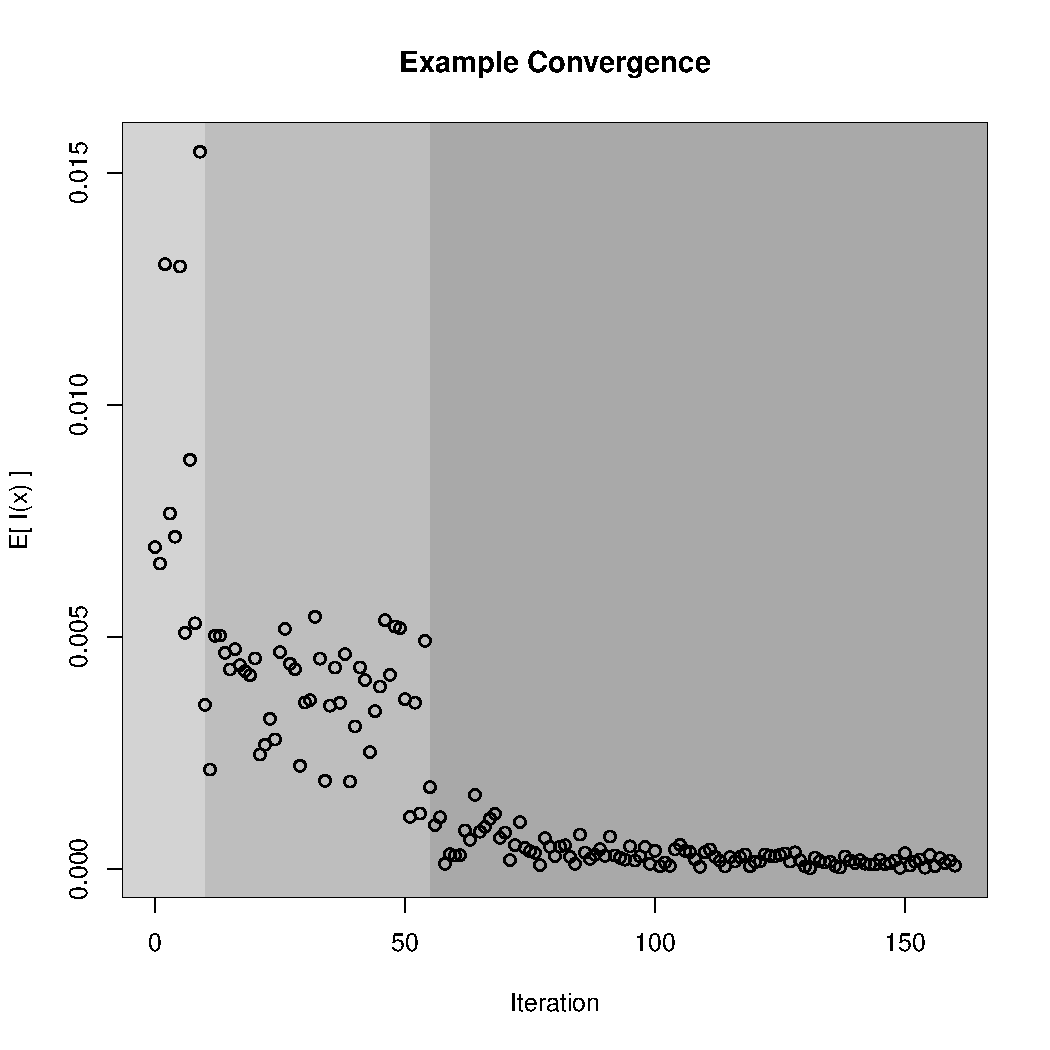
\includegraphics[width=0.5\textwidth]{./figures/exampleEI.pdf}
	\end{center}
	\vspace{-0.85cm}
	\caption{A fabricated EI progression, made to clearly demonstrate the typical three stage convergence pattern.}
	\label{EIxEX}
	\end{wrapfigure}
	%
	%
	
	%stochasticity
	Following from this intuitive story about the behavior of EI; quantitatively EI follows a stochastically non-stationary decreasing function as iterations of the optimization routine pass.
	%
	Initially EI tends to start in at an optimistically high value, depending on the initial size of $\bm{X}$.
	%
	As several iterations of the optimization procedure continue to sweep through, EI tends to enter a fairly stable region of intermediate values where the algorithm is figuring out the major features of $f$.
	%
	Eventually the value of EI will converge in probability to 0, but by construction it can not decrease below 0.
	
	%
	%
	%\subsubsection{Statistical Process Control Overview}
	\subsection{Statistical Process Control}
	%
	%
	
	%{\color{red}the elusively fuzzy concept of} %s sense of the word ``convergence''.
	In identifying convergence, I find the notion of ``control'', from the SPC literature, to be in the same spirit as the notion of ``convergence'' in optimization. 
	%
	In Shewhart's seminal 1931 book \cite{shewhartBook} on the topic of control in manufacturing, Shewhart explains that a phenomenon is said to be in control when, ``through the use of past experience, we can predict, at least within limits, how the phenomenon may be expected to vary in the future.''
	%
	This notion is not only an instructive framework for thinking about convergence, but it offers this framework with a comforting sense of finitude. 
	%
	The phrase ``within limits'' gives us a hope of drawing some line in the sand; turning the previously subjective burden of identifying convergence, into a simple objective task that even a computer can accomplish.
	
	%
	%
	
	%% of that statistic.
	In its most simplified form, SPC  considers an approximation of a statistic's sampling distribution as repeated sampling occurs in time.
	% from some data generating mechanism,
	For example, the $\bar x$-chart tracks the mean of, say $m$, repeated samples, of size $n$, so as to expect the arrival of each subsequent mean in accordance with the typical sampling distribution for the mean, $\bar{x}_j \sim N\left(\mu, \frac{\sigma^2}{n}\right)$.   
	%
	%Shewhart expresses his idea of control as the expected behavior of random observations from the sampling distribution of interest.
	Shewhart expresses his idea of control, in this case, as the expected behavior of random observations from this sampling distribution.
	%
	By considering confidence intervals on this sampling distribution we can easily draw explicit boundaries (i.e. control limits) to identify which samples are in control, and which are not.
	%
	Observations violating our expectations (i.e. observations that fall outside of our confidence interval/beyond the control limits) indicate an out-of-control state.
	%
	Since neither $\mu$ nor $\sigma^2$ are typically known, it is of primary importance to use the data carefully to form accurate approximations of these values, thus establishing a standard for control.
	%
	Furthermore, this logic relies upon the typical asymptotic results of the central limit theorem (CLT), and special care should always be taken to satisfy its requirements.
	
\clearpage
%
%
\section{Identifying Convergence}
%
%
	
	%Considering Figure (\ref{EIxEX}) it is easy to see how tracking EI values could naturally fall into the framework of the SPC logic.
	Figure (\ref{EIxEX}) can bee seen to resemble an $\bar x$-chart, and with some modifications it is not hard see how tracking EI values could naturally fall into the framework of the SPC logic.
	%
	Recall that each point in this figure is the mean of $\ix$ MCMC samples at the most promising candidate location, in the current iteration.
	%as we look back through the previously observed EI values
	Thus as iterations of the optimization procedure pass, we form a repeated sampling situation for the EI values to consider via SPC.
	%presumably converged; new;  control for EI  state of control% is has presumably found convergence.
	The idea behind identifying convergence in this setting, is to establish a state of pre-convergence; we then claim that we have achieved convergence when we observe EI values that indicate a move from this pre-convergence state, into a state of control about some converged EI distribution. 
	
	%
	%
	
	%
	Considering the EI values in this way requires tactful consideration of how to evaluate the arrival of EI observations.
	%
	%Since it is not known when we may stumble across convergence we must be on the lookout for convergence in each iteration 
	%
	In order to achieve the above described perspective of convergence, the goal is to establish control among the most recently observed EI values as they move from the initial pre-convergence values into control.
	%look back through the EI values observed thus far in reverse order.
	Thus, it is necessary to consider the progression of EI values in the reverse order for the sake of SPC. %,  with the most recent observations 
	%
	That is to say, I consider the most recently observed EI value as the first value to be tracked in the SPC repeated sampling.
	%
	This construction allows moving average methods, described in section 2.2, to establish a standard of control that is based on the most up-to-date EI information. 
	%
	In many ways the EI criterion falls naturally into the typical $\bar x$-chart setting, but as we have already seen, careful consideration of the properties of the EI convergence behavior illustrate some practical and theoretical concerns for identifying convergence using the SPC logic.
	
	%{\color{red} I need a more explicate review of $\bar x$ chart, with discussion of control limits.}
	
	%
	Firstly, recall that EI is a stochastically decreasing function of the iteration number. 
	%since there are often few
	The nonstationary decreasing nature of the EI values can easily lead to premature identification of convergence.
	%{\color{red}few}
	The initially very high EI values combined with the overall decreasing trending of the series often sets up a trap which quickly cause initial values to exceed the control limits of an $\bar x$-chart. 
	%
	%Furthermore, the $\bar x$-chart is not made to deal with the overall decreasing nature of the EI values.
	%
	% of the initially optimistic phase while focusing the attention more heavily on recent values of EI.
	%
	I introduce the Exponentially Weighted Moving Average (EWMA) chart as a way of diffusing this effect. 
	
% 	\clearpage
	%
	%
	\begin{wrapfigure}{l}{0.5\textwidth}
	\vspace{-1.1cm}
	\begin{center}
	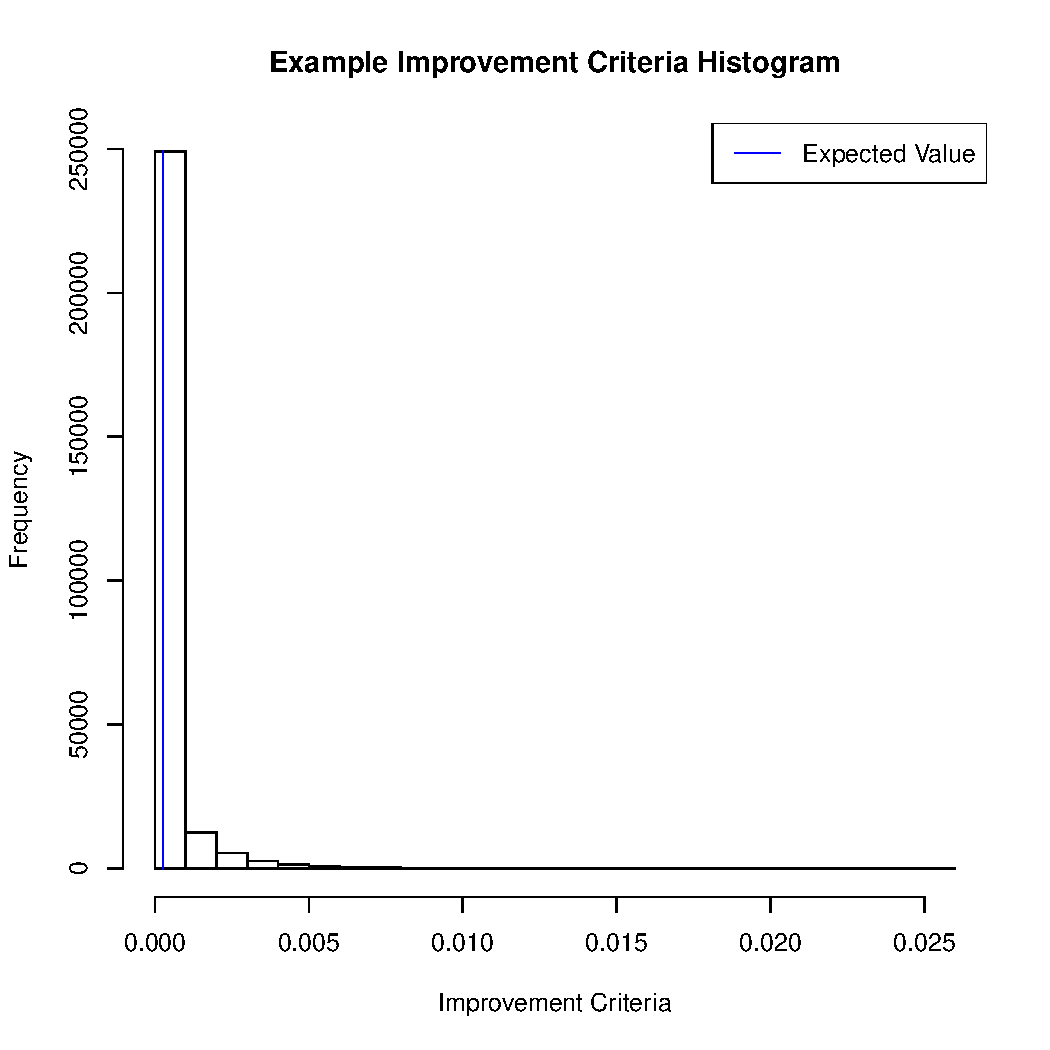
\includegraphics[width=0.5\textwidth]{./figures/exampleIHist.pdf}
	\end{center}
	\vspace{-0.85cm}
	\caption{An example $\ix$ sample histogram, demonstrating the extreme right skew. Additionally, $\Eix$ is shown in blue.}
	\label{IxEX}
	\end{wrapfigure}
	%
	%

	%
	The second major concern brought about by the application of SPC on EI is the distribution of $\ix$.
	%
	Upon investigation of this distribution it is quickly clear that $\ix$ typically follows a strongly right skewed distribution, due to the non-negative construction of the $\ix$ criterion.
	%
	This is not a fatal property of the distribution of $\ix$ in terms of the central limit theorem (CLT), although it does yield nearly worst case asymptotics in terms of the convergence of the sampling distribution to normality.
	%sampling method longer 
	A simple solution for getting more asymptotic results could include increasing the sample size of the draws of $\ix$.
	%
	However it is important to consider that by the nature of MCMC implementation of models like Model \ref{gpModel}, increasing the number of samples of $\ix$ entails taking more samples of every single parameter in the model.
	%
	Increasing the sample size of $\ix$ is a perfectly valid solution to this problem, if computation memory is of no concern, but it is not a particularly robust and satisfying solution.
	%
	Additionally, since the $\ix$ criterion is naturally bounded at 0, an unfettered normal distribution will always struggle to model the EI criterion since the normal distribution will never respect its boundary conditions.
	%
	Thus, modeling these data so as to find appropriate transformations to improve their asymptotics, and better model the boundary conditions of the problem, is a worthwhile consideration. 
	
	%
	%
	
	%
	In the following sections I address each of these concerns in turn. 
	%
	As I address each issue, I modify my method for tracking the information contained in the EI criterion so as to robustly identify convergence as inspired by SPC.

	\clearpage
	%
	%
% 	\subsubsection{Improved Normality}
	\subsection{Improved Normality}
	%
	%
	
	%
	%
	\begin{wrapfigure}{l}{0.5\textwidth}
	\vspace{-1.1cm}
	\begin{center}
	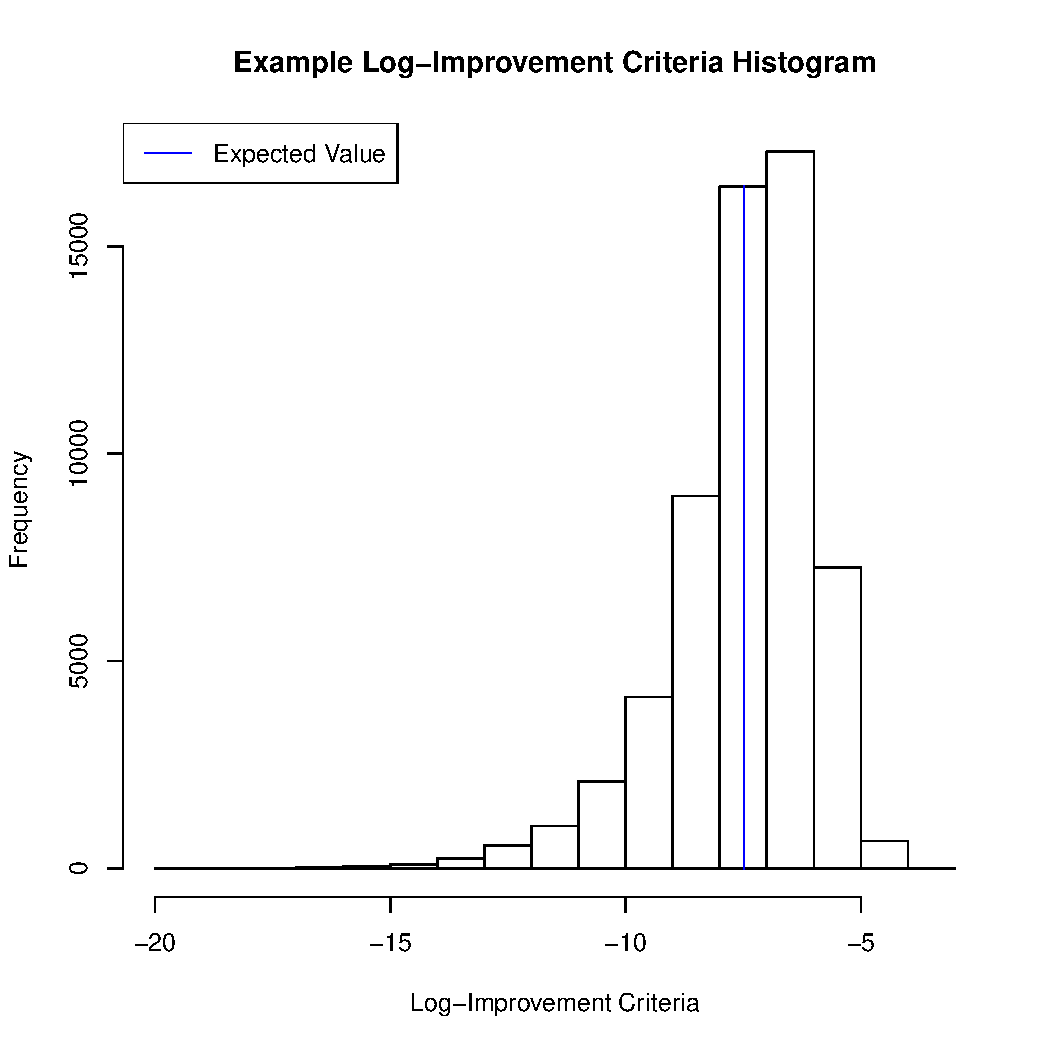
\includegraphics[width=0.5\textwidth]{./figures/exampleLogIHist.pdf}
	\end{center}
	\vspace{-0.85cm}
	\caption{An example $\log\ix$ sample histogram, demonstrating improved skew. Additionally, $\E{\log\ix}$ is shown in blue.}
	\label{logIxEX}
	\end{wrapfigure}
	%
	%
	
	%
	For the sake of improving the asymptotic convergence of the EI sampling distribution to normality it is of much desire to transform the distribution of $\ix$ so as to be less skewed.
	% of the form seen in figure \cite{IxEX}
	A simple and often effective transformation for getting skewed distributions to more resemble normality is a simple $\log$ transformation of the data.
	% 
	In this case simply log transforming the MCMC samples of the $\ix$ criterion is not always possible.
	%
	By the definition of the $\ix$ criterion, an $\ix$ sample can at its lowest take a value of 0; see Eq. (\ref{ix}).
	%
	MCMC samples that explore $\ix$ values as low as 0 will render the $\log$ function useless, as $\log$ is undefined for values $\le 0$.
	%
	Thus rather than actually transforming the data in this way, I propose modeling these samples with a log-normal distribution.
	
	%
	Recall that if a random variable $X\sim Log$-$N(\mu, \sigma^2)$, then another random variable $Y=\log(X)$ is distributed $Y\sim N(\mu, \sigma^2)$.
	%
	Furthermore, if $m$ and $v$ are, respectively, the mean and variance of a log-normal sample, then the mean, $\mu$, and variance, $\sigma^2$, of the associated normal distribution are given by the following relation,
	%
	\begin{eqnarray}
	\mu = \ln\left( \frac{m^2}{\sqrt{v+m^2}} \right) &~&  \sigma^2 = \ln\bigg( 1+ \frac{v}{m^2} \bigg).
	\label{lnRelate}
	\end{eqnarray}
	%
	Using this relation we do not need to transform any of the $\ix$ samples; we can instead jump straight to the mean of the samples that would have resulted from transforming these $\ix$ samples.
	%
	That is to say, by using relation \ref{lnRelate} we immediately get a value for $\E{\log\ix}$ without actually taking the log of $\ix$ samples.
	%rather than
	Considering the distribution of $\log\ix$, seen in figure \ref{logIxEX}, the asymptotics ensuring the normality of the distribution of $\E{\log\ix}$ as compared with that of $\E{\ix}$ are far favorable. % the distribution of  are far favorable to those present necessary for the CLT will be are must more  to work its magic will be ever in our favor through considering the $\E{\log\ix}$ as compared with the standard EI criteria.
	
% 	\clearpage
	%
	%
	\subsection{Exponentially Weighted Moving Average}
	%
	%
	
	%{\color{red}EWMA (time series concepts) for added robustness }
	%
	In general moving average methods use the idea of a rolling average to smooth data that arrive as a series. % techniques for smoothing data that arrive as a series. %, just as is the case for EI values in our optimization routine.
	%weighted I not only want to smooth the data, but the calculation of
	EWMA methods achieve this smoothing by assigning exponentially decreasing weights to successive points in a rolling average among all of the points of a series. 
	%so as to focus the attention of the moving average on recent 
	%For application of EWMA on EI progression the smoothing behavior since the EI values can display I am really interested in weighting the values such that more recently observed values are more heavily considered in the moving average.
	%
	%Exponentially Weighted Moving Averages (EWMA) precisely achieves this goal by assigning exponentially decreasing weights to each point in the series.
	%moving
	This disproportionately focuses the attention of the moving average on recent information (i.e. the most relevant information in this case), while still smoothing the overall series progression with at least some memory of past values. % giving some weight some memory.  
	%%our wild adosecence.focusing our attention on the most relevant, recent, information an display incensed variability and a decreasing trending pattern
	These properties of the EWMA have shown to provide a robust solution for tracking the progression of means that are subject to subtle drifting processes \cite{adaptEWMA}, such as one might expect to see in convergence.
% 	%
% 	For application of EWMA on EI progression
% 	Together these properties of the EWMA have the effect of focusing provide a good candidate for monitoring the convergence of EI.
% 	%
% 	Since after its initial naive fluctuations, the EI values tend to subtly shift from the early wild fluctuations of pre-convergence   
% 	since often EI values tend to slowly  as one might expect for the behavior of convergence.
	%
	
	%
	
	%the exponentially decreasing weights of tracking the EI values via EWMA in reverse order has the overall effect of
	Since early $\E{\log\ix}$ values generally behave differently than later values, I use the EWMA procedure to track the progression of $\E{\log\ix}$ values in reverse order.
	%current 
	This has the effect of forgiving the wild fluctuations of early inexperienced explorations and highlighting the most recent experiences with $f$. %current values of EI.
	%
	Furthermore, the exponentially decreasing weights are well suited for monitoring convergence in this case because they have the ability to smooth out the initial EI fluctuations, while still having the resolution to pick out the subtle shifts inherent to the convergence process.
	%since after the initial period of naive fluctuations the EI progression tends to subtly slide into convergence, the ability of EWMA to smooth out the initial fluctuations while still picking up on the subtle shifts inherent to convergence makes EWMA a good method for identifying convergence in this case. 
	%
	Further dynamics of EWMA are well explained by Box et al. \cite{boxBook}; additionally EWMA charts, among other common control charts, can easily be implemented in R by using the R package \verb|qcc| \cite{qccPack}.

	%
	%
	
	%
	If $Y_i$ is the current value of $\E{\log\ix}$, and $Z_i$ is the EWMA statistic associated with this current value, then the initial value $Z_0$ is set to $Y_0$ and for $i>0$ the EWMA statistic is expressed as,
	%
	\begin{equation}
	Z_i=\lambda Y_i+(1-\lambda)Z_{i-1}.
	\label{ewmaStat}
	\end{equation}
	%
	Above, $\lambda$ is a parameter that defines the weight $\left( \text{i.e. }0<\lambda\le1\right)$ assigned to the most recent observation, $Y_i$.
	%Eq. (\ref{ewmaStat})
	The recursive expression of the statistic ensures that all subsequent weights geometrically decrease as moving back through the series.
	
	%
	%
	
	%
	Typically values of $\lambda$ range from $0.1\le\lambda\le0.3$, with a default value of $\lambda=0.2$, as described by Box et al. \cite{boxBook}.
	%
	Additionally Box et al. explains how to estimate a $\hat\lambda$ so as to minimize sum of squared deviation of the forcasting errrors ($S_\lambda$) of the resulting EWMA series. %  data specific $\hat\lambda$ value by minimizing the sum of squared deviations with respect to $\lambda$. % , thus tailored for each particular data set.
	%the more quickly
	In general large values of $\lambda$ assign more weight to recently observed values, and thus past observations effect the moving average less. %  on the moving average quickly forgets about past observations.
	%
	Conversely, small values of $\lambda$ assign less weight to recent observations, and thus small values of $\lambda$ provide more smoothing across the effects of past observations. 
	%provide better sensitivity $\E{\log\ix}$
	Hence larger values of $\lambda$ tend to be better suited for dealing with large shifts, and small values of $\lambda$ are more sensitive to small shifts.
	%
	Often it is the case with EWMA that the best choice of $\lambda$ is based on ``expert opinions'' related to the underlying data generating process.
	%the choice of an appropriate $\lambda$ requires an
	For identifying convergence, ``expert opinions'' come in the form of an in-depth understanding of how EI values behave relative to the specific search phenomena related to the expected behavior of $f$.
	%Hence larger values of $\lambda$ tend to be better suited for dealing with the large EI shifts associated with uncertain mean predictive surfaces.
	%In contrast, small values of $\lambda$ are more sensitive to small EI shifts, and thus are well suited for identifying convergence when the
	
	%
	%Most reasonable values for $\lambda$ provide decent results, thus for simplicity I focus on the default case of $\lambda=0.2$ in all of my examples. 
	
	%
	%
	
	%how the plot In order to identify convergence
	For identifying convergence it is also important to define the control limits on the statistic seen in Eq. (\ref{ewmaStat}).
	%
	Again, this amounts to considering an interval on the sampling distribution of interest.
	%, under the assumptions that the $Y_i$ arrive as $i.i.d.$ samples
	In this case we are interested in the sampling distribution of the $Z_i$, if the $Y_i$ are $i.i.d.$ then Lucas and Saccucci \cite{ewmaPaper}  show that we can write $\sigma^2_{Z_i}$ in terms of $\sigma^2_{Y}$. %, Lucas and Saccucci \cite{ewmaPaper}  show,
	%
	\begin{equation}
	\sigma^2_{Z_i} = \sigma^2_{Y}\left(\frac{\lambda}{2-\lambda}\right)\left[1-(1-\lambda)^{2i}\right]
	\end{equation}
	%\substack{i.i.d.\\\sim}
	Thus if the $Y_i \stackrel{i.i.d.}{\sim} N\left(\mu, \frac{\sigma^2}{n}\right)$ the sampling distribution for $Z_i$ is $Z_i \sim N\left(\mu, \sigma^2_{Z_i}\right)$.
	%
	Furthermore if we choose a confidence level through a choice of the constant $c$, the control limits based on this sampling distribution are seen in Eq. (\ref{EWMACL}).% follow on the next page.
	
	%
	%\begin{figure}
	%\vspace{-1cm}
	\begin{eqnarray}
	\text{CL}_i &=& \mu \pm c \sigma_{Z_i}\nonumber\\
	&=&  \mu \pm c ~ \frac{\sigma}{\sqrt{n}}~\sqrt{\left(\frac{\lambda}{2-\lambda}\right)\left[1-(1-\lambda)^{2i}\right]}
	\label{EWMACL}
	\end{eqnarray}
	%\end{figure}
	%
	
	$~$\\\\
	Notice that since $\sigma^2_{Z_i}$ has a dependence on $i$, the control limits do as well.
	%the focusing effect of EWMA. % this focusing effect.
	Looking back through the series brings us away from the focus of the moving average, at $i$, and thus the control limits widen when traversing backwards through the series resulting directly from the geometrically decreasing weights.  
	%
	
	%
	%
	
	%
	At this point it is necessary to take a step back from the modeling details and motivate the use of such models on the real $\E{\log\ix}$ behavior.
	%
	At first glance it is not clear that the $Y_i$ are in fact $i.i.d$. % throughout the entire progression of values. % \stackrel{i.i.d.}{\sim} N\left(\mu, \frac{\sigma^2}{n}\right)$.
	% thus making the $i.i.d.$ assumption appropriate.
	Indeed the early iterations of the process certainly do not display $i.i.d.$ looking $Y_i$ values.
	%
	However once the process proceeds far enough, the $Y_i$ enter a state of control; thus for the values that are in control, the $i.i.d.$ assumption is very reasonable.
	%identifies the
	The fact that the pre-convergence $Y_i$ do not necessarily demonstrate control may in large part have to do with their lack of $i.i.d.$ness, and thus identifying control in this way validates the appropriateness of this model by identifying control. % in which the notion of $i.i.d.$ness is implied.
	%
	That is to say, in this application the concept of $i.i.d$ samples serves as part of the check for control; realizing control validates the assumption of $i.i.d.$ samples and vice versa.
	%be due to their identification as  prior to reaching control do not require  Prior to reaching control 
	%The notion of control implies some Inherent to the idea of control is the idea that the process is $i.i.d.$ 
	%
	%The particular interest for the accuracy of this model surrounds the identification of convergence, and since the $Y_i$ presumably enter a state of control at convergence and convergence requires a reasonable $i.i.d$ assumption the idea is that when it really matters   
	%and furthermore, the $\ix$ criteria suffers from a strong right skew.
	
	%
	%
	
	%
	Another detail worth further recognition, is the asymptotics on which all of the this logic is built.
	%Let us not forget that, e
	Even after log transformation of the $\Eix$ criterion, $\E{\log\ix}$ is still only asymptotically normal.
	%
	Even though the distribution of $\E{\log\ix}$ is likely to be quite normal, via the CLT, it is still worth mentioning that any non-normality left in the model is left for EWMA's own robustness to cope with. 
% 	In section 2.2 I address a modeling consideration that should drastically improve the assumption of normality on the $Y_i$. % %in this case.
	%
	Furthermore, constructing a robust model for identifying convergence is of primary concern, especially considering the many varied conditions this model must perform under.
	%
	In considerations of this type, Box et al. \cite{boxBook} argues that EWMA is a robust and parsimonious solution in many cases, especially with respect to disputes in the distribution and stationarity of the $Y_i$.
	% and provide accurate results in many situations
	Thus the EWMA logic should provide the sturdy and robust framework necessary for dealing with data of \mbox{this type.}  
 
	
% 	%
% 	%
% 	\subsection{Additional Modeling Considerations}
% 	%
% 	%
	
	%
	%
% 	\subsubsection{The Control Window}
	\subsection{The Control Window}
	%
	%
	
	%
	%However, there are some issues in the application of a naive
	%
% 	One additional feature is necessary to adapt to typical SPC philosophy so as to identify convergence.
	%
	Typically in SPC some initial number of samples are gathered and deeply investigated to establish an initial standard for control that is not wildly off-base.
	%
	Investigation in this setting amounts to careful analysis of the conditions related to points that fall beyond the control limits; often with the intention of attributing some deterministic reason for the lack of control.
	%
	Observations investigated in this way are often discarded from the calculation of initial control limits because they are found not to represent the desired state of control, and thus through their exclusion the standard for control is elevated.
	
	% 
	In the setting of optimization it is not desirable to study each pass of our routine so carefully, and often such analysis would not be meaningful.
	%
	However, for the sake of keeping in the spirit of SPC, as well as other practicalities, I offer a compromise that frames the setting for which convergence is to be identified.
	%
	I propose the idea of a sliding window of fixed size, $w$, that I call the {\it control window}.
	%is to be  all be the sole provider of information for the calculation of control limits.in the calculation of
	The idea being, only information from the $w$ points currently residing inside the control window is used to calculate the control limits, but the EWMA statistic is still computed for all values as before.
	%contribute information toward
	%The EWMA statistic shall be computed for all values, but only a set number, say $w$ of the values, shall reside inside the control window at any given time, and thus only these $w$ values are included in the construction of control limits.
	%
% 	Since 
	%, so as to fill the control window
	Initially, I allow the algorithm to fill the control window, by collecting $w$ observations of $f$.
	%;
	As new observations of $f$ arrive, the oldest value is removed from the control window, thus allowing for the inclusion of a new value.
	%\singlespacing
	This offers an automated way of basing the standard for convergence only on the most updated and relevant information.
	%
% 	Furthermore since at convergence we only require control inside the control window, basing the control limits solely on information for the  validated the necessary $i.i.d$ assumption in constructing the control limits.
	
	%
	%
	
	%The size of this window is left up to the discretion of user,.
	The size, $w$, of the control window is important for correctly identifying convergence.
	%
	Because $w$ may vary from problem to problem it is ultimately left as a tuning parameter of the system.
	%
	Choosing the correct value of $w$ presents an interesting decision problem since underestimating the size of the control window may lead to premature convergence, but if $w$ is too large, we compute unnecessary objective function evaluations.
	%It is t
	Thus it may be important to consider these two opposing forces when choosing an appropriate value for $w$.
	%
	I recommend conservatively large values for $w$ because I regard premature convergence to be a greater problem than extraneous function evaluations.
	%
	As a default value $w=30$ has provided me a reasonable starting point for further analysis.
	%
	I have found that choosing $w$ based on the value of $\lambda$ seems to be an efficient way of tuning $w$.
	%
	As a general trend, the larger the value of $\lambda$, the more fluctuation present in the EWMA statistic.
	%% the fluctuations in the EWMA statistic. %Conversely for small $\lambda$, smaller values of $w$ are acceptable. are necessary allow averages over more elements of the  to  average out ; fluctuations 
	Thus for good results, large $\lambda$, naturally imply large values of $w$ for an accurate representation of the increased fluctuations of the EWMA statistic in the repeated sampling average.
	%due to decreased fluctuations in the EWMA statistic
	Conversely for small $\lambda$, smaller values of $w$ are acceptable.
	
	%
	%Although it would be interesting to carefully study the loss associated with each case based on the time and resources necessary in practice.

% 	\clearpage
	%
	%
	\subsection{EWMA Convergence Chart}
	%
	%
	
	%
	Recall that this work is meant to apply at step 7) of figure \ref{procedure}.
	%
	Thus, at each iteration we can obtain a new $\E{\log\ix}$ value to track via the EWMA procedure outlined in Section 2.2.
	%
	If we then apply the control window to this EWMA tracking procedure, interesting rules for identifying convergence naturally arise. 
	
% 	{\raggedright

	%triggers an out-of-control state when a $Z_i$ value exceeds the established control limits.
	The typical EWMA identifies out-of-control observations  by simply identifying which $Z_i$ values exceed the established control limits. This may be adequate for a check of simple

% 	}
	% 	\clearpage
	%
	%
	\begin{wrapfigure}{l}{0.5\textwidth}
	\vspace{-1.1cm}
	\begin{center}
	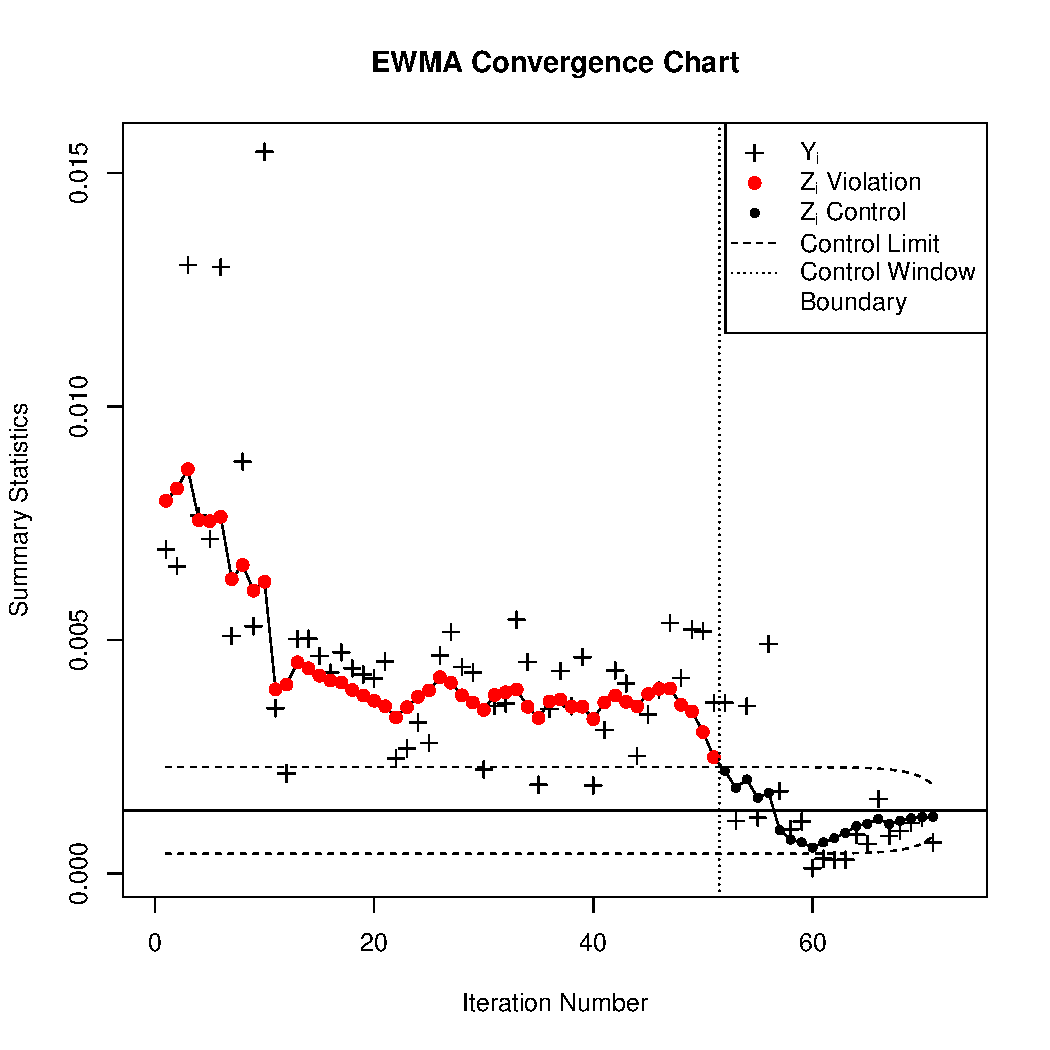
\includegraphics[width=0.47\textwidth]{./figures/exampleEWMA.pdf}
	\end{center}
	\vspace{-0.85cm}
	\caption{An example EWMA convergence chart based on the fabricated EI progression in figure \ref{EIxEX}. This chart is converged.}%has identified convergence. }
	\label{EXconverge}
	\end{wrapfigure}
	%
	%
	%

	%This may be adequate for a check of simple
	\noindent control, but is not a stringent enough standard for determining convergence.
	%converged state to be in control
	In identifying convergence we not only desire that the converged state has reached a state of control, but we also desire a state of control that indicates significantly lower expectations for finding new minima in the future.
	%
	This suggest a dual use of the the control window in suggesting convergence.
	%% that they define.
	Firstly, I require that all $Z_i$ values inside the control window fall within the control limits. 
	%the past (i.e.. outside the control window)
	Secondly, since we wish to indicate a move from the initial pre-converged state of the system, I require at least one point from beyond the control window to fall outside the defined control limits.
	%the intersection of
	A set of $Z_i$ satisfying both of these conditions indicate the desired state of convergence.
	%
	Satisfying only one of these conditions indicates insufficient exploration of the objective landscape and thus further iterations of procedure \ref{procedure} are required.
	
	%is a type of moving control. , thus sliding
	Together these rules capture the notion that the process of convergence is a slide from a pre-convergence state, into a converged state of control. 
	%recent values of $Z_i$ (i.e.
	In the converged state, $Z_i$ values in the control window (i.e. recent values) indicate control in the classical sense.
	% so as to identify convergence.it provides a way to express the idea of moving control,Additionally, s
	Since the control window partitions the $Z_i$ into new and old values, the control window provides a mechanism for identifying when control has shifted into a state of control that has moved sufficiently from the initial pre-convergence state.
	%
	These added considerations for the behavior of current $Z_i$ values, relative to old observations, differentiate the classical notion of control charts from what I call a convergence chart.  
	
	
%
%
\section{Examples}
%
%

%%of monitoring convergence via the above described EWMA convergence chart.
In this section I provide a series of test function examples, as well as a case study demonstrating the use of the EWMA convergence chart for monitoring convergence.
%a strategy - or - strategies
The test function examples are meant to highlight strategies for tuning $\lambda$ and $w$ relative to the observed behavior of $f$, as well as demonstrate various states of convergence with respect to various objective function behaviors.
%
Additionally, I consider the Lockwood pump-and-treat case study as a practical example of how the EWMA convergence chart may be used in less tidy optimization problems.
% %
% {\color{red}
% Additionally, I consider the Lockwood pump and treat case study... %to show how the EWMA chart may be used in real optimizations settings.
% }
	
	\clearpage
	%
	%
	\subsection{Rosenbrock}
	%
	%
	
	\begin{figure}[!h]%{l}{1.\textwidth}
	\centering
	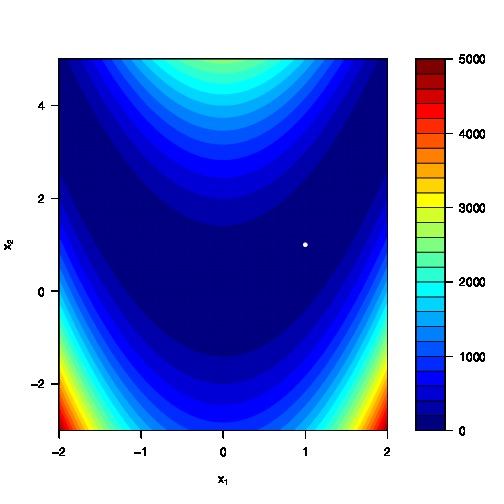
\includegraphics[width=0.49\textwidth]{./figures/roseContour.jpg}
	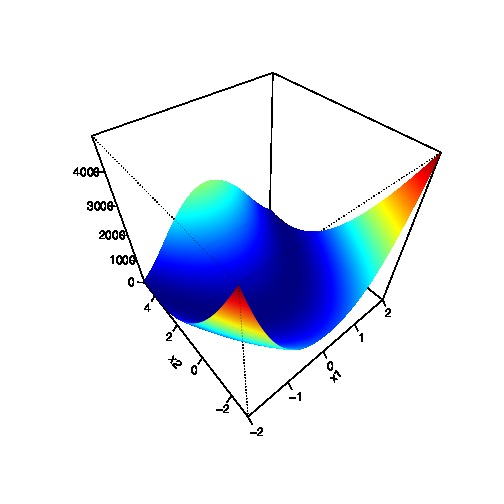
\includegraphics[width=0.49\textwidth]{./figures/rosePersp.jpg}
	\begin{eqnarray}
	f(x_1, x_2) &=& 100\left(x_2-x_1^2\right)^2 + (1-x_1)^2 \\
	\text{Minimum}&:& f(1, 1)=0\nonumber
	\end{eqnarray}	
	\end{figure}
	
	%banana-shaped
	The Rosenbrock function \cite{rosePaper} is a classic optimization benchmark, and thus it is only fitting to begin with an analysis of its long and narrow, flat parabolic valley.
	%
	Exploring the banana-shaped valley is an exercise in self control, as the flat valley floor seems to endlessly meander around the curve of the banana with relatively little descent as compared with the steep $4^{th}$ order polynomial valley walls.   
	%% of the valley.
	This stark difference in scale tempts optimization routines to prematurely claim convergence all along the lengthy valley floor. 
	%% just above and to the right of the vertex of the parabolic valley.
	As indicated above, the true global minimum value is attained jarringly off centered at (1, 1), where the objective value eventually falls to 0. 
	
	%above pictured % , with of the Rosenbrock function,
	For the sake of this analysis I focus on the pictured intervals, in this example I am focusing on Rosenbrock with \mbox{$-2\le x_1\le2$}; \mbox{$-3\le x_2\le5$}.
	%(i.e. \mbox{$-2\le x_1\le2$} and \mbox{$-3\le x_2\le5$}) %% The pictured interval% we ... the model
	This interval subjects the surrogate model to the flat valley floor, but since we start optimization with a naively chosen $\bm{X}$,  initially the model is forced to make some consideration of the steep valley walls.
	
	%
	%surrogate model of the surrogate modeling procedure.
	\begin{wrapfigure}{l}{0.5\textwidth}
	\vspace{-1.1cm}
	\hspace{-1cm}
	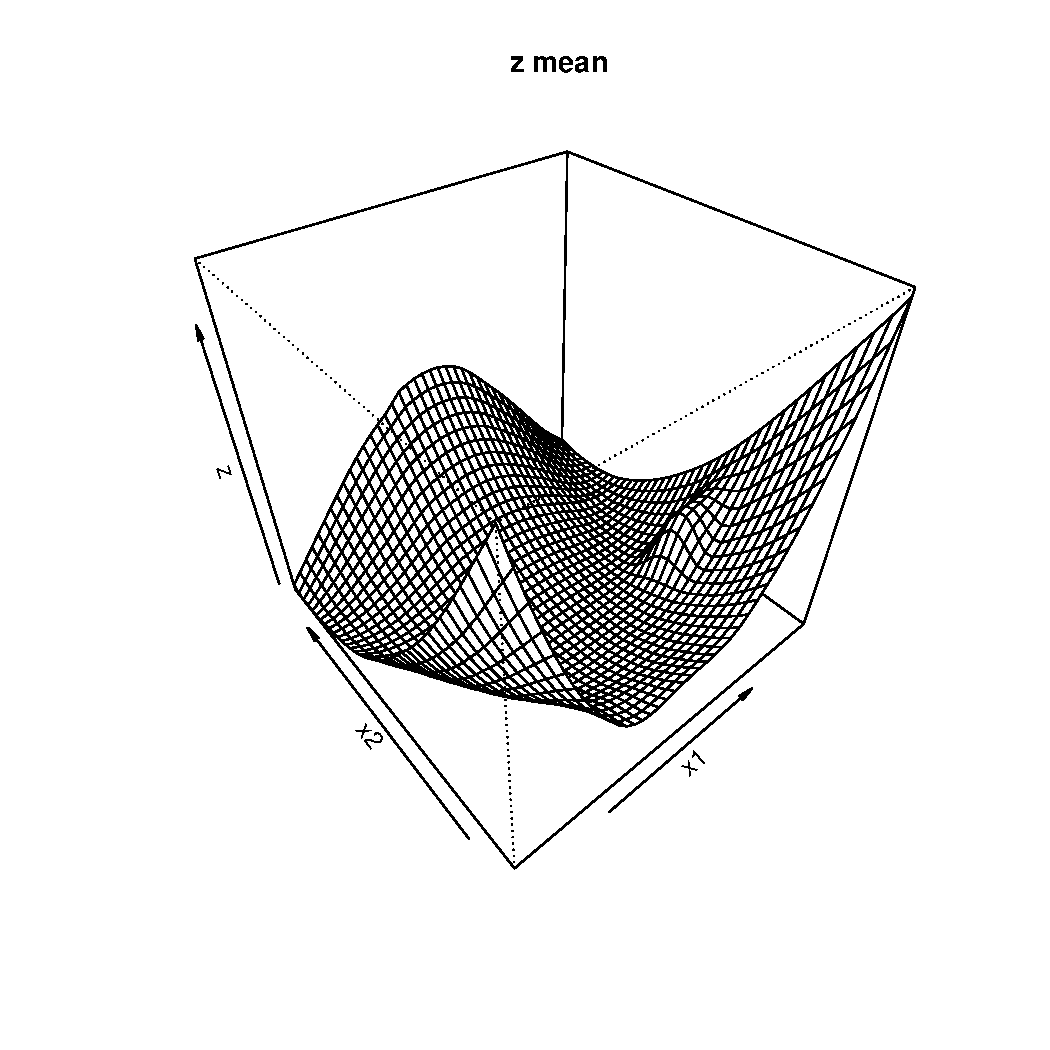
\includegraphics[width=0.6\textwidth]{./figures/gpMeanRosegpPic.pdf}
	\vspace{-2.5cm}
	\caption{The GP mean predictive surface of the Rosenbrock function after 70 iterations. }
	\label{roseGP}
	\end{wrapfigure}
	%
	%
	%
	\noindent
	As optimization, proceeds only the maximum EI candidate location is added to $\bm{X}$, and thus for the sake of optimization no time is wasted searching for a minimum in the steep walls. % we don't  
	%we gather more and more 
	Furthermore, since the maximum EI candidate location typically falls somewhere in the valley floor, more and more points from inside the valley are gathered.
	%surrounding valley walls
	This forms a very good model for what the true shape of the Rosenbrock function looks like inside this valley, but gives only the necessary impression of the surrounding walls needed to identify that they do not contain minima, as seen in Figure (\ref{roseGP}).
	%
	
	%
	%
	
	%% with respect to GP surrogate model optimization. example demonstrates a very typical case typical case  for identifying convergence.
	Since the Rosenbrock function is not highly multimodal and does not contain any hard to discover features, it provides an example of the kind of function that will provide the default EI behavior.  
	%
	%Thus this represents a default setting for choosing values of the tuning parameters $\lambda$ and $w$.
	%
	The basic strategy for tuning $\lambda$ and $w$ starts by first choosing a value for $\lambda$, to remove a degree of freedom from the system. %, by choosing a value for $\lambda$.
	%
	Since Rosenbrock provides an example of default convergence behavior, the default $\lambda$ value is appropriate, $\lambda=0.2$.
	%easily
	After choosing $\lambda$, the choice of $w$ can be made based on the chosen value of $\lambda$.
	%
	Again since $\lambda$ was chosen in accordance with the default value, the default value of $w=30$ is also appropriate here.

	%identifying convergence 
	Recall that for constructing an EWMA convergence chart it is necessary to first fill the control window so as to establish some initial opinion of the searching process.
	%
	\mbox{Figure (\ref{roseEWMAStart}, {\it left})} shows this initial, pre-convergence state, for the Rosenbrock function as described thus far.
	
	\clearpage
	%
	%
	\begin{wrapfigure}{l}{0.5\textwidth}
	%\hspace{-1cm}
	\vspace{-0.2cm}
	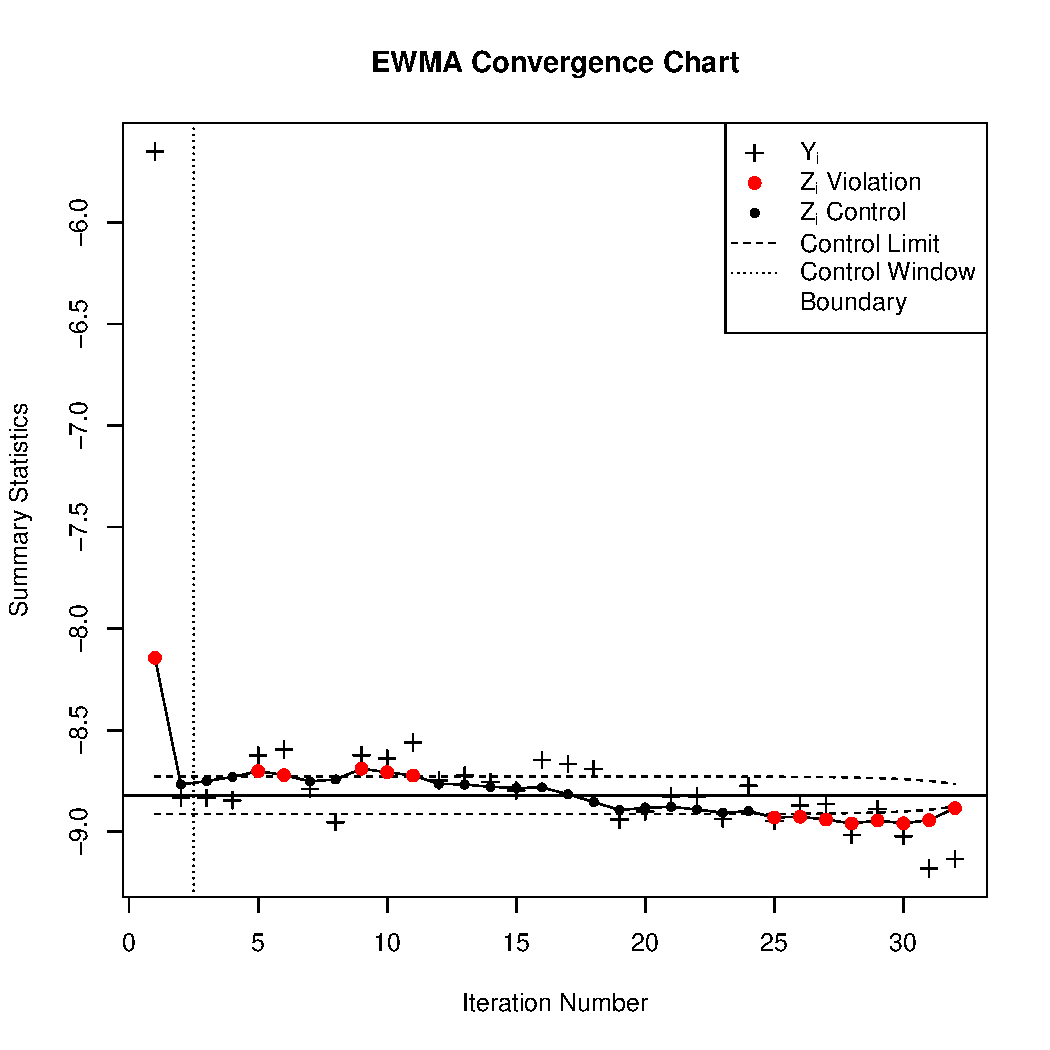
\includegraphics[width=0.245\textwidth]{./figures/ewmaConvChartRoseEasyEasyStart.pdf}
	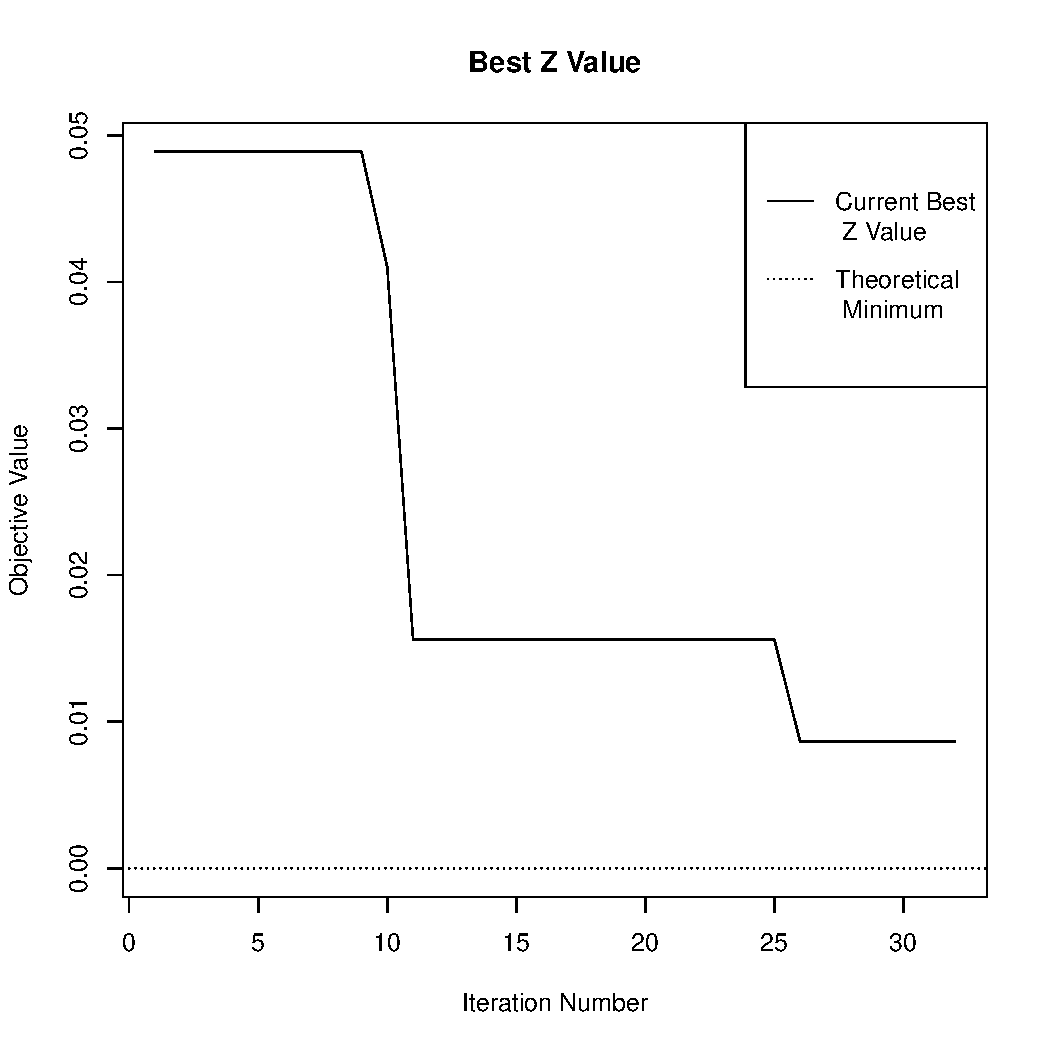
\includegraphics[width=0.245\textwidth]{./figures/bestZRoseEasyEasyStart.pdf}
% 	%\hspace{-1cm}
% 	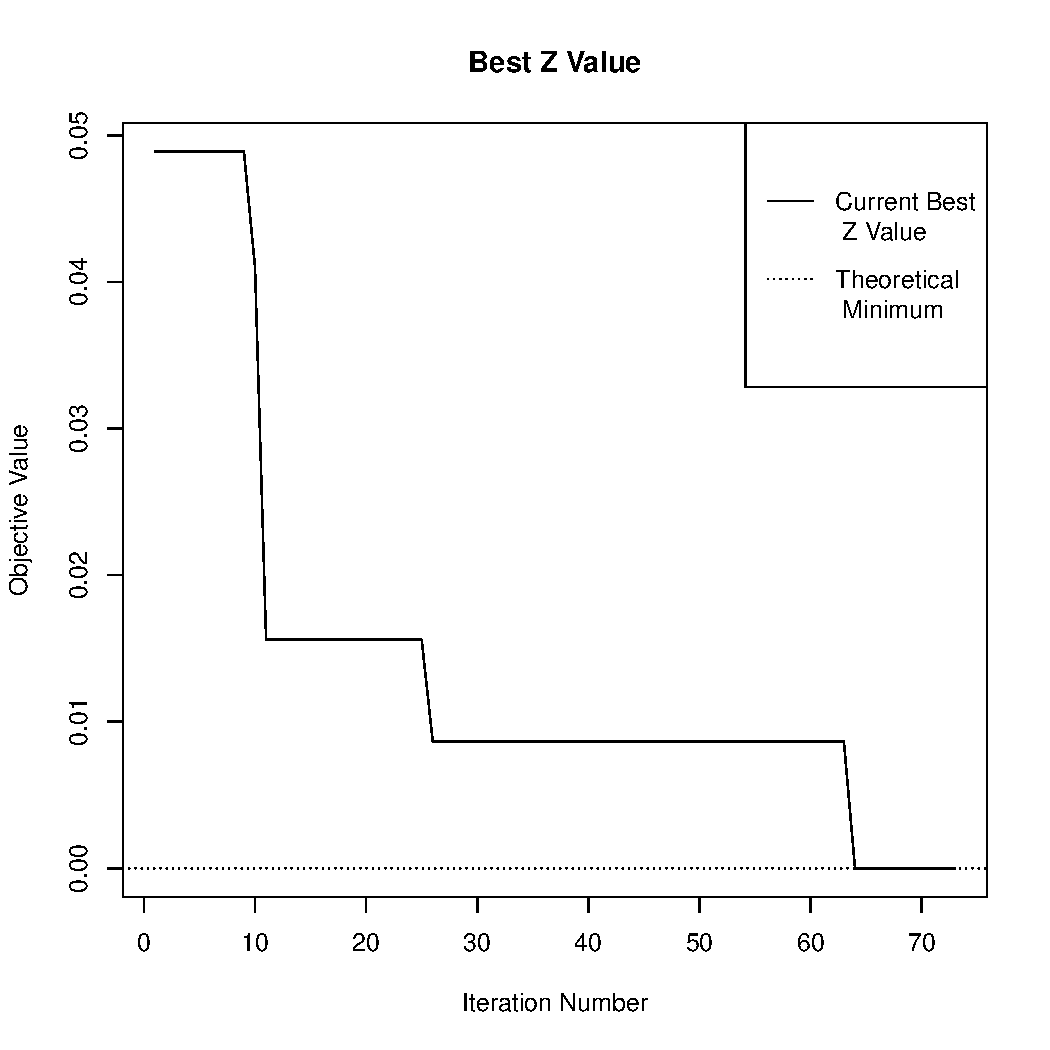
\includegraphics[width=0.245\textwidth]{./figures/bestZRoseEasyEasyEnd.pdf}
% 	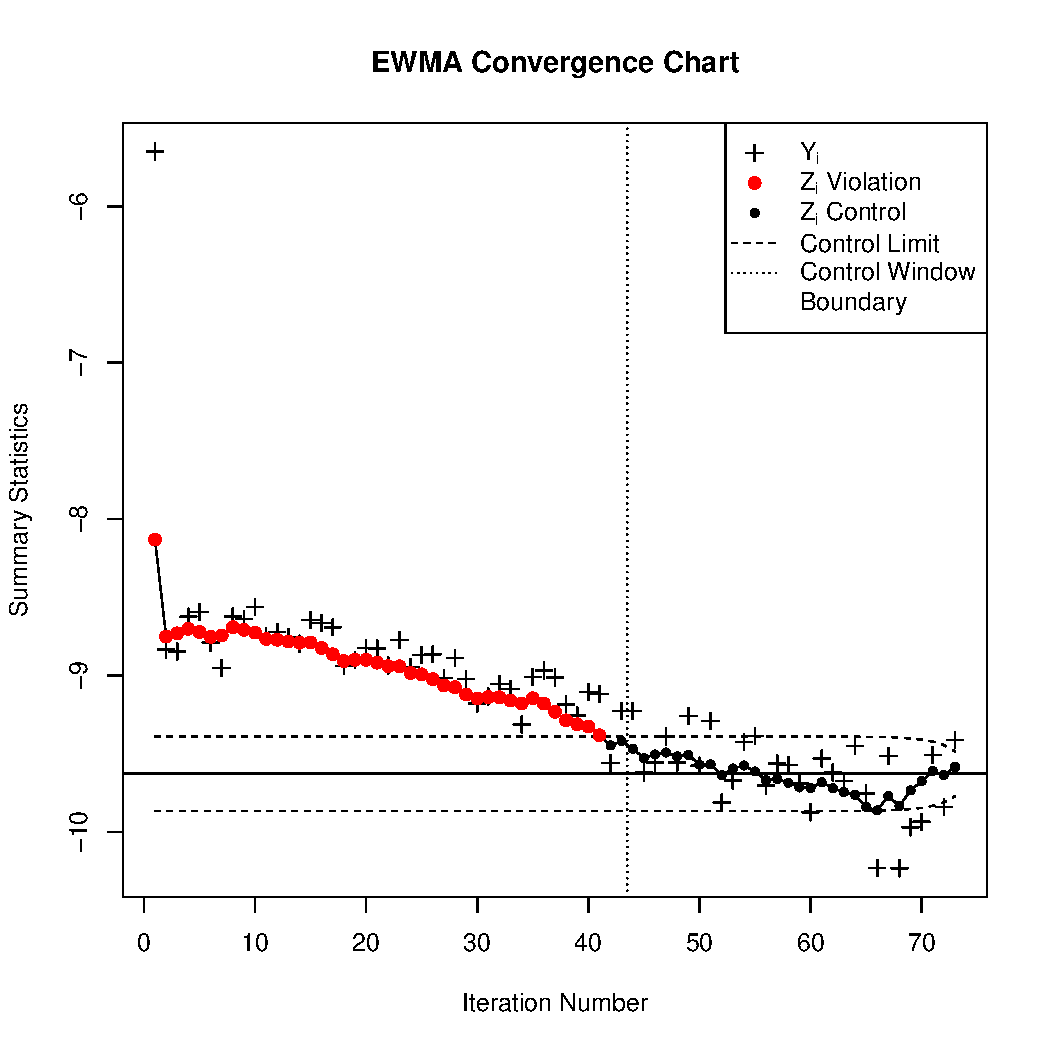
\includegraphics[width=0.245\textwidth]{./figures/ewmaConvChartRoseEasyEasyEnd.pdf}
	% for Rosenbrock
	\caption{({\it left}) The initial pre-converged state of the EWMA convergence chart. ({\it right}) The cumulative smallest objective function value at each iteration.}
	\label{roseEWMAStart}
	\end{wrapfigure}
	%
	%. 
	%
	\noindent
	The EWMA convergence chart shows an out-of-control state in the control window, with violations of the upper control limit for older values and violations of the lower control limit for more recently observed values.
	%
	This pattern indicates that the $\E{\log\ix}$ values are still in a steady decreasing state, and more iterations of the optimization procedure are required.
	%
	As the optimization procedure is allowed to proceed these violations move out of the control window and eventually a set of $\E{\log\ix}$ values fill the control window which do not display any violations inside the control window, as seen in Figure (\ref{roseEWMAEnd}, {\it left}).
	%
	Furthermore Figure (\ref{roseEWMAEnd}, {\it left}) demonstrates convergence because virtually all of the values beyond the control window violate the upper control limit.
	%
	
	%as optimization proceeds.
	As a check of the accuracy of the EWMA convergence chart, the right panels of both \mbox{Figures (\ref{roseEWMAStart}) and (\ref{roseEWMAEnd})} track the smallest objective function evaluation observed. 
	%
	\begin{wrapfigure}{l}{0.5\textwidth}
	%\hspace{-1cm}
% 	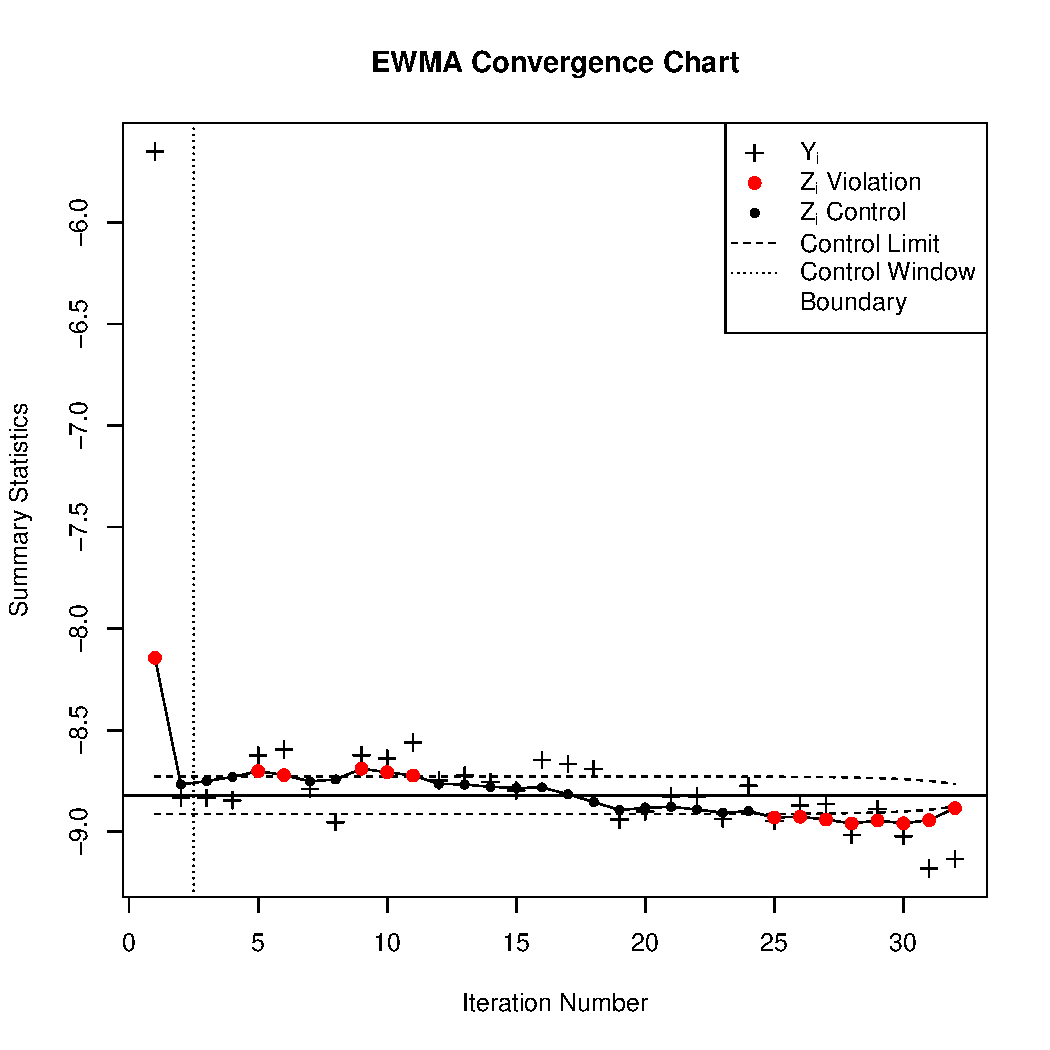
\includegraphics[width=0.245\textwidth]{./figures/ewmaConvChartRoseEasyEasyStart.pdf}
% 	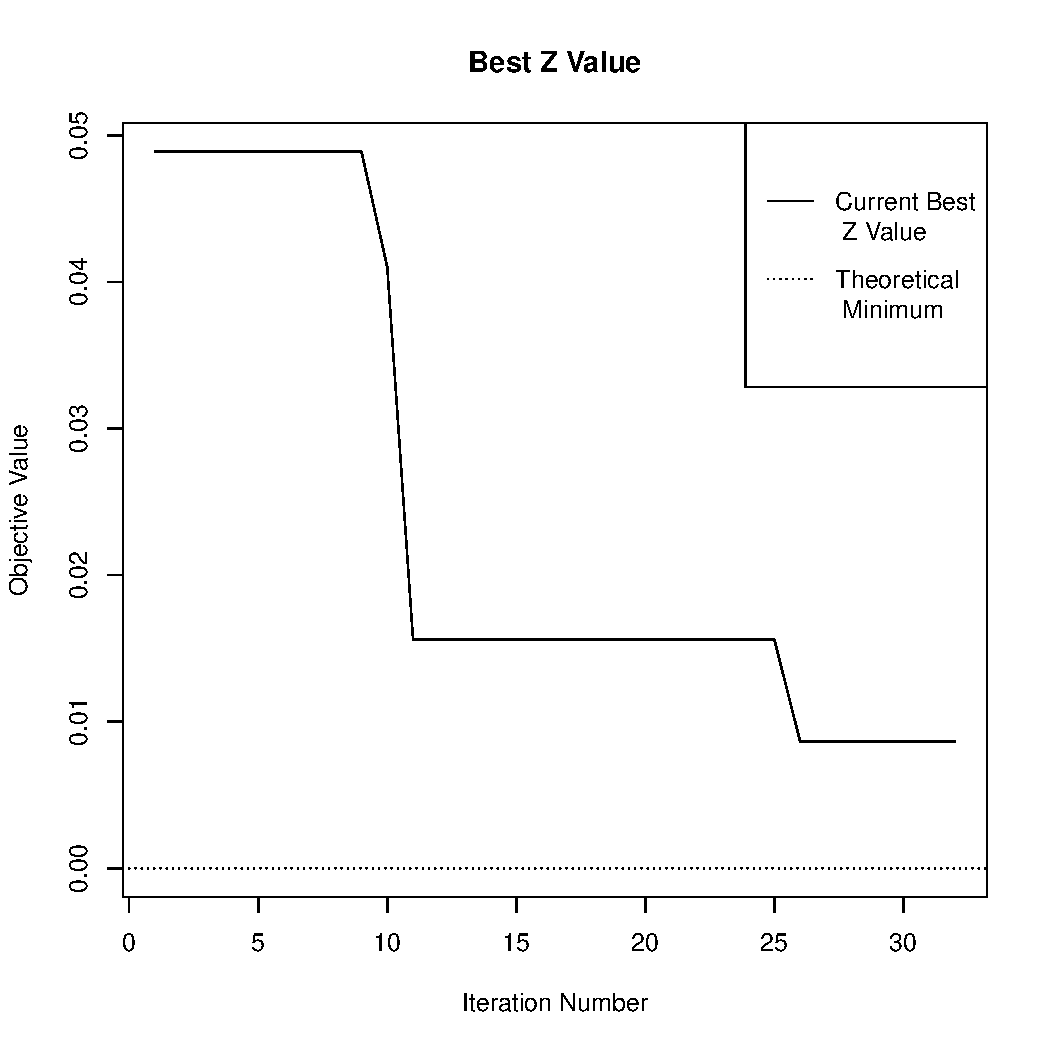
\includegraphics[width=0.245\textwidth]{./figures/bestZRoseEasyEasyStart.pdf}
% 	%\hspace{-1cm}
	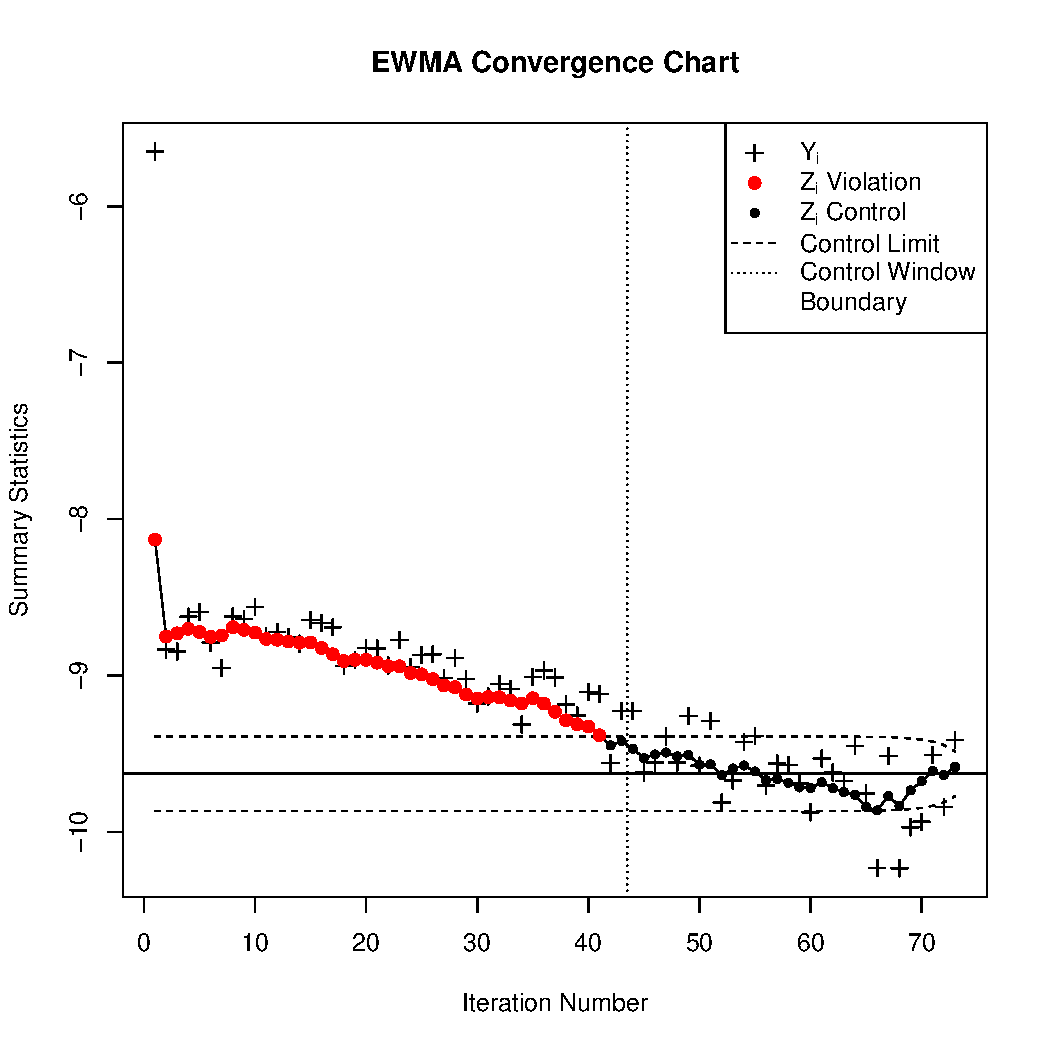
\includegraphics[width=0.245\textwidth]{./figures/ewmaConvChartRoseEasyEasyEnd.pdf}
	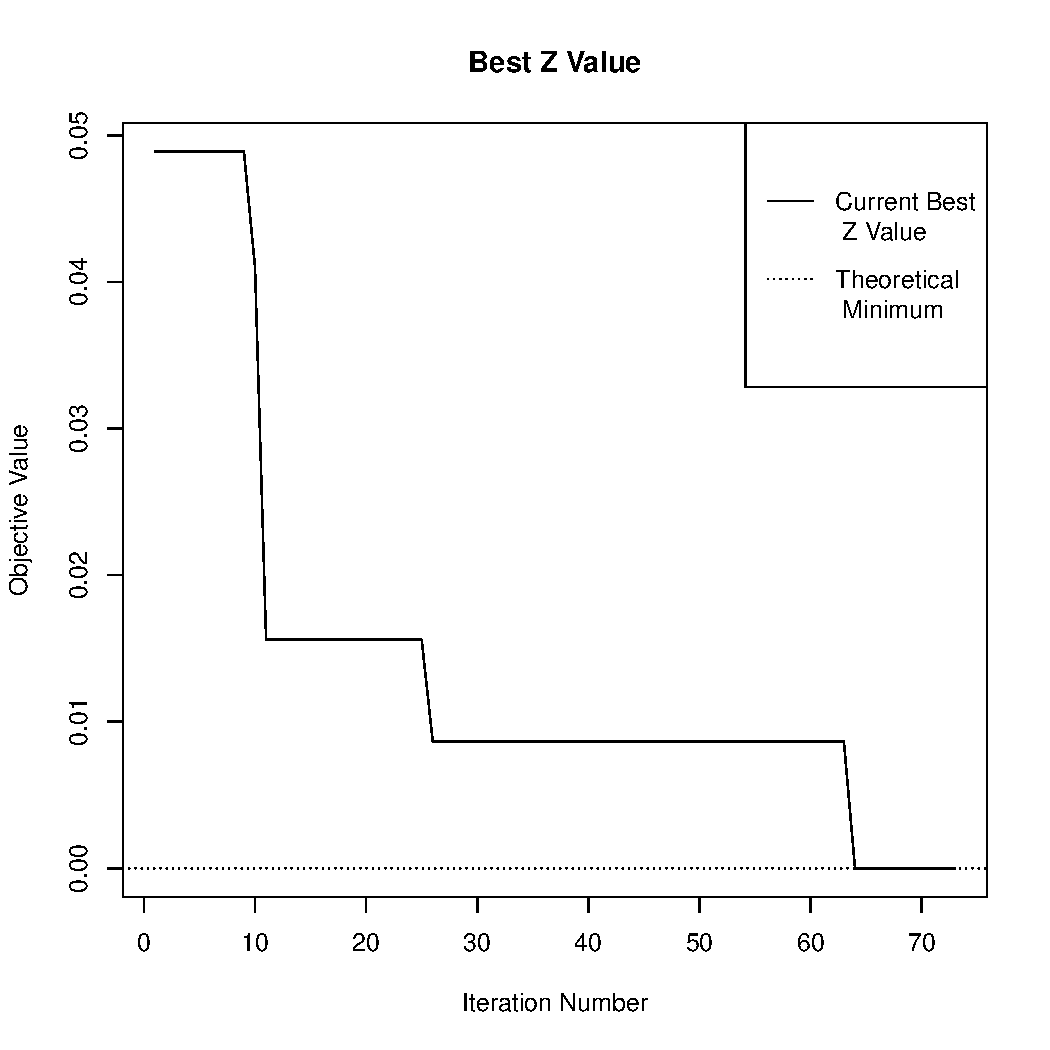
\includegraphics[width=0.245\textwidth]{./figures/bestZRoseEasyEasyEnd.pdf}
	% for Rosenbrock
	\caption{({\it left}) The converged state of the EWMA convergence chart. ({\it right}) The cumulative smallest objective function value at each iteration.}
	\label{roseEWMAEnd}
	\end{wrapfigure}
	% 
	Notice that in Figure (\ref{roseEWMAStart}, {\it right}) the surrogate model appears to have found a sub-optimal location within Rosenbrock's valley, but the EWMA convergence chart does not indicate convergence.
	%
	In Figure (\ref{roseEWMAEnd}, {\it left}) the EWMA convergence chart does indicate convergence shortly after the surrogate model finds a value that is indistinguishable from Rosenbrock's theoretical minimum value.


	\clearpage
	%
	%
	\subsection{Rastrigin}
	%
	%
	
	\begin{figure}[!h]
	\centering
	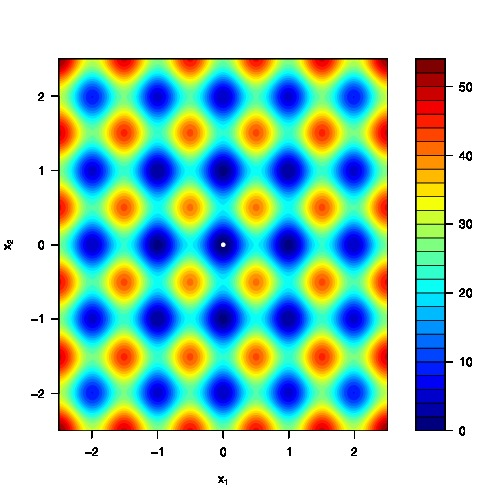
\includegraphics[width=0.49\textwidth]{./figures/rastContour.jpg}
	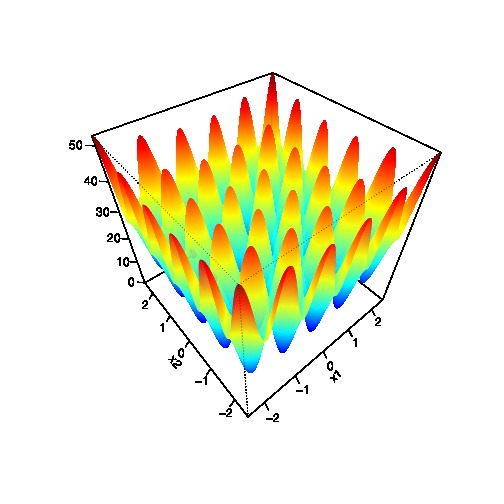
\includegraphics[width=0.49\textwidth]{./figures/rastPersp.jpg}
	\vspace{-0.5cm}
	\begin{eqnarray}
	f(x_1, x_2) &=& \sum_{i=1}^2\left[x_i^2-10\cos(2\pi x_i)\right] + 2(10)\\
	\label{rastEq}
	\text{Minimum}&:& f(0, 0)=0\nonumber
	\end{eqnarray}
	%\begin{eqnarray}
	%f(\bm{x}) &=& 10n+\sum_{i=1}^n\left[x_i-10\cos(2\pi x_i)\right]
	%\end{eqnarray}
	\end{figure}
	
	\vspace{-0.5cm}
	%
	The Rastrigin function \cite{rastCite} is a commonly used test function on genetic algorithms; in this setting it offers an interesting example for considering convergence for highly multimodal objective functions.
	% located  nadir  lowest point objective 
	The global behavior of Rastrigin is dominated by the spherical function, $\sum_i x_i^2$, however Rastrigin has been oscillated by the $\cos(.)$ function, and shifted, so that it achieves a global minimum value of 0 at the lowest point, of its lowest trough at (0, 0).
	
	% distributed so tightly 
	%Since the Rastrigin function has so many minima that are both close in magnitude and in location, Rastrigin  
	
% 	{\color{red}
% 	
% 	********* Below this point the document is incomplete... A work in progress... **********
% 	
% 	%
% 	%A GP surrogate mean model fit of the mean 
% 	\begin{wrapfigure}{l}{0.35\textwidth}
% 	\vspace{-1.5cm}
% 	\hspace{-1.3cm}
% 	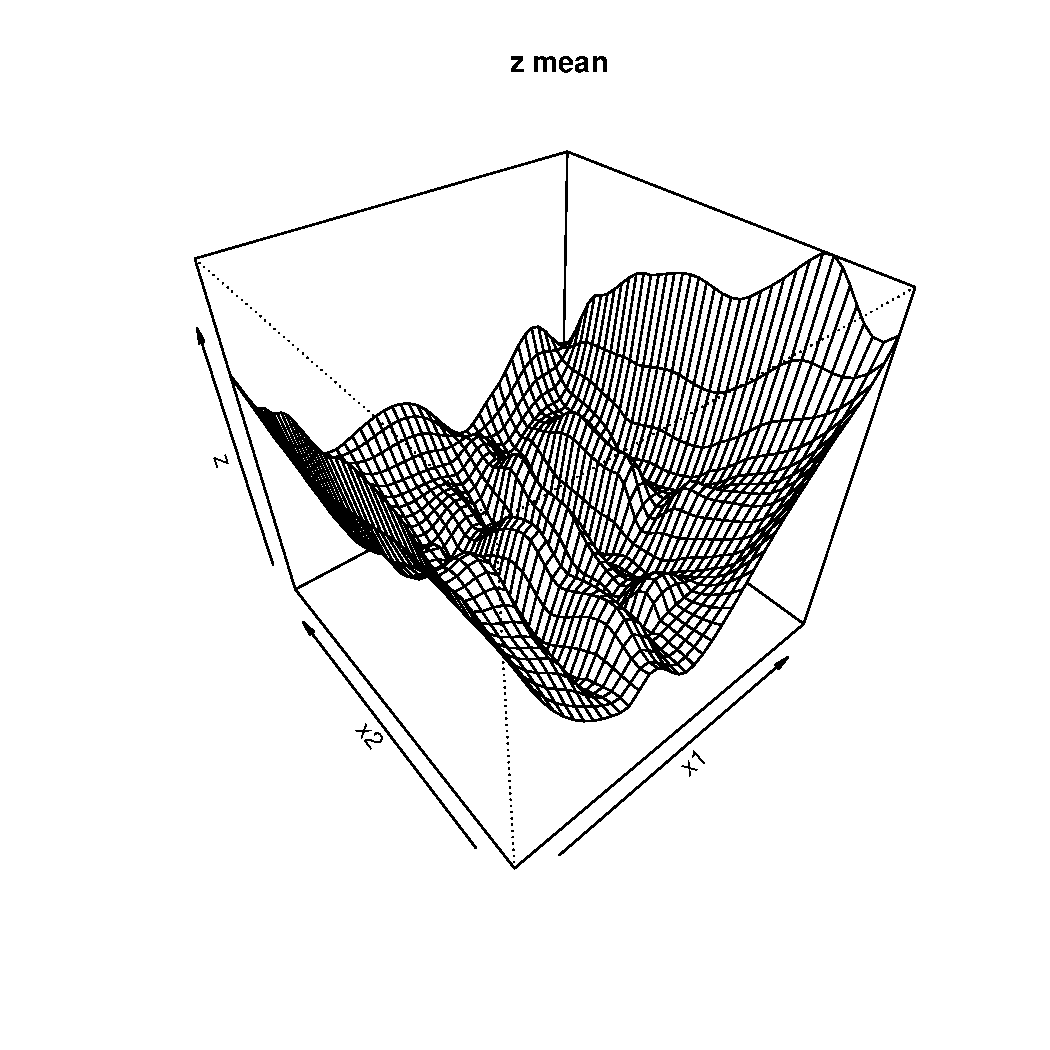
\includegraphics[width=0.4\textwidth]{./figures/gpMeanRastHard.pdf}
% 	\vspace{-2.cm}
% 	\caption{Rastrigin predictive mean surface after 90 iterations.} % of the surrogate modeling procedure. }
% 	\label{roseGP}
% 	\end{wrapfigure}
% 	%
% 	%
% 	%problem purely from a modeling perspective
% 	Rastrigin is a much more difficult modeling problem than Rosenbrock.
% 	%
% 	Purely from the perspective of optimization, it is not important to model the entire function well; it is only import to explore just broadly enough so as to gather enough data to model the minima well.
% 	%
% 	Rastrigin's many minima are both close in magnitude and in location, thus it would require a lot of data distributed all over the space to accurately model the entire function, but EI criteria specifically avoids large values of $f$ that would otherwise provide accurate predictive models as seen in Figure (\ref{roseGP}).
	%
	
	%
	Tuning $\lambda$ and $w$ in this case requires careful consideration of how Rastrigin's many modes effect the exploration process.
	%
	Again the basic parameter tuning strategy is to first determine an appropriate value for $\lambda$, then tune $w$ conditionally on the expected behavior of the EWMA statistic for the chosen value of $\lambda$.
	%
	Rastrigin's many modes mean that as the objective landscape is explored, the algorithm will regularly find features indicative of possible new minima. %  of the objective landscape proceeds 
	%
	Initially this drives up the value of the EI criterion, but as each of these modes are adequately explored, and disregarded, the EI value experiences large downward shifts.
	%
	To accurately track these large shifts it is required to choose a large value for $\lambda$. 
	%
	Recall that typical values for $\lambda$ lie in the range $0.1\le\lambda\le0.3$; in this case it is sufficient to simply choose the upper threshold of this typical range, thus $\lambda$ is set to $\lambda=0.3$.
	%
	Since the increased value for $\lambda$ results in a more actively fluctuating EWMA statistic, the choice of $w$ must reflect this knowledge.
	%
	In the default case $w=30$, but to account for the increased fluctuations brought about by a larger $\lambda$ value, $w$ is increased to $w=40$. 
	
	
	%upper and lower
	As before, the initial EWMA convergence chart, seen in Figure (\ref{rastEWMAStart}, {\it left}), indicates a lack of control, as demonstrated by the violations of the control limits inside the control window.
	% of Eq. (\ref{rastEq}).by right panel of
	This out-of-control chart indicates that the algorithm has not yet converged, which is confirmed Figure (\ref{rastEWMAStart}, {\it right}), showing that initially the smallest objective value
	%
	%
	\begin{wrapfigure}{l}{0.5\textwidth}
	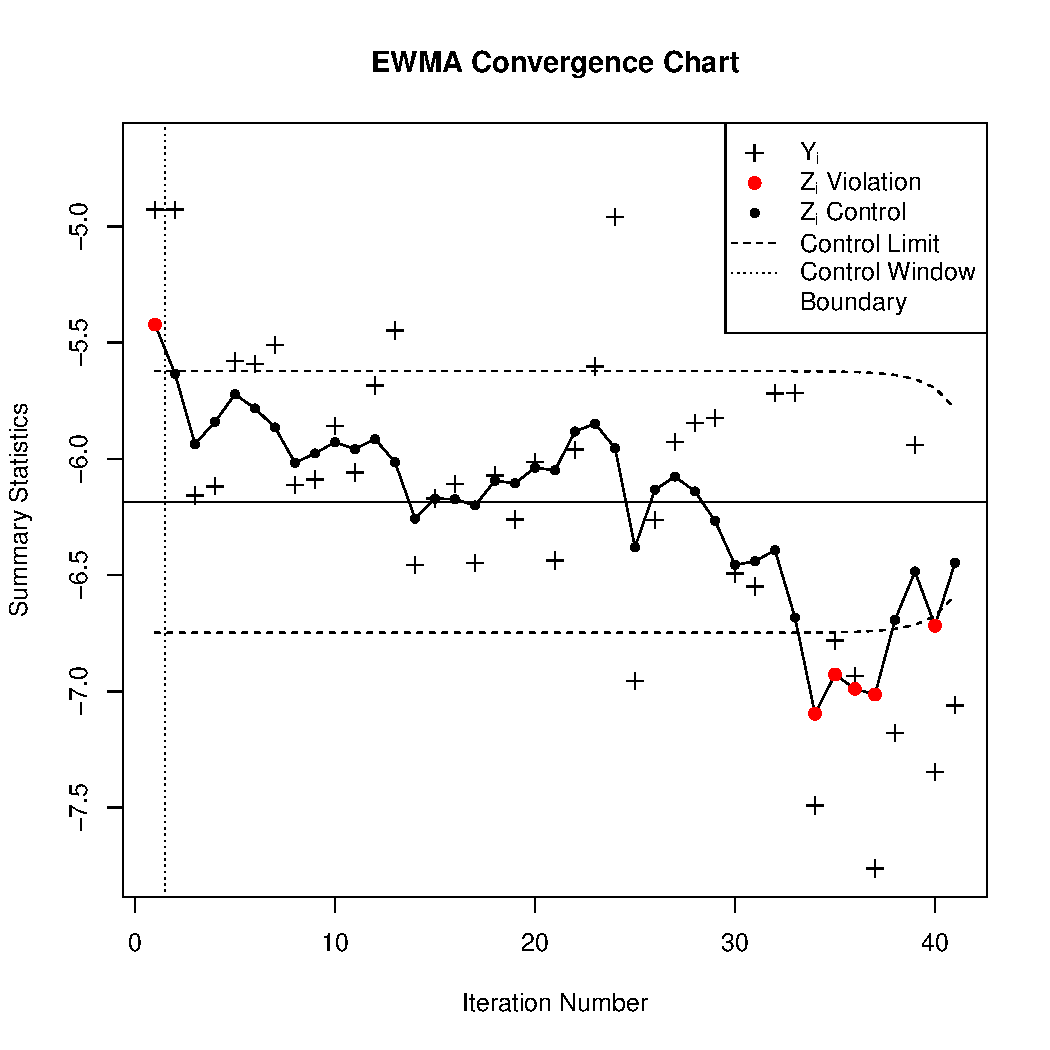
\includegraphics[width=0.245\textwidth]{./figures/ewmaConvChartRastHardStart.pdf}
	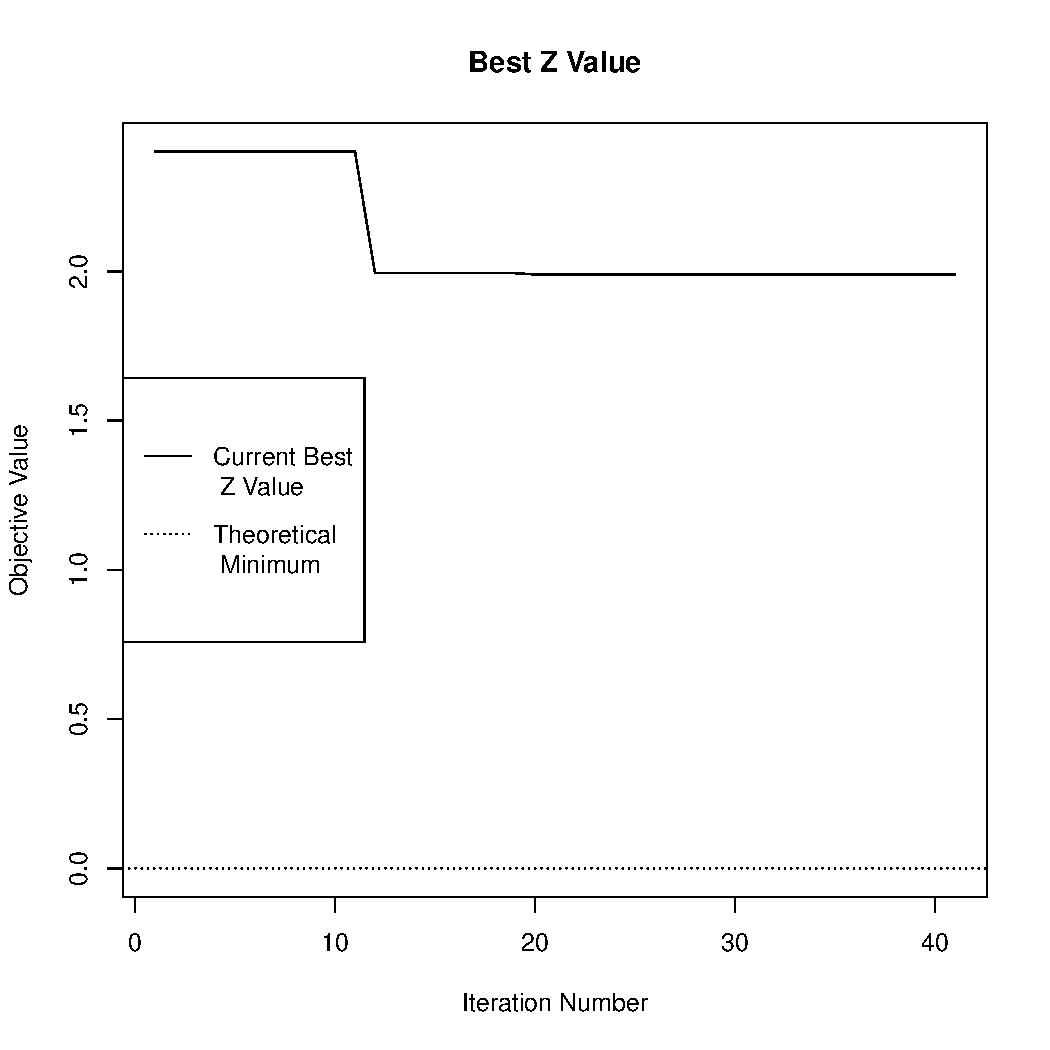
\includegraphics[width=0.245\textwidth]{./figures/bestZRastHardStart.pdf}
	\caption{Initial EWMA convergence chart and smallest objective function value. }
	\label{rastEWMAStart}
	$~$\\
	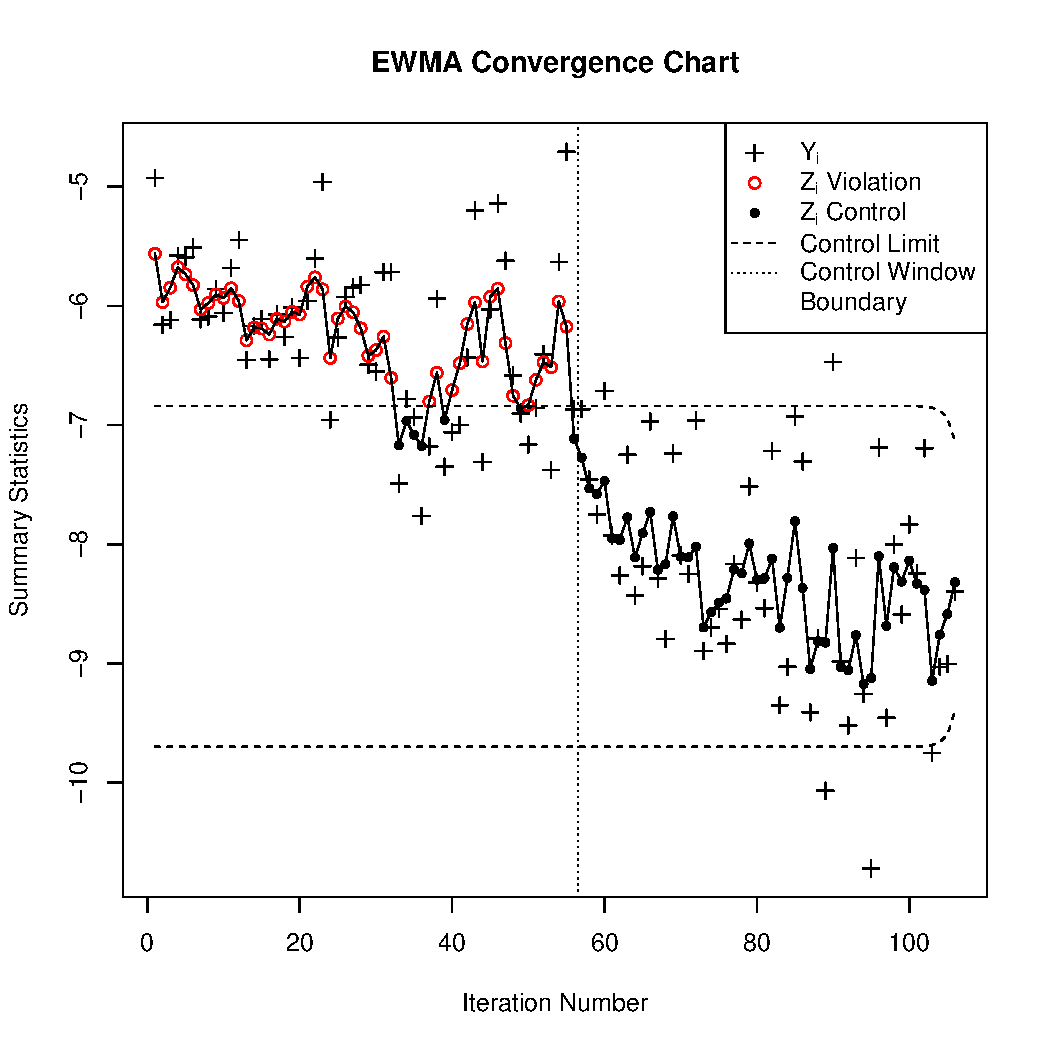
\includegraphics[width=0.245\textwidth]{./figures/ewmaConvChartRastHardEnd.pdf}
	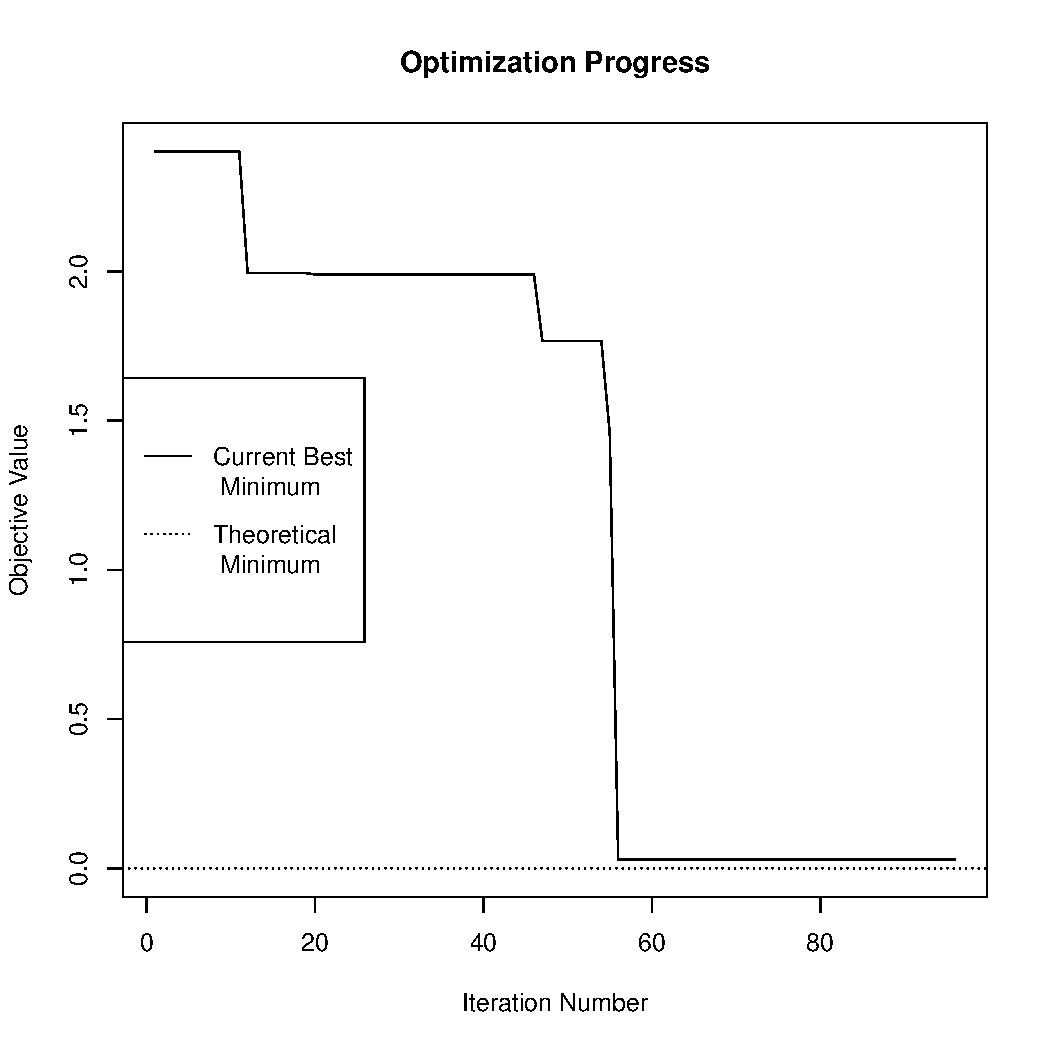
\includegraphics[width=0.245\textwidth]{./figures/bestZRastHardEnd.pdf}
	\caption{Final EWMA convergence chart and smallest objective function value. }
	\label{rastEWMAEnd}
	\end{wrapfigure}
	%
	%in the initial state
	is far from the theoretical minimum.
	%the right panel shows that 
	Considering Figure (\ref{rastEWMAEnd}, {\it right}), after about 55 iterations the algorithm finds nearly the theoretical minimum, but it takes until about iteration 90 for enough of the large EI values to move out of the control window so that the EWMA control chart can claim convergence.
	%
	Notice that since the value of $\lambda$ was increased here, the fluctuations in the EWMA statistic have also increased as compared with Figure (\ref{roseEWMAEnd}, {\it left}).
	%Smaller values of $w$ would open up here 
	The larger value of $w$ is needed to alleviate the possibility of introducing small sample biases, introduced by the increased EWMA fluctuations, in long-run average estimates in computing the control limits.
	%
	Thus decreasing $w$ here would increase the prevalence of false claims of convergence.
	
	\clearpage
	%
	%
	\subsection{Easom}
	%
	%
	
	%
	%
	\begin{figure}[!h]
	\centering
	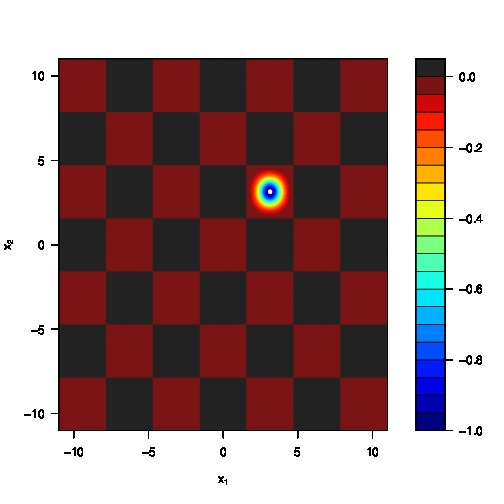
\includegraphics[width=0.49\textwidth]{../../figures/easomContour.jpg}
	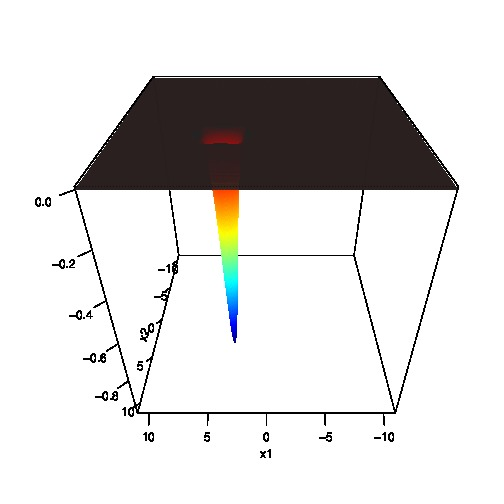
\includegraphics[width=0.49\textwidth]{../../figures/easomPersp.pdf}
	\vspace{-0.2cm}
	\begin{eqnarray}
	f(x,y) &=& -\cos \left(x_1\right)\cos \left(x_2\right) \exp\left\{-\left[\left(x_1-\pi\right)^{2} + \left(x_2-\pi\right)^{2}\right]\right\}\\
	\text{Minimum}&:& f(\pi, \pi)=-1\nonumber
	\end{eqnarray}
	\end{figure}
	\vspace{-0.3cm}
	
	%
	If the Rastrigin function is an extreme example of how convergence looks in multimodal situations, then the Easom function is on the polar opposite end of that modality scale.
	%Further inspection of the exponential; (fundamentally they are both trigonometric in nature) in nature; (fundamentally both minima are trigonometric)
	Easom's single substantial minimum is similarly as sharp as the minima of Rastrigin (fundamentally they are both trigonometric in nature), however Easom's oscillations have been scaled by the exponential function so as to only emphasize the single mode present at $(\pi, \pi)$, at which, the objective value is allowed to reach its global minimum of $-1$.
	%, for all practical reasons,
	As $x$ values deviate from $\pi$, the exponential term quickly becomes vanishingly small, and thus the remainder of the search region lies practically at 0. 
	
	%
	%
	
	%
	Again to tune $\lambda$ and $w$ I consider how the EI may react to features (or lack there of in this case) of the objective function. % a search region that is so devoid of substantial features.
	%indicative of new minima
	Since Easom is so devoid of features, the objective search may only seldomly visit the single mode.
	% primary understand thus required to
	Furthermore, since the primary mode is relatively compact, it should only require a few observations from this mode to gather its general shape and minimum value.   
	%
	Thus, EI values should remain relatively consistent through out the search; the EI value only shifts slightly as the mode is quickly understood and the remainder of the unseen search space is eventually filled in.
	%the expectation is that 
	Since the EI will only experience slight shifts, this naturally implies a small value for $\lambda$.
	% for $\lambda$s
	Choosing $\lambda$ to be the lower limit from the typical range, $\lambda=0.1$, yields a lot of smoothing in the EWMA statistic.
	%%with a similarly sharp lone minimum among an otherwise flat surface.
	This heavily smoothed EWMA statistic enables the EWMA convergence chart to notice very small shifts in the underling $\E{\log\ix}$ value. 
	%to subject the
	The small value chosen for $\lambda$ implies small fluctuations in the EWMA statistic, and thus there is less opportunity to introduce small sample biases in the long run average estimates. 
	% 
	A relatively small control window is thus desirable in this case since it provides a more recent picture of the state of control, without experiencing much bias from large fluctuations.
	%in this case
	In this case $w$ was chosen to be $w=20$ iterations long.
	
	%that; seen in the previous examples the initial charts On the one hand, t
	The previously seen initial EWMA convergence charts, Figures (\ref{roseEWMAStart}) and (\ref{rastEWMAStart}),
	%
	%
	\begin{wrapfigure}{l}{0.5\textwidth}
	\includegraphics[width=0.245\textwidth]{../../figures/ewmaConvChartEasomMedStart.pdf}
	\includegraphics[width=0.245\textwidth]{../../figures/bestZEasomMedStart.pdf}
	\caption{Initial EWMA convergence chart and smallest objective function value. }
	\label{easomEWMAStart}
	$~$\\
	\includegraphics[width=0.245\textwidth]{../../figures/ewmaConvChartEasomMedEnd.pdf}
	\includegraphics[width=0.245\textwidth]{../../figures/bestZEasomMedEnd.pdf}
	\caption{Final EWMA convergence chart and smallest objective function value. }
	\label{easomEWMAEnd}
	\end{wrapfigure}
	%
	%
	%
	demonstrate a
	lack of convergence through a continually decreasing EWMA statistic which violates the control limits inside the control window.
	%the lack of{\it no}falling; out-of-control points  beyond the control window  (see Figure (\ref{easomEWMAStart})
	In contrast, this example experiences much more subtle EI shifts, and thus, the initial pre-converged state, seen in Figure (\ref{easomEWMAStart}), is indicated by the lack of any control limit violations.
	% thus far
	This comes from the fact that initially the objective search has not resulted in a substantial indication that the EI value has decreased enough to signal convergence.
	%%initial EWMA statistics violate the control limits beyond the control window.
	As the search continues, the lone minimum is eventually found, and the EWMA convergence chart realizes convergence as the control region shifts downward and the control limits shrink. 
	
	
% 	\begin{itemize}
% 	\item[\checkmark] Describe function \cite{easomCite} 
% 	\item[\checkmark] write function down
% 	\item[\checkmark] Pictured interval.
% 	\item describe strategy for identifying convergence relative to characteristics of function (or expected characteristics of function).
% 	\item thus choose $\lambda$ and $w$ appropriately.
% 	\item discuss convergence behavior (save)
% 	\item
% 	\item Easom is very flat function
% 	\item adjust lambda to, $\lambda=0.1$ to compensate.
% 	\item adjust window size $w=20$ to pick up smaller changes inherent to smaller lambda.
% 	\end{itemize}
	
	\clearpage
	%
	%
	\subsection{Lockwood Pump-And-Treat Case Study}
	%
	%
	
	%closed form
	The previous examples have focused on analytical functions with known minima.
	%
	This is done for the sake of developing an intuition for tuning the EWMA convergence chart parameters.
	%
	However, in most practical optimization problems it is not possible to visualize to objective function so straight forwardly, or derive theoretical minima in this way.
	%
	Thus, to demonstrate the use of the EWMA convergence chart in one such practical situation, I consider the Lockwood pump-and-treat problem presented by Matott et al. \cite{lockCite}. \\
	
	%
	%
	\begin{wrapfigure}{l}{0.5\textwidth}
	\vspace{0.3cm}
	\centering
	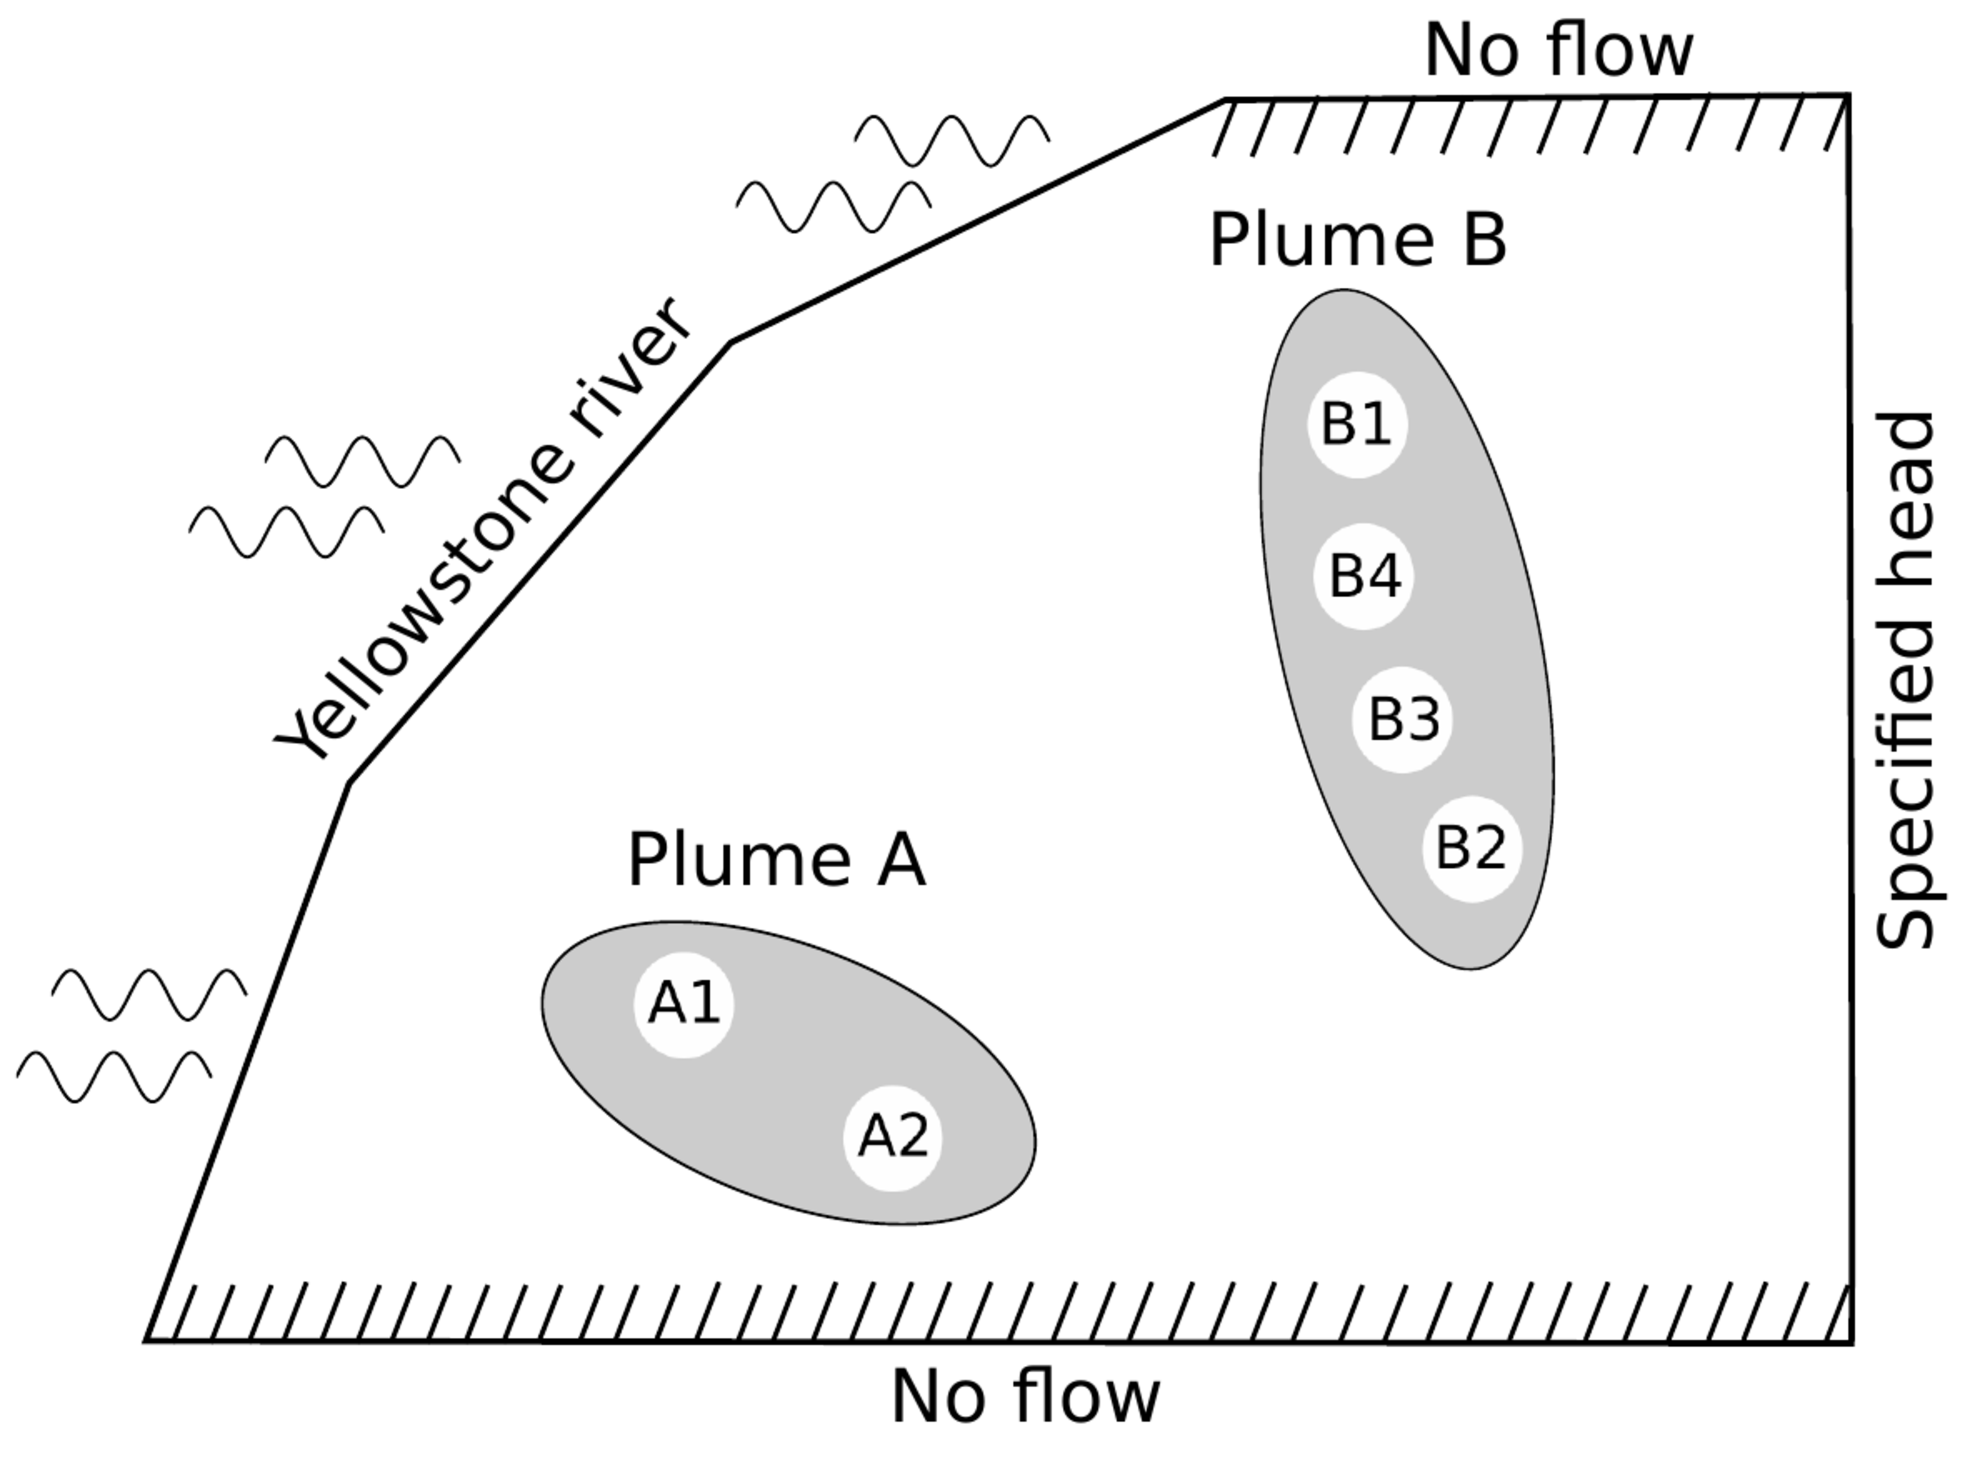
\includegraphics[width=0.5\textwidth]{./figures/Lockwood_Site_Simple.pdf}
	\caption{The Lockwood pumping site}
	\label{lockSite}
	\end{wrapfigure}
	\vspace{-0.3cm}
	%
	%
	
	%
	The Lockwood pump-and-treat case study considers a pumping site for chlorinated solvents located north-east of Billings, Montana, along the Yellowstone River.
	%
	The site, seen in Figure (\ref{lockSite}), contains two plumes for pumping, Plume A and Plume B, containing two and four wells respectively.
	%
	The objective is to determine the lowest cost pumping rates for each of these six wells such that contamination from the plumes does not reach the Yellowstone River.
	
	%
	%
	
	%, to ensure that an optimal solution never relies upon regular river contamination.a function proportional to 
	Thus the objective function, $f(\bm{x})$, can be expressed as the sum of the inputs, with penalties associated with contamination of the river. % by each plume, $c_A(\bm{x})$, $c_B(\bm{x})$. %$c_A(\bm{x})$ and $c_B(\bm{x})$ indicating that the  
	%, is the cost of operating the pumps, in USD; additionally, $f$ heavily penalizes solutions that contaminate the river.
	\begin{equation}
	f(\bm{x}) = \sum_{i=1}^6 x_i +  2\big[ c_A(\bm{x}) + c_B(\bm{x}) \big] + 20000 \big[ \oner_{c_A(\bm{x})>0} + \oner_{c_B(\bm{x})>0} \big] 
	\end{equation}
	%with simple search boundaries, \mbox{$0\le x_i\le20,000$} set for each pumping rate.
	Here $c_A(\bm{x})$ and $c_B(\bm{x})$ indicate the amount of contamination of the river by each plume, and $\bm{x}$ represents the pumping rate, $Q_i$, for each of the six wells.
	%, \mbox{$\left[x_1, ..., ~x_6\right] = \left[Q_{A1}, ~Q_{A2}, ~Q_{B1}, ~Q_{B2}, ~Q_{B3}, ~Q_{B4}\right]$}.
	Each $x_i$ is bounded on the relatively large interval, \mbox{$0\le x_i\le20,000$}. 
	%
	The full problem, considering all six wells, defines a six-dimensional optimization problem, but for the sake of better understanding the dynamics of the problem, it is instructive to first consider the simplified single plume problem. 
	%to understand the behavior of the EI criterion I first consider simplified into%with respect to $f$;
	The two-dimensional problem provides a nice setting for understanding the a simplified version of EI behavior, and furthermore the simplified setting develops an expectation for the EI behavior in the full \mbox{six-dimensional problem.}
	
% 	\clearpage
	%
	%
	\subsubsection{Two-Dimensional Single Plume Problem}
	%
	%
	
	%
	%surrogate model of the surrogate modeling procedure.
	\begin{wrapfigure}{l}{0.5\textwidth}
	\vspace{-1.1cm}
	\hspace{-1cm}
	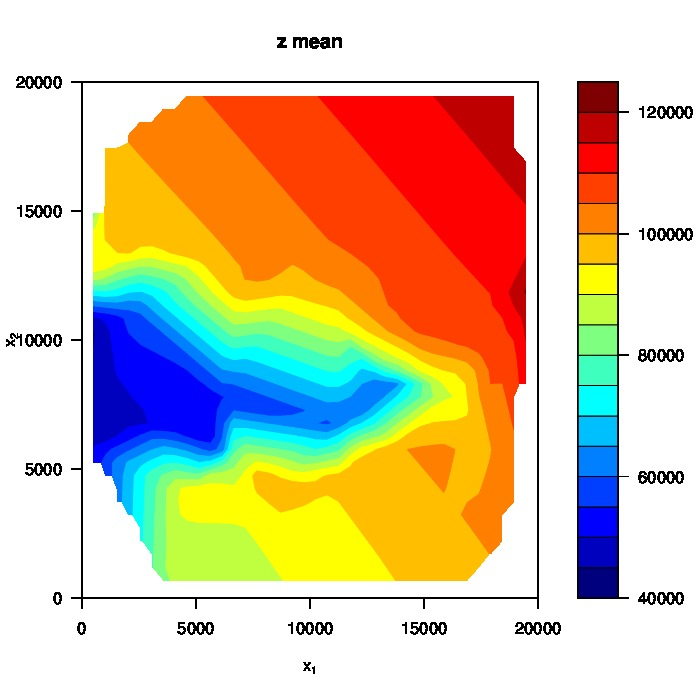
\includegraphics[width=0.5\textwidth]{./figures/gpMeanLock240000.jpg}
	\vspace{-0.9cm}
	\caption{The GP mean predictive loss surface for the two well Lockwood problem. }
	\label{lockGP}
	\end{wrapfigure}
	%
	%
	
	%and all of the wells associated
	The simplified search only focuses on the two wells of Plume A, and all other wells associated with Plume B, are fixed in the center of the search domain at 10,000. 
	% we are allowed to visualize the search space through the use of the GP surrogate model.
	By limiting the problem in this way, it allows for visualization of the search space via the GP surrogate model.
	%
% 	In Figure (\ref{lockGP}) the GP predictive surface is seen after 400 observations of $f$.
	%demonstrates
	Figure (\ref{lockGP}) shows that much of the search space is dominated by relatively flat and consistent high loss (i.e. hot/warm colors), resulting from contamination penalties.
	%
	However, for low rates in $x_1$ and intermediate rates in $x_2$ there is a rough fissure of low cost values.
	%
% 	This fissure of relatively low loss is associated with low, to intermediate, rates in $x_1$ and intermediate rates in $x_2$. 
	%
	Due to the magnitude of the contamination penalties, the walls of the Fosse seen in Figure (\ref{lockGP}) are very steep.
	%
	Furthermore, the features of the fissure floor are fairly detailed, and easy to overlook especially when compared to the relatively large search space (i.e. \mbox{$0\le x_i\le20,000$}).
	
	\clearpage
	%
	%
	
	%
	Thus for determining convergence in this setting, I consider this problem to be similar to, and somewhere between, the Rosenbrock ($\lambda=0.2$) and Rastrigin ($\lambda=0.3$) test situations.
	%
	Thus $\lambda=0.25$ is an appropriate choice for the smoothing parameter.
	%% 	Since, $\lambda$ is in the upper region of the typical $\lambda$ range a large value for $w$ is appropriate.
	Again I consider the value of $\lambda$ to inform the choice of $w$.
	%
	Since $\lambda$ is in the upper region of the typical $\lambda$ range, a large value for $w$ is appropriate.
	%search space is  it is worth additional  not possible to get 
	Furthermore, since the search space is so large, the choice of a conservatively large $w$ is recommended.
	% 
	In this application $w=50$ has shown to be effective. 
	

% 	\clearpage
	%
	%
	\begin{wrapfigure}{l}{0.5\textwidth}
	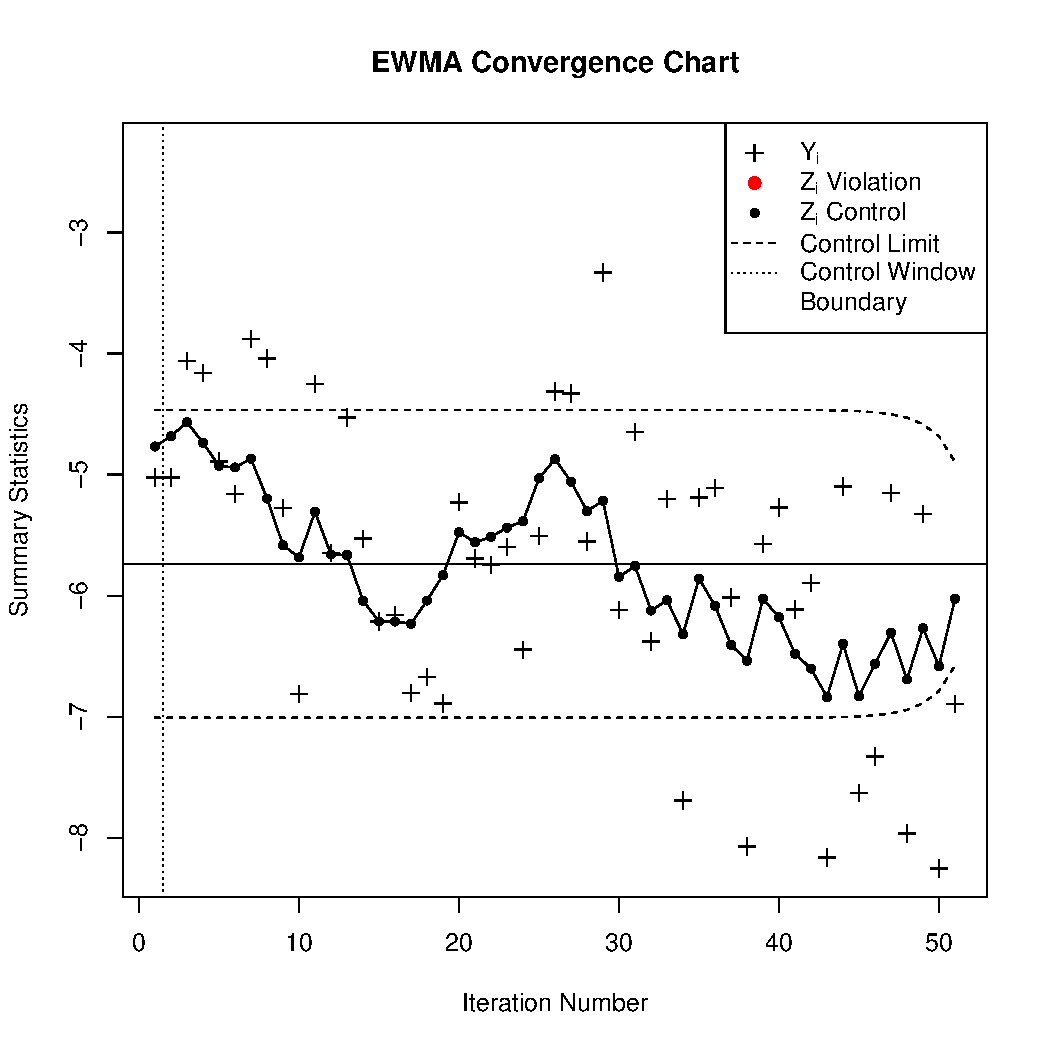
\includegraphics[width=0.245\textwidth]{./figures/ewmaConvChartLock240000Start.pdf}
	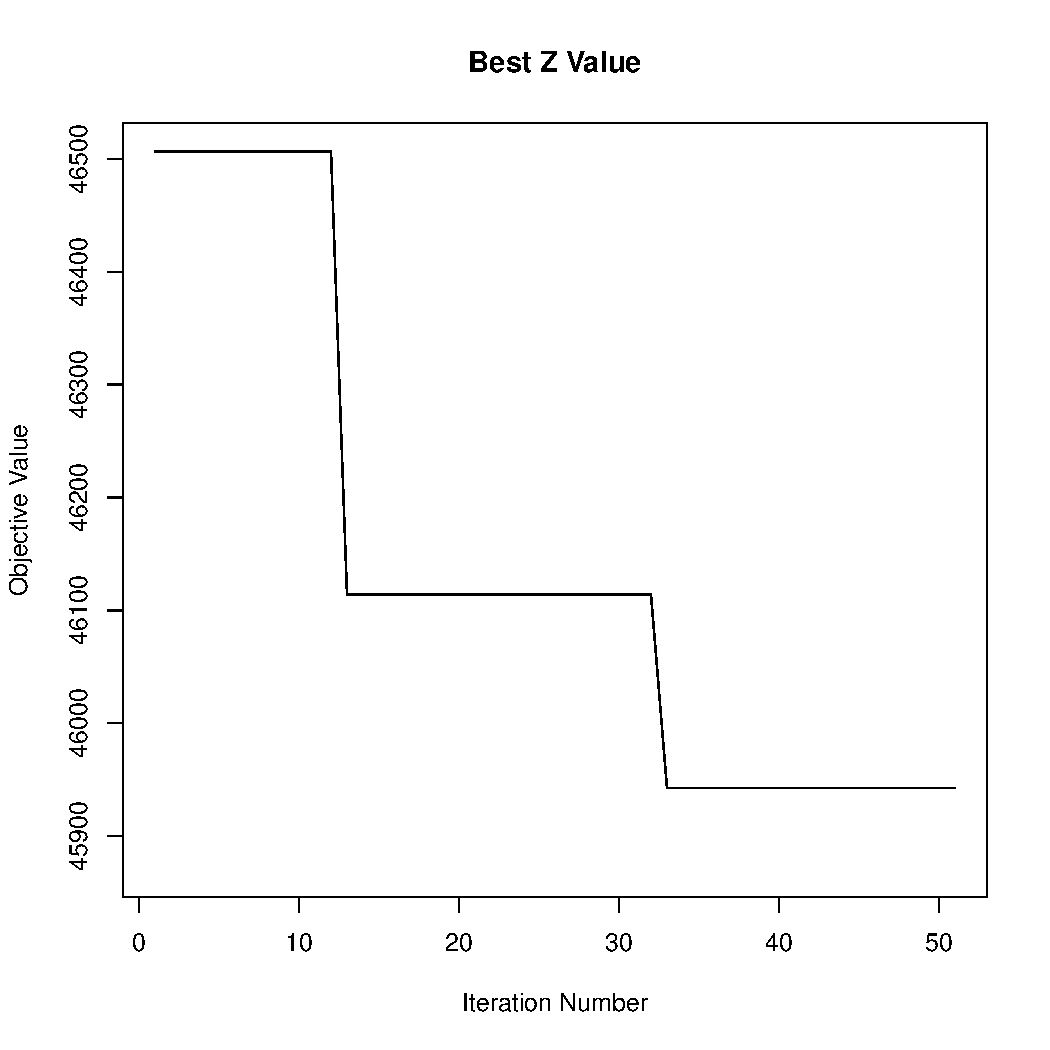
\includegraphics[width=0.245\textwidth]{./figures/bestZLock240000Start.pdf}
	\caption{Initial EWMA convergence chart and smallest objective function value. }
	\label{lock2EWMAStart}
	$~$\\\\
	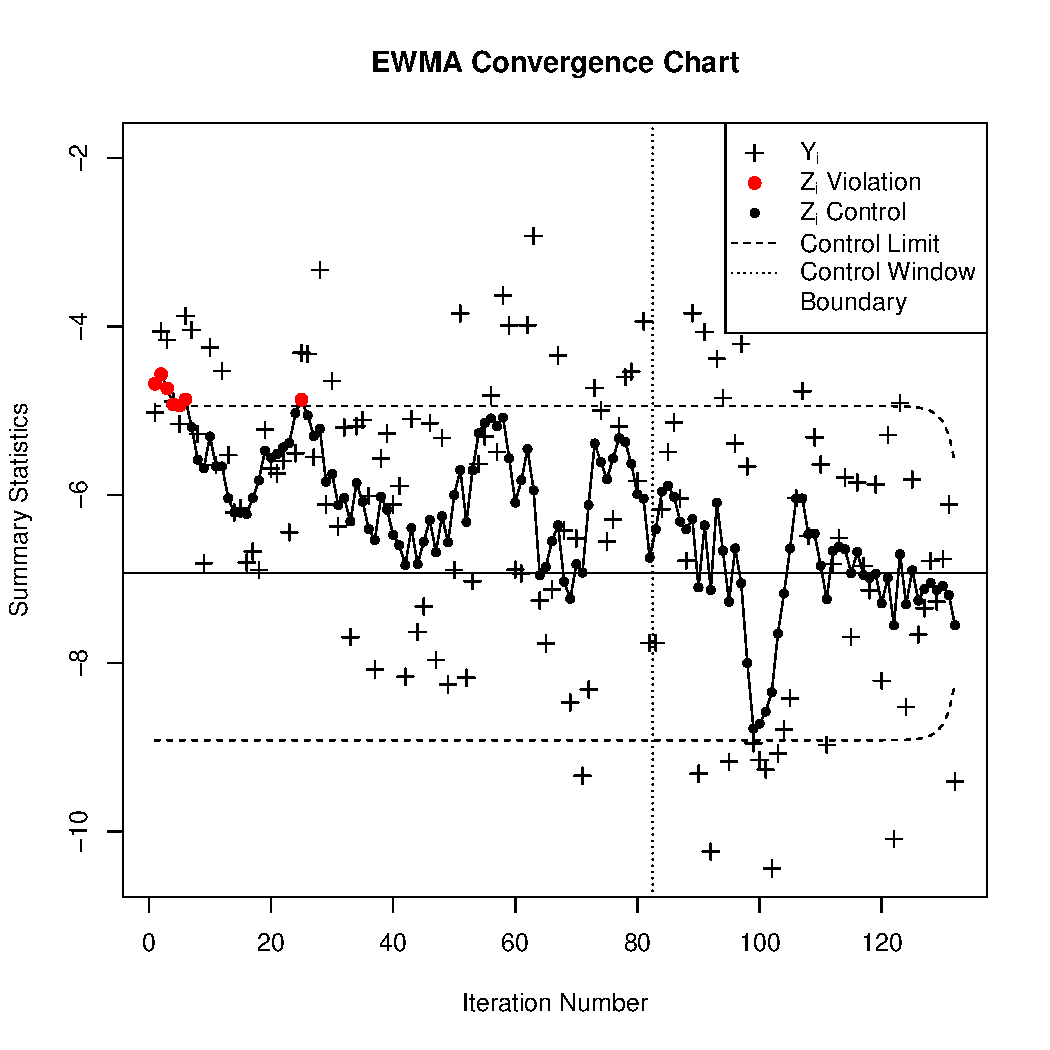
\includegraphics[width=0.245\textwidth]{./figures/ewmaConvChartLock240000End.pdf}
	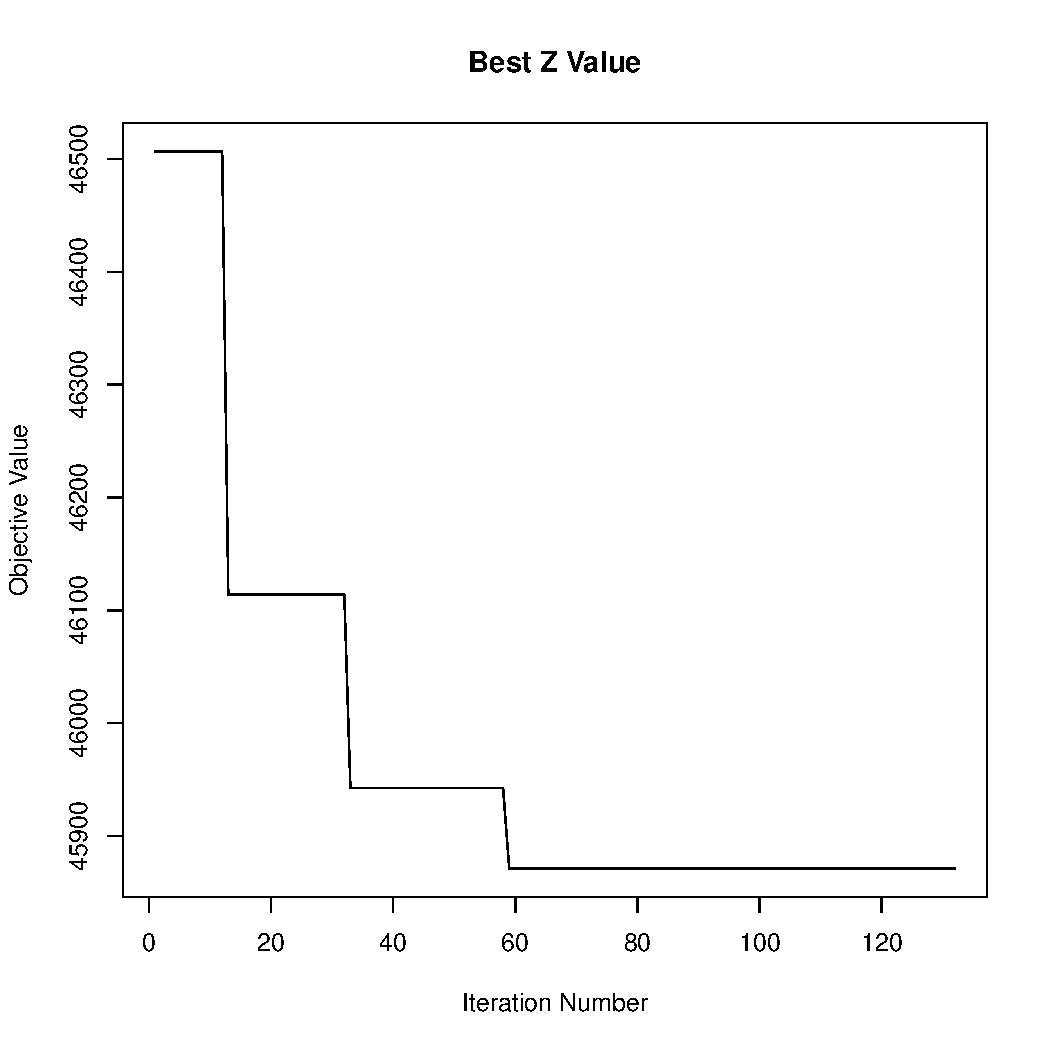
\includegraphics[width=0.245\textwidth]{./figures/bestZLock240000End.pdf}
	\caption{Final EWMA convergence chart and smallest objective function value. }
	\label{lock2EWMAEnd}
	\end{wrapfigure}
	%
	%
	
	%
	Initially the convergence chart, seen in \mbox{Figure (\ref{lock2EWMAStart}, {\it left}),} does not show any violations of the control limits.
	%improvement in the context of a state of
	Thus, \mbox{Figure (\ref{lock2EWMAStart})} does not show any signs of movement from the initial state of pre-convergence and indicates that more iterations are need to achieve convergence. 
	%as converged, 
	After about 130 iterations of optimization, violations of the upper control limit arise, indicating that the routine has explored the space \mbox{sufficiently} to announce convergence, as seen in \mbox{Figure (\ref{lock2EWMAEnd}, {\it left}).}
	%
	
	%
	%
	
	%
	Further analysis of the smallest observed objective values, in each of these figures, indicates that indeed this search has converged to pumping rates that are consistent with those originally reported by Matott et al. \cite{lockCite}. 
	%
	Here the smallest objective value is given for \mbox{$\bm{x} \approx \left[13,~5857,~10000,...,~10000\right]$.}    
	
% 	$~$
	\clearpage
% 	\vspace{-0.5cm}
	%
	%
	\subsubsection{Full Six-Dimensional Problem}
	%
	%
	
	% as well
	The full optimization problem not only considers the two wells of Plume A, but additionally optimizes over the four wells in Plume B.
	%ality
	By increasing the dimension of the domain, this exponentially increases the space to be explored in the objective search.
	%
% 	For example, if each dimension of the domain is discretized to the integers on the set \mbox{$0\le x_i\le20,000$}, then increasing the dimension of the problem from two to six results in a $20,001^{(6-2)}\approx1.6\times10^{17}$ times larger space to search in the six dimensional problem.
	%is fantastically; this space is naively explored and thus
	Despite the large increase in the space of the objective search, recall that much of this space can be confidently ignored after the initial collection of $\bm{X}$.

% 	\clearpage
	%
	%
	\begin{wrapfigure}{l}{0.5\textwidth}
	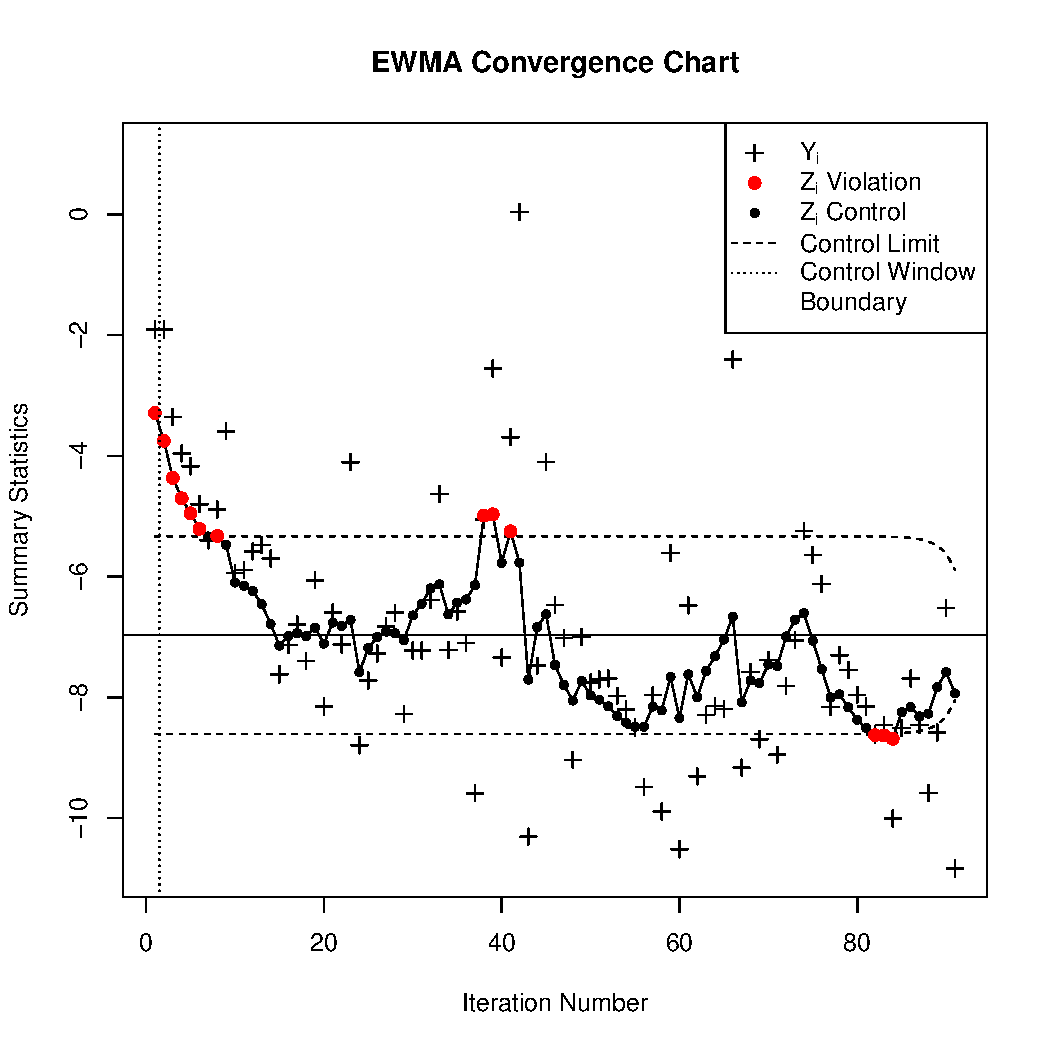
\includegraphics[width=0.245\textwidth]{./figures/ewmaConvChartLock6Three20000Start.pdf}
	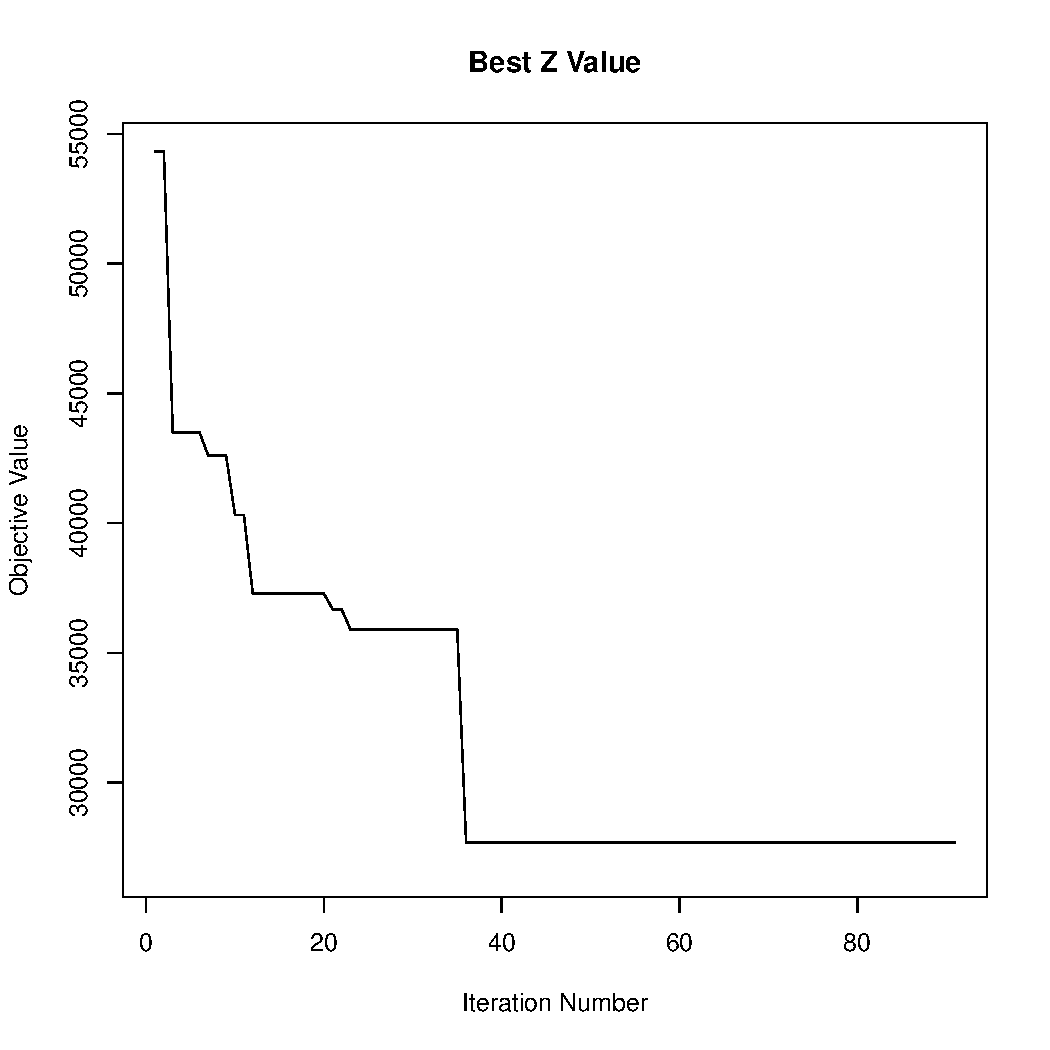
\includegraphics[width=0.245\textwidth]{./figures/bestZLock6Three20000Start.pdf}
	\caption{Initial EWMA convergence chart and smallest objective function value. }
	\label{lock6EWMAStart}
	$~$\\
	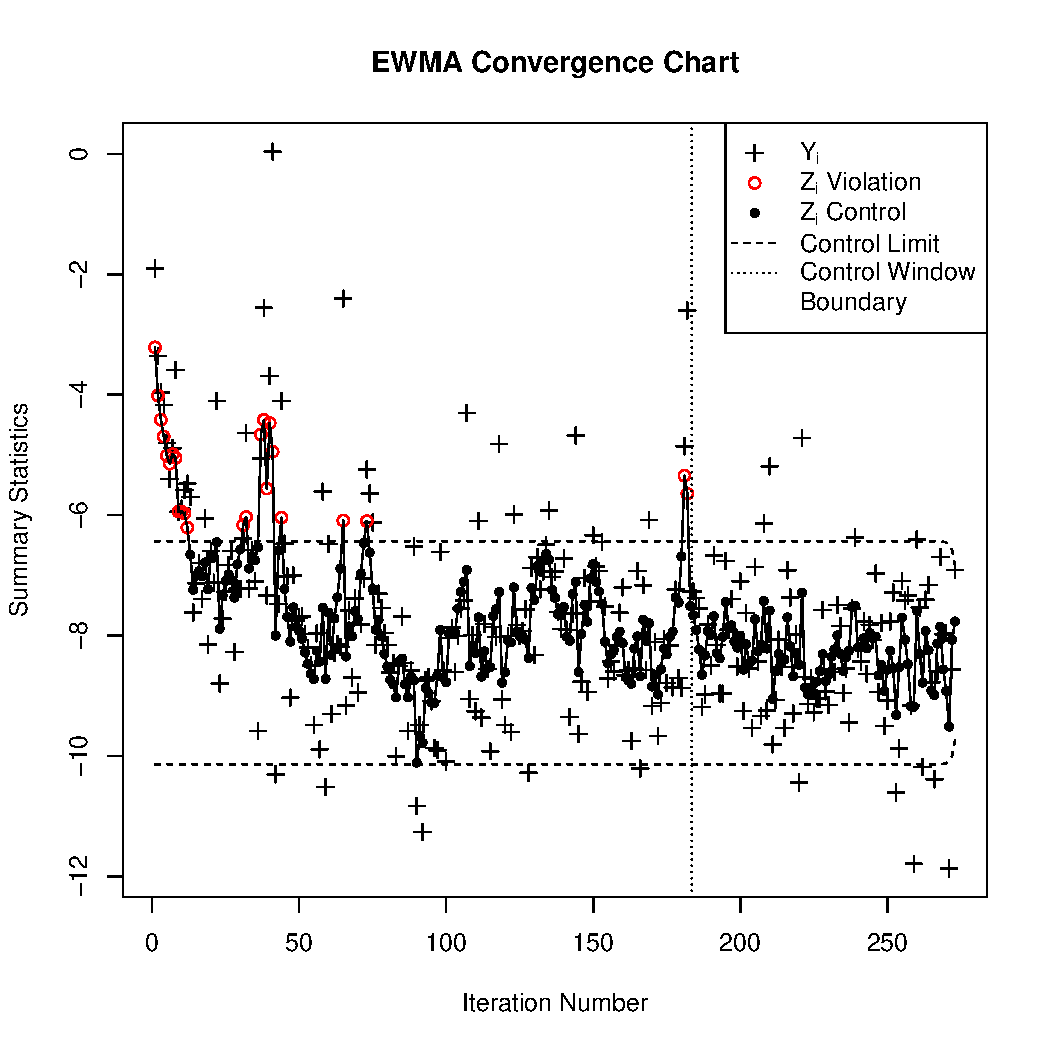
\includegraphics[width=0.245\textwidth]{./figures/ewmaConvChartLock6Three20000End.pdf}
	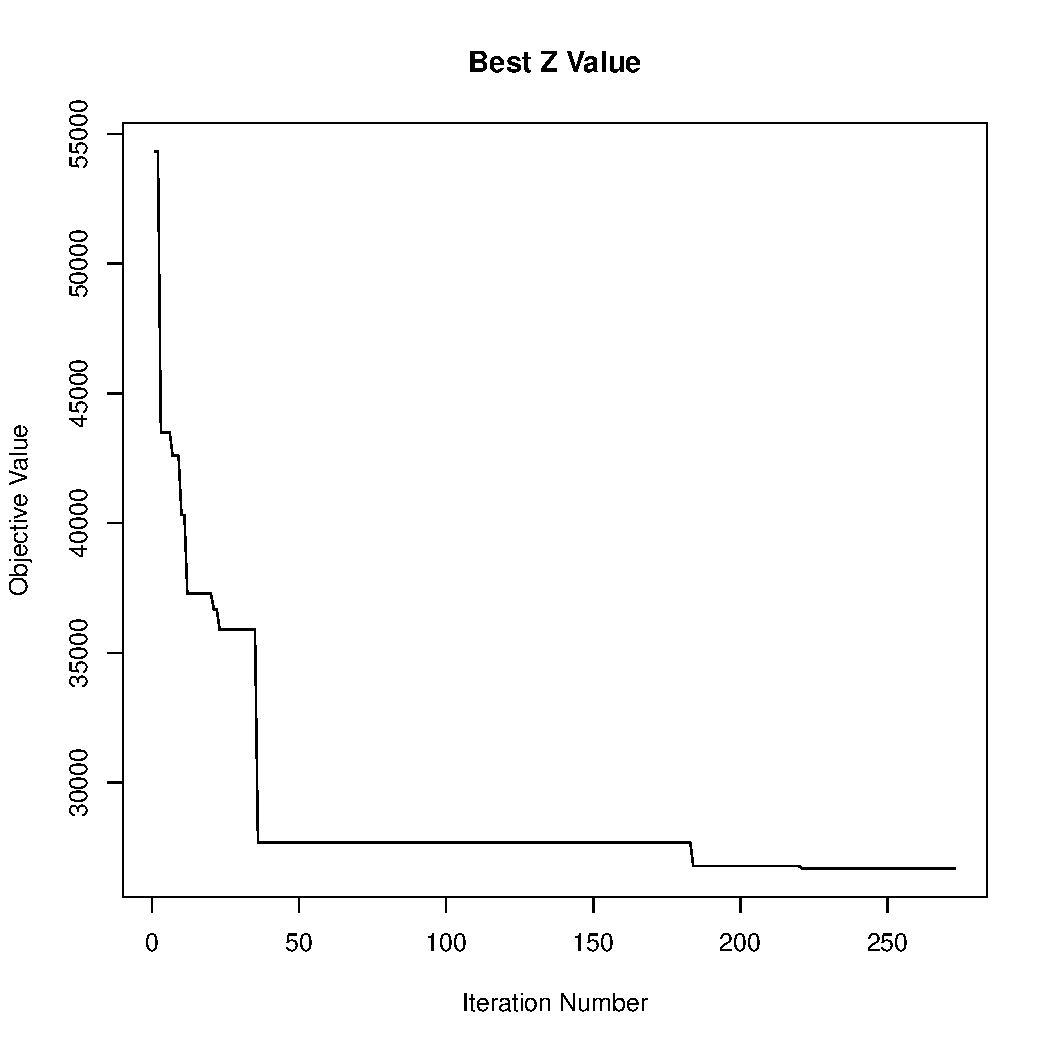
\includegraphics[width=0.245\textwidth]{./figures/bestZLock6Three20000End.pdf}
	\caption{Final EWMA convergence chart and smallest objective function value. }
	\label{lock6EWMAEnd}
	\end{wrapfigure}
	%
	%
	
	
	% #that I should expect
	Aside from the vastly larger domain to be searched, there is no information indicating substantially different behavior from the addition of Plume B.
	%
	Thus considering the behavior of the two dimensional problem, it is reasonable to assume similar values for $\lambda$ and $w$.
	%I keep
	Here the value of $\lambda$ is kept the same as the two dimensional problem at $\lambda=0.25$, thus reflecting an intermediately lumpy objective function.
	%I increase the size of the control window to $w=60$.
	However to be conservative, considering the increased size of the domain, the size of the control window is increases to $w=90$. 
	
	%Figures (\ref{lock6EWMAStart}) and (\ref{lock6EWMAEnd})EWMA convergence
	Again considering the initial and final EWMA convergence chart, we see that initially in Figure (\ref{lock6EWMAStart}, {\it left}) the chart does not indicate convergence.
	%the right indeed best Z value
	%Considering the smallest objective values observed, Figure (\ref{lock6EWMAStart}, {\it right}) indicates that indeed the objective search has not discovered a substantial minimum of $f$.
	%Considering Figure (\ref{lock6EWMAEnd}), we observe that a %This solution % the right panel of  we see that 
	%In Figure (\ref{lock6EWMAEnd}, {\it right}) after about 210 iterations, the algorithm finds its lowest cost solution to be seen in 500 iterations, corresponding to an \mbox{$\bm{x} \approx \left[433,~5911,~12290,~5353,~1782,~3177\right]$}.
	In \mbox{Figure (\ref{lock6EWMAEnd}, {\it right})} after about 210 iterations, the algorithm finds its lowest cost solution to be seen in 500 iterations, corresponding to \mbox{$f(\bm{x})\approx26696$} at \mbox{$\bm{x} \approx \left[0,~6195,~12988,~3160,~1190,~3163\right]$}.
	%
% 	This turns out to provide the lowest objective value to be discovered in 500 iterations of the algorithm.
	%we see
	Considering Figure (\ref{lock6EWMAEnd}, {\it left}), the EWMA convergence chart identifies this convergence after only about 270 iterations.
	%2.016075e-01 6.195005e+03 1.298804e+04 3.160273e+03 1.189587e+03 3.163334e+03
	%432.885  5910.821 12289.646  5352.652  1782.080  3177.451
% 	\mbox{$\bm{x} \approx \left[3,~7093,~13791,~4471,~6158,~111\right]$} $f(\bm{x}) \approx 31627$  
% 	

	
\clearpage
\doublespacing
% 	
% 	
\section{Conclusion}
% 	
% 	

%
% Identifying convergence in numerical optimization can be difficult due to the subjective nature of convergence. 
%
Through the use of SPC ideas the EWMA convergence chart provides an objective definition of convergence. % to give convergence a more objective definition.
%in this papeheredemonstrates its ability to
If properly tuned, the examples provided demonstrate how the  EWMA convergence chart may accurately, and efficiently, identify convergence in the context of GP surrogate model optimization.

%
%

%in optimization It is worth mentioning here that a
As for any optimization algorithm, the solution found may only be considered as good as the algorithms specific characterization of $f$.
%
Thus a poorly tuned surrogate modeling strategy may never optimize $f$ to its fullest extent.
%
In cases of poorly tuned optimization algorithms, the EWMA convergence chart presented here may only identify convergence with respect to the quality of the particular surrogate modeling strategy used.
%discovery 
Thus for poorly tuned surrogate modeling strategies the EWMA convergence chart may only identify that the algorithm has reached a point of diminishing returns; for correctly tuned surrogate modeling strategies this point corresponds with the realization of an optimal solution.
%at which the EWMA convergence chart claims convergence corresponds with the discovery of an optimal solution.
%
In either poor or correct tuning, the EWMA convergence chart identifies the moment at which it is beneficial to stop the routine to reflect upon the results.
%
%That is to say that when the either way stopping optimization  is useful to re-tune the algorithm, or enjoy the spoils of a succfull optimization algorithm.  

%
%

% all of the tested applications.
%provided my study with an effective outcome in all of the applications shown here 
%I have outlined a strategy that has shown to be effective, in my applications, for tuning the parameters of the EWMA convergence chart.
The strategy shown here for tuning $\lambda$ and $w$ demonstrates an empirically effective approach for tuning the EWMA convergence chart parameters. 
%
This approach is mainly useful due to its simplicity, although other more pointed methods may surely calculate more effective values.
%
Box et al. \cite{boxBook} demonstrates quantitative methods for choosing $\hat\lambda$ so as to minimize the sum of squared deviation of forcasting errors ($S_\lambda$), however this method was not considered here because it introduces additional optimization problems (albeit univariate and apparently simple).
%
The methods proposed by Box et al. may be extended to the EWMA convergence chart by considering some initial set of optimization iterations and considering the following bivariate optimization problem \mbox{$\left\{\hat\lambda, \hat w \right\} = \argmin_{\lambda, w} S(\lambda, w)$.} 

\clearpage
%
%

%, observed in the first few iterations of the algorithm,
The heuristics of the EWMA convergence chart were specifically chosen based on the behavior of EI criterion, however occasionally the initial optimistically high values of the EI criterion can produce situations that are susceptible to false convergence.
%
Since the first few iterations will always produce the first EI values to exit the control window, if these values are very large they may not be adequately tamed by the exponentially decreasing weights, as intended. % weights on these values may fail to taim this optimism.
%
Thus a conservative strategy for \mbox{combating} this initial optimism could involve removing the first few iterations of optimization from the analysis of the EWMA convergence chart.
%
This removal may be justified based on the notion that these observations are outliers that do not represent the initial pre-convergence state of control that is implicitly assumed here. 



%the  quantitative methods for estimating an optimal $\hat\lambda$, however this estimation introduces additional optimization problems (albeit univariate and apparently simple) and was not the focus of this work. % all be it univariate, optimization problem 
%

% , additionally Box et al. explains how to estimate specific a $\hat\lambda$ value tailored for each particular data set.
% 
% that has  in several cases although 

\clearpage
\newgeometry{ margin=1in, top=0.6in, footskip=0.4in }
\singlespacing
\bibliographystyle{plain}
\bibliography{./bibTex/msCite}
% \singlespacing
% \begin{thebibliography}{2}
% \bibitem{taddyOpt} M. Taddy, H. K. Lee, G. A. Grey, \& J. D. Griffin. (2008). {\em Bayesian Guided Pattern Search for Robust Local Optimization}. Technometrics, 51(4), 389-401.
% \bibitem{gpJasa} R. B. Gramacy, \& H. K. Lee. (2008). {\em Bayesian treed Gaussian process models with an application to computer modeling}. Journal of the American Statistical Association, 103, 1119-1130.
% \bibitem{tgp} R. B. Gramacy, (2007). {\em tgp: An R Package for Bayesian Nonstationary, Semiparametric Nonlinear Regression and Design by Treed Gaussian Process Models}. Journal of Statistical Software, 19(9), 1-46. %URL http://www.jstatsoft.org/v19/i09/.
% \bibitem{tgp2} R. B. Gramacy, \& M. Taddy (2010). {\em Categorical Inputs, Sensitivity Analysis, Optimization and Importance Tempering with tgp Version 2, an R Package for Treed Gaussian Process Models}. Journal of Statistical Software, 33(6), 1-48. %URL http://www.jstatsoft.org/v33/i06/.
% \bibitem{shewhartBook} W. Shewhart (1931). {\em Economic Control of Quality of Manufactured Product}. New York: D. Van Nostrand Company, Inc. 
% \bibitem{noGradBook} A. R. Conn, K. Scheinberg, \& L. Vicente (2009). {\em Introduction to derivative-free optimization}. Philadelphia: Society for Industrial and Applied Mathematics/Mathematical Programming Society.
% \bibitem{qccPack} L. Scrucca (2004). {\em qcc: an R package for quality control charting and statistical process control}. R News 4/1, 11-17.
% \bibitem{boxBook} G. E. Box, A. Luceno, \& M. Paniagua-Qui\~{n}ones, (1997). {\em Statistical control by monitoring and feedback adjustment}. New York: Wiley.
% %\bibitem{eiBook} {\color{red}get expected improvment book author}
% \bibitem{gBook} M. Schonlau, D. R. Jones, \& W. J. Welch (1998). {\em Global versus local search in constrained optimization of computer models}. In {\em New developments and applications in experimental design}, number 34 in IMS Lecture Notes. Monograph Series, 11-25.
% %\bibitem{eiOpt} 
% %J. Sacks, W. J. Welch, T. J. Mitchell, \& H. P. Wynn (1989). {\em Design and Analysis of Computer Experiments}. Statistical Science, 4(4), 409-423.

% \bibitem{gpSurrogate} T. J. Santner, B. J. Williams, \& W.I. Notz (2003). {\em The Design and analysis of computer experiments}. New York: Springer. 
% %\bibitem{kriging}

% \bibitem{ewmaPaper} J. M. Lucas, \& M. S. Saccucci (1990). {\em Exponentially weighted moving average control schemes: properties and enhancements}. Technometrics, 32(1), 1-12.
% \end{thebibliography}

















































\end{document}

































	%formalize a concrete definition of convergence thorught one such convergence criteria
% 	%
% 	In this case, the 
% 	
% 	due to , a nd rather  iterations of in this context are 
% 	%For identifying convergence in the context of Gaussian process surrogate model optimization I make use of the 
	
	%
	%
	
	%
% 	I borrow ideas from Shewhart's \cite{shewhartBook} classic notion of ``control'' (an equally subjective idea), to give convergence a more objectively tangible definition. 

	% 	 	% for use in computing accurate emperical intervals.
	%results  asymptoptics of  
	%By considering the distributions of these parameters it is thus
% 	Computing these distributions via MCMC sampling provides samples for computing exact credible intervals on these distributions, rather than relying on the classical asymptoptic theory.
% 	%After fitting
% 	Once a model like Model (\ref{gpModel}) is fit via MCMC methods, it is typically very simple to consider the posterior predictive distribution for new candidate locations at unseen locations of $f$ \cite{gpJasa}.
% 	%
% 	These predictive candidate locations are essential for effectively searching the domain of $f$ \cite{taddyOpt}. 
% 	%
% 	%
% 	\begin{wrapfigure}{l}{0.5\textwidth}
% 	\includegraphics[width=0.245\textwidth]{./figures/ewmaConvChartEasomMedStart.pdf}
% 	\includegraphics[width=0.245\textwidth]{./figures/bestZEasomMedStart.pdf}
% 	\caption{Initial EWMA convergence chart and smallest objective function value. }
% 	\label{easomEWMAStart}
% 	$~$\\
% 	\includegraphics[width=0.245\textwidth]{./figures/ewmaConvChartEasomMedEnd.pdf}
% 	\includegraphics[width=0.245\textwidth]{./figures/bestZEasomMedEnd.pdf}
% 	\caption{Final EWMA convergence chart and smallest objective function value. }
% 	\label{easomEWMAEnd}
% 	\end{wrapfigure}
% 	%
% 	%
		%Where as the previous examples indicated an initial lack of convergence through a decreasing EWMA statistic that violated the control limits inside the control window, this example does not initaially violate the control limits because the search has not found any substancial features
	%Again in this example the initial EWMA convergence chart indicates the 
	
% 	%
% 	Describe convergence behavior.
% 	%
% 	Point out how it differs from rosenbrock.
% 		Increased fluctions (large $\lambda$).
% 		Smaller $w$ would be subject to premature convergence.
% 		Small samples are not representative of long run average due to increased fluctuations 
% 		%  unsatisfactorally representative due to increased fluctuations.
	% 	%
% 	Recall that the choice of $\lambda$ effects the degree to which $\E{\log\ix}$ values are smoothed together in the EWMA.
% 	%
% 	Thus the choice of an appropriate $\lambda$ requires an indepth understanding of how EI values behave relative to the objective search.
% 	%
% 	For example, in the next example we will see that for highly multimodal problems the objective search regularly finds new minima features suggesting a mechanism for , and thus EI values are large.
% 	%
% 	Thus as each mode is adequatly explored to achieve convergence th $\E{\log\ix}$ value experiences a large shift thus relatively large values of $\lambda$ are necessary to identify convergence.
% 	\begin{itemize}
% 	\item Describe function \cite{rastCite} 
% 	\item write function down
% 	\item Pictured interval.
% 	\item describe strategy for identifying convergence relative to characteristics of function (or expected characteristics of function).
% 	\item thus choose $\lambda$ and $w$ appropriately.
% 	\item discuss convergence behavior (save)
% 	\item
% 	\item Rastrigin is very not flat function
% 	\item adjust lambda to, $\lambda=0.3$ to compensate.
% 	%window size $w=30$; maybe 
% 	\item adjust window size to $w=40$ to handle the larger changes associated with large lambda. 
% 	\end{itemize}
% 	%Thus in highly multimodal situations the behavior of the EI criteria
% 	
% 	%
% 	Again to choose values for the tuning parameters, $\lambda$ and $w$, I find it useful to first focus on $\lambda$, then tune $w$ based on $\lambda$. %  because it has a more
% 	%
% 	I find that $\lambda$ has a more direct relationship to the observations of $f$ while it is easier to think about the correct value of $w$ with respect to $\lambda$.
% 	%
% 	After the initial naive collection of $\bm{X}$ it is already apparent that the Rastrigin function has many modes.
% 	%it is important to realize that 
% 	Thus to choosing $\lambda$, must reflect the notion that the objective search will regularly find new minima features, and thus the EI values will be large.
% 	%experiences a large shift thus relatively large values of $\lambda$ are necessary to identify convergence.
% 	Furthermore each mode needs to be adequately explored to achieve convergence, producing large shifts in the $\E{\log\ix}$ value as each mode is disregarded and new ones arise.
% 	%
% 	Due to the large 
	
	
% 	}state of the EWMA convergence chart.
% 	The EI criterion will not explore the space in a way that leads to accurate predictive models all over 
	%exploration proceedure outlined can end up collect data that explicatly exclude regions of the domain that would otherwise provide better predictive models,  
	%Choosing new data via the EI criterion, as described, does not yeild an efficient exploration proceedure for the sake of modeling, but
	
	
	
	
% 	\clearpage
% 	\begin{itemize}
% 	\item[\checkmark] Describe function \cite{roseCite} 
% 	\item[\checkmark] write function down
% 	\item[\checkmark] Pictured interval.
% 	\item[\checkmark] describe strategy for identifying convergence relative to characteristics of function (or expected characteristics of function).
% 	\item[\checkmark] thus choose $\lambda$ and $w$ appropriately.
% 	\item discuss convergence behavior (save)
% 	\item 
% 	\item Rosenbrock is a mildly sloping function, with a flat spot
% 	\item use reference value for lambda, $\lambda=0.2$.
% 	\item window size $w=30$
% 	\end{itemize}


	%It is far to easy to prematurly identify convergence upon first sign of the
% valley as the myopic

	% it is very tempting to announce convergence upon first glance of the valley. % but the extrem flat valley is flanked by very steep walls and
% 	%The trick to optimizing Rosenbrock, is to have enough self control to not proclaim convergence at first sight of the extremly flat valley. %not fogetting stuck in the valley.
% 	%
% 	The parabolic banana shaped valley is tricky because it is so flat, and long, relative to the walls of the valley.
% 	%
% 	This difference in scale sets up a trap for premature convergence, and can lead to  
% 	%
% 	Premature convergence on Rosebrock is can mean very large errors since 
% 	%relative to the  extremely flat, thus after explorinfg the steep walls of the valley it is hard to tell just exactly where the global minimum is found providing a tempting   
% 	Optimizing this function can be hard due to the nearly flat banana shaped parabolic valley surrounded by very steep walls.
% 	%
% 	In 2 variables Rosebrock is expressed as
% 	
% 	%Relative to the following two examples the rosenbrock function is a relatively well behaved function.
% 	%
	

	%In this section I provide examples that both to demonstrate how one may choose to pick tuning parameters 
	
	%
% 	In this section I provide a series of test function examples of monitoring convergence via the above described EWMA convergence chart.

	%
	%In terms of actually identifying convergence we have all of the necessary components at this point, all that is left is put these pieces together so as to correctly identify convergence.
	%
	%The proceedure for 
	%maybe a more explicate proceedure above then highlight a relevant step
	%Recall the procedure outlined in figure 
	%
	%In identifying convergence this work fits into step 7)  
	%each iteration of

	%These examples demonstrate various converged states as well as a stategy for tuning $\lambda$ and $w$ relative to the observed behavior of $f$.
	%, as well as the 
	
	% as used to monitor the convergence of GP surrogate model optimization on several classic test functions. % examples of the use of the above described EWMA convergence chart.
	%
	%These first three eamples are ment to not only show the effectiveness of this charting scheme, but demonstrate a stategy for tuning the $\lambda$ and $w$ parameters.
	
% 	%
% 	%
% 	%\subsubsection{Statistical Process Control Overveiw}
% 	\subsubsection{Statistical Process Control}
% 	%
% 	%
% 	\begin{itemize}
% 	\item Baysian model
% 	\item MCMC
% 	\item Candidate locations/ prediction
% 	\end{itemize}
	
% 	\begin{itemize}
% 	\item Mention treed partitioning to add flexability, \cite{gpJasa}
% 	\item Mention implimentation via tgp \cite{tgp}
% 	\end{itemize}
% 	Fundamental to the prevalence of GP models on spatial problems, are the ideas of  stationarity.

	
	%

	
% 	\subsubsection{Partitioned Model}
% 	}
	
	
% 	%I think that 
% 	bassed purely on there relative distance from each other. %  from spatial statistics.
% 	%
% 	That is to say that if a set of points, $\bm{x}$, in the domain of $f$, are close in space, then we expect those points 
% 	idea that a points that are close in the domain, $\bm{x}$, of $f$ should behave similarly and thus should map to similar response values, $z(\bm{x})$  
% 	How detailed should I go here?

% 	%% in gaussian process optimization.
% 	Schonlau, et al. \cite{gBook} provides a generalizes expected-improvement criteria, for use with multiple candidate points.
% 	%
% 	The expected-improvement criterion, $\E{\text{I}^g(\underline{\bm{x}})}$, additionally provides a scope parameter, $g$, thus updating the improvement criteria,  
% 	\begin{equation}
% 	\text{I}^g(\underline{\bm{x}}) ~=~ \bigg[\max \Big\{ \big(f_{min} - f(\bm{x}_1)\big), ..., \big(f_{min} - f(\bm{x}_m)\big), ~0 \Big\} \bigg]^g.
% 	\label{EIx}
% 	\end{equation}
% 	%% search of the objective function space.
% 	The $g$ parameter is defined on the set of natural numbers, $\mathbb{N}_0$, and controls the scope of the objective function search.
% 	%
% 	%Some particular versions of include the $g=0$ case resulting in
% 	%
% 	In general as the value of $g$ increases, $\E{\text{I}^g(\underline{\bm{x}})}$ will encourage an increasingly global search behavior. 
% 	%at the current best  smallest simple difference between of the function heights at
% 	The typical statistic, EI, comes from the $g=1$ case, focusing on the linear distance between the minimum objective function value observed thus far, and the smallest predictive expected surrogate model value.   
% 	%
% 	See Schonlau, et al. \cite{gBook} for further discussion of an appropriate choice of $g$; further discussion in the paper focuses primarily on the standard, $g=1$, statistic.





% 	\begin{itemize}
% 	\item capture the idea of being in control at convergence. (i.e. I've moved away from pre-convergence(out-of-control) and now I'm converged(control).)
% 	\item standard for control is completely ignorant of the callow past beyond window.
% 	\item standard to evaluate how far expectations have changed considers the past, and requires that past expectations are out-of-control relative to this new standard for control.
% 	\end{itemize}

% small EI values.
	%The control window provides a way to express the idea of moving control, and it provides a mechanism for identifying when control has shifted into sufficiently small EI values.
% or  an initial stable period in the progression of EI vlaues with out adequetly exploring the objective space, or  the  a sin that has not ither that the $Z_i$ are in a stable mode that has not 
	%If both of these conditions are not met I state that the system has not yet converged%, and another iteration of proceedure \ref{procedure} is thus required.
	%
	
	%I iterate  both of these conditions are not met I state that the system has not yet converged%, and another iteration of proceedure \ref{procedure} is thus required.
	%I found $w=20$ points to be a nice default starting point with larger values for cases where identifying convergence is more difficult, and smaller 
% 	This has two effects.
	%
% 	Firstly, if offers an automated way of baseing out standard for convergence on the most updated and relavant information information, and secondly it 
	
	
	%
	%
	
	%
	
	
% 	this system for identifing convergence needs to improve the 
	
	
	%
	
	




% 	{\color{red}improve asymptoptics of problem by transfoming the $\ix$ distribution. Skewed $\ix$ modeled as lognormal transformed to be more normal thus minimizing the number of MCMC samples necessary when fitting the GP}
% 	
% 	{\color{red}
% 	\begin{itemize}
% 	\item[\checkmark] how this shit works \cite{boxBook}
% 	\item why its robust(maybe not the best possible, but good alot of the time, even when assumptions are not met. almost everytime/quote/cite!, maybe also cite an competitor citation)
% 	\end{itemize}
% 	}

% 	
% 	%{\color{red}the elusively fuzzy concept of} %s sense of the word ``convergence''.
% 	In identifying convergence, I find the notion of ``control'', from the Statistical Process Control (SPC) literature, to be in the same spirit as the notion of ``convergence'' in optimization. 
% 	%
% 	In Shewhart's seminal 1931 book \cite{shewhartBook} on the topic of control in manufacturing, Shewhart explains that a phenomenon is said to be in control when, ``through the use of past experience, we can predict, at least within limits, how the phenomenon may be expected to vary in the future.''
% 	%
% 	This notion is not only an instructive framework for thinking about convergence, but it offer this framework with a comforting sense of finitude. 
% 	%
% 	The phrase ``within limits'' gives us a hope of drawing some line in the sand; turning the previously subjective burden of identifying convergence, into a simple objective task that even a computer can accomplish.
% 	
% 	%
% 	%
% 	
% 	%% of that statistic.
% 	In its most oversimplified form, SPC is an approximation of a statistic's sampling distribution via repeated sampling in time.
% 	% from some data generating mechanism,
% 	For example, the $\bar x$-chart tracks the mean of, say $m$, repeated samples, of size $n$, so as to expect the arrival of each subsequent mean in accordance with the typical sampling distribution for the mean, $\bar{x}_j \sim N(\mu, \frac{\sigma^2}{n})$.   
% 	%
% 	Shewhart expresses his idea of control as the expected behaviour of random observations from the sampling distribution of interest.
% 	%
% 	Obsevations viating these expectations indicate an out-of-control state.
% 	%
% 	Since typically neither $\mu$ nor $\sigma^2$ are typically known, it is of primary importance to use the data carefully to form accurate approximations of these values, and thus establish a standard for control.
% 	%
% 	Furthermore, this logic relies upon the typical asymptoptic results of the central limit theorm (CLT), and special care should always be taken to satisfy its requirements.

% 	{\color{red}
% 	The inititial optimistically high EI values can easily lead to premature identification of convergence, as the following more intermediately valued stage of convergence occurs.
% 	}
	%in a typical $\bar x$-chart.
% are likely to quickly decrease their span so as to exclude these points prematurely to the actual convergence of the algorithm.
% 	\begin{itemize}
% 	{\color{red}
% 	\item[\checkmark] decreasing function, thus early optimism creates a trap for early convergence.
% 	\item[\checkmark] heavily skewed distribution of the $\ix$ criteria has poor asymptoptic properties in terms the CLT.
% 	\item[\checkmark] issues with the normallity (normality does not respect to bounds of the problem) of the sampling distribution brought about by the non-negetic construction of the $\ix$ criteria.
% 	\item in the following sections I address each of these concerns in turn. As I address each issue, I modify my method for tracking the information contained in the EI criteria so as to robustly identify convergence as inspired by SPC. 
% 	}
% 	\end{itemize}
	%Although EI does initially seem to fall naturally into the SPC setting, careful consideration of the properties of convergence behavior for EI give rise to issues for  
	%
	%neither $\mu$ nor $\sigma^2$ are known form this result relies on the asymptoptic results of the CLT  
	%{\color{red}Since neither $\mu$ nor $\sigma^2$ are typically known...$\bar{\bar{x}}=\frac{\sum_j \bar{x}_j}{m}$ etc.}
% 	I my further analysis of 
% 	We will find that a convienient criteria that becomes availiable to use through use of gaussian process models is
	%Shewhart Control Defininition: A phenomenon is said to be in control ``when, through the use of past experience, we can predict, at least within limits, how the phenomenon may be expected to vary in the future."
	
	%
%	\singlespacing
%	\begin{verbatim}
% ____________________
%/ discuss standard   \
%\ statistic behavior /
% --------------------
%        \   ^__^
%         \  (oo)\_______
%            (__)\       )\/\
%                ||----w |
%                ||     ||
%	\end{verbatim}
%	\doublespacing

% 	
% 	
% 	%
% 	%
% 	
% 	
% 	%
% 	An interesting idea for determining convergence is to go back to the idea of points that provide a {\it strong possibility of encountering a new optima} provided to us via EI.
%maybe get rid of this later...
% 	Primarily I set-out to identify convergence for surrogate model based optimization.
% 	%
% 	In identifying convergence I


	%At the end of the day, the most important implication of convergence on optimization is the signal that we can stop iterating and  to that we  optimacan stop iterating our method; for good or for bad convergence means that we have found an optima of some sort and our algorithm is sa 
	%all sorts of different there is really only one meaning to the word convergence, and that is my method 


% 	\singlespacing
% 	\begin{verbatim}
%  _________________
% / Single location \
% \ E[I]            /
%  -----------------
%         \   ^__^
%          \  (**)\_______
%             (__)\       )\/\
%              U  ||----w |
%                 ||     ||
% 	\end{verbatim}
% 	\doublespacing
	%of information gaussian process models can extract from $f$, which have been shown to  have been shown to effectively  be able to extract from $f$.
	%
	%using a minimal number of evaluations of $f$.
% 	%some function equivalent of
% 	Without observing any points in the lanscape, we could be entering the great plains, or we could, just as easily, be entering the rocky mountains.
%as we become very familiar with the this environment our hopes of new hills to climb have been let down enough times, and we actually come to expect to see more or less the same thing that we saw last time we visted near this location.
%other values of g incentivize other qualites in the search of f, for instance g=2, $\E{\text{I}^2(\underline{\bm{x}})}=VarI+\EIx^2$, see \cite{gBook} for further discussion of $g$.
	%how gaussian process models accomplish the first two components of an optimization scheme in sections 1.3.1 and 1.3.2, and the remainder of the paper focuses on identifying convergence within this framework. 
	 %Through analysis of the expected improvement \cite{eiBook} statistical model 
% 	  % to dealing with computationally expensive functions,
% 	 Using this statistical model 
% 	 %as surrogate for the objective function provide valuable measures of uncertainty for the fitted surrogate model, which can then be used to identify .
% 	 %
% 	 Using this surraget model 
% 	 %
% 	 A typical approach for modeling such a function, would use objective function evaluations to fit a gaussian process surrogate model \cite{gpSurrogate}. 
% 	 %This approach works most of the time due to smooth, stationary, although partitioned gaussian process models can be used \cite{gpJasa} to make the surrgate model more flexible and thus more robustly mode the objective function.
	 %
	 
	 %
% 	 I demonstrate how analysis of these uncertainty measures can then be used as criteria for determining convergence of 
	 %which can be used to identify convergence. 
	 % on have the advantage of uncertainty measures to evaluate the convergence  
